\documentclass[12 pt, a4paper]{article} %E aceptable tamen 11pt
%\usepackage[galician]{babel}\decimalpoint  %Para Galego
\usepackage[spanish]{babel}  %Para Castelan
%\usepackage[english]{babel}\decimalpoint    %Para Ingles
\usepackage[utf8]{inputenc} %acentos e caracteres para Windows & Linux         
\usepackage[T1]{fontenc}
\usepackage{graphicx}
\usepackage{color}
\usepackage{tikz}
\usepackage{anysize}
\usepackage{multicol}
\usepackage{bm}
\usepackage{textcomp}
\usepackage{eurosym}
\usepackage{amsthm}
\usepackage{amsmath}
\usepackage{amsfonts}
\usepackage{amssymb}
\usepackage{lineno}
\usepackage{epstopdf}
\usepackage{fancyhdr}
\usepackage{subfigure}
\usepackage{float}
\usepackage[square, numbers]{natbib}
\usepackage{longtable}
\usepackage{multirow}
\usepackage{array}
\usepackage{tabularx}
\usepackage[linkcolor=blue,colorlinks,]{hyperref}
\usepackage[all]{hypcap}
%\usepackage{lipsum}
\usepackage{mathdots}
\usepackage{braket}
\usepackage{yhmath}
\usepackage{cancel}
%\usepackage{siunitx}
\usepackage{gensymb}
\usepackage{booktabs}

\usetikzlibrary{fadings}
\usetikzlibrary{patterns}

\marginsize{1.5cm}{1.5cm}{2cm}{2cm} % MÁRGENES: Izq, Der, Sup, Inf.

\parindent=0mm %sangría
\parskip=3mm   %separacion entre parrafos
\usepackage{gensymb}

\numberwithin{equation}{section}
\numberwithin{figure}{section}
\numberwithin{table}{section}

\renewcommand{\spanishtablename}{Tabla} %Denominacion para tablas
\renewcommand{\spanishabstractname}{} %Denominacion para el abstract
\renewcommand{\spanishrefname}{Referencias} %Denominacion para las referencias
\renewcommand{\spanishfigurename}{Figura} %Denominacion para imagenes
\renewcommand{\spanishchaptername}{} %Denominacion para capitulos
\renewcommand{\spanishcontentsname}{Índice} %Denominacion para el indice

\marginsize{1.5cm}{1.5cm}{2cm}{2cm} % MÁRGENES: Izq, Der, Sup, Inf.

\definecolor{usc}{RGB}{15,41,118}
\definecolor{grise}{RGB}{234, 236, 240}
\newcommand{\abs}[1]{\lvert#1\rvert}

\newcommand{\vect}[1]{\boldsymbol{\mathbf{#1}}}


\begin{document}
	\pagenumbering{Roman}
	%%%%%%%%%%%%%%%%%%%%%%%%%%%% TITULO %%%%%%%%%%%%%%%%%%%%%%%%%%%%%%%%%%%%%%%%%%%%%%%%%%%%%%%
	\pagestyle{empty}
	
	\newcommand\TituloDoTraballo{Caracterización de la emisión en radio en cascadas atmosféricas iniciadas por
		neutrinos tau de muy altas energías en detectores a gran altitud}  % <-- Titulo tal como vai aparecer na portada externa e na interna. Debe coincidir co titulo subido a secretaria virtual no momento do deposito da memoria/solicitude de defensa. Non ten por que coincidir co titulo do proxecto do traballo (o titor debe incluir no seu informe o seu acordo co titulo final). O mais adecuado e que o titulo na portada este no idioma do texto principal da memoria. Tamen pode cambiarse de idioma do resto do contido da portada.
	
	\newcommand\EspecialidadeMaster{Especialidad en Física Nuclear y de Partículas}  % <-- Deixar valeiro no caso de TFG, e decir introducir {}. No caso de TFM, e IMPORTANTE que conste: Esta considerado un requisito para obter a especialidade da titulacion do master que a devandita especialidade conste no TFM,  sucedendo que na implementacion informatica da USC ao facer a solicitude de defensa de TFM na secretaria virtual a unica opcion onde introducir a especialidade e no propio campo do titulo do traballo. Por eso, a mencion de especialidade debe facerse como unha addenda ao titulo de TFM, a modo de subtitulo - en particular, na secretaria virtual, este subtitulo ou mencion a especialidade debe incluirse no mesmo campo informatico do titulo de TFM (por exemplo introducir no campo titulo do TFM "Estudio de superconductores ultrarelativistas. Especialidad en Fisica Fundamental." Asi vai aparecer tamen no expediente academico do estudante.)
	
	\newcommand\DataDefensa{Julio 2022} %<-Mes e ano da presentacion
	
	\begin{center}
		%{\sc\large\color{usc} \sc Universidade de Santiago de Compostela}
		\vspace{3em}
		
\includegraphics[width=10em]{figures/USC.png}
		\hspace{1cm}
		\begin{tabular}[b]{c}
			{\large\color{usc} \sc Facultad de Física} \vspace{0.5em}\\
			{\large\color{usc} \sc Máster en Física } \vspace{0.5em}\\  %<-- Ou Master
			{\large\color{usc}  Curso 2021-22} \vspace{0.5em}\\%Actualizar curso!
			{\Large\color{usc} \sc Trabajo de Fin de Máster} %<-- Ou Master
		\end{tabular}
		
		
		
		\vspace{3cm}
		\rule{65mm}{0.2mm}\\
		\vspace{1cm}
		
		{\sc\LARGE \TituloDoTraballo}
		
		{\sl\large \EspecialidadeMaster}
		
		
		
		\vspace{0.5cm}
		\rule{65mm}{0.2mm}\\
		\vspace{2cm}
	\end{center}
	
	
	\begin{tabular}{l}
		{\sl\large Autor:} \\
		{\bf\Large Sergio Cabana Freire} % nome e apelidos do estudante
		\vspace{1em}\mbox{} \\
		%
		{\sl\large Tutor:} \\
		{\bf\large Jaime Álvarez Muñiz} \\
		{\sl\large Departamento de Física de Partículas (USC) \& IGFAE}
		\vspace{1em}\mbox{} \\
		%
	\end{tabular}
	
	
	
	\mbox{}
	\mbox{}\hfill{\large \DataDefensa} \vspace{1cm}
	\begin{center}
	\noindent{\tiny El autor autoriza la consulta y empleo de esta memoria para uso acad\'emico y de investigaci\'on (autorizaci\'on detallada en las p\'aginas interiores).}
	\end{center}
	
	
	\clearpage
	\mbox{}
	\clearpage %fin portada externa, inicio portada interna%%%%%%%%%%%
	
	
	\mbox{}\\
	Facultad de F\'{\i}sica\\
	Máster en F\'{\i}sica \\  
	Curso 2021-22\\%Nota: actualizar curso
	{\sc Trabajo de Fin de Máster}\vspace{3cm}\\
	%
	{\sc\LARGE \TituloDoTraballo}\vspace{1cm}\\
	{\sl\large \EspecialidadeMaster}\vspace{2cm}\\
	%
	{\sl Autor:} {\bf Sergio Cabana Freire}\\ % nome e apelidos do estudante
	{\sl Tutor:} {\bf Jaime Álvarez Muñiz}, {\sl Departamento de Física de Partículas (USC) \& Instituto Galego de Física de Altas Enerxías (IGFAE)}\\
	\vspace{1cm}\\
	%
	%Opcionalmente, inclu\'{\i}r aqu\'{\i}  li\~nas de agradecementos a outras persoas que colaborasen, referencias a financiaci\'on econ\'omica, notas sobre patentes ou publicaci\'ons de traballos derivados do traballo, ou calqueira outra informaci\'on complementaria de contextualizaci\'on xeral do traballo que considere convinte.
	
	\mbox{}
	
	\mbox{}\hfill{Fecha de presentaci\'on: \DataDefensa}
	
	
	\clearpage
	%%%%%%%%%%%%%%%%%%%%%%%%%%%%%%%%%%%%%%%%%%%%%%%%%%%%%%%%%%%%%%%%%%%%%%%%%%%%%%%%%
	
	%%%%%%%%%%%%%%%%%%%%%%%%%%%%%%%%%%% DECLARACIONES %%%%%%%%%%%%%%%%%%%%%%%%%%%%%%%
	\thispagestyle{empty}
	\pagebreak
	
	{\sl Declaraci\'on firmada por el autor de la originalidad del trabajo}
	
	El autor del trabajo declara que el presente es un trabajo original. Autoriza asimismo al control por personal de la Universidade de Santiago de Compostela de la mencionada originalidad, eventualmente mediante el empleo de bases de datos y la inclusi\'on en ellas.
	
	En Santiago de Compostela, a X de julio de 2022. Firmado,\vspace{3cm}
	
	
	{\sl Autorizaci\'on del autor a la difusi\'on del trabajo}
	
	 El autor autoriza a la difusi\'on del trabajo a los efectos considerados en los vigentes reglamentos de TFG y TFM de la Universidade de Santiago de Compostela (Artículo 11.3) y de TFM del M\'aster en F\'{\i}sica (Artículo 33), entendiendo que esta autorizaci\'on no infl\'uye en la propiedad intelectual del trabajo ni a la posibilidad de publicar el mismo total o parcialmente por otros medios. Autoriza asimismo a que la Facultad de F\'{\i}sica de esa Universidad disponga de copia electr\'onica del trabajo para su archivo, consulta y empleo para usos acad\'emicos y de investigaci\'on con la menci\'on espec\'{\i}fica al autor. 
	
	En Santiago de Compostela, a X de julio de 2022. Firmado,\
	
	\thispagestyle{empty}
	\pagebreak
	%%%%%%%%%%%%%%%%%%%%%%%%%%%%%%%%%%%%%%%%%%%%%%%%%%%%%%%%%%%%%%%%%%%%%%%%%%%%%%%%%

	%%%%%%%%%%%%%%%%%%%%%%%%%%%%%%%%%%%%%%%% ABSTRACTS %%%%%%%%%%%%%%%%%%%%%%%%%%%%%%%%%%
	\thispagestyle{empty} %%<- poner en mas paginas si los resumenes ocupan varias (elimina la numeracion de la pagina actual)
	\pagebreak
	
		\begin{flushleft} \hyphenpenalty=10000\exhyphenpenalty=10000 {\bf $\bullet$ Resumen:\;\;}
		%
		La detección de neutrinos de origen astrofísico a muy altas energías es un objetivo científico prioritario dentro de la astronomía de multi-mensajeros. Entre las técnicas de detección consideradas, una de las propuestas más interesantes es el estudio de la radiación electromagnética en radiofrecuencias asociada a cascadas de partículas iniciadas por neutrinos tau de altas energías interaccionando en el interior de la Tierra. En este trabajo, describiremos mediante resultados simulados tanto el desarrollo de dichas cascadas de partículas en la atmósfera como la radiación electromagnética emitida, y comprobaremos la posibilidad de extraer información acerca de la partícula primaria a partir de su estudio.
		%
	\end{flushleft}\mbox{}

	\begin{flushleft} \hyphenpenalty=10000\exhyphenpenalty=10000 {\bf $\bullet$ Resumo:\;\;}
		%
		A detección de neutrinos de orixe astrofísica a moi altas enerxías é un obxectivo científico prioritario dentro da astronomía de multi-mensaxeiros. Entre as técnicas de detección consideradas, unha das propostas máis interesantes é o estudo da radiación electromagnética en radiofrecuencias asociada a cascadas de partículas iniciadas por neutrinos tau de altas enerxías interaccionando no interior da Terra. Neste traballo, describiremos mediante resultados simulados tanto o desenvolvemento de ditas cascadas de partículas na atmosfera como a radiación electromagnética emitida, e comprobaremos a posibilidade de extraer información acerca da partícula primaria a partires do seu estudo.
		%
	\end{flushleft}\mbox{}
	
	
	\begin{flushleft} \hyphenpenalty=10000\exhyphenpenalty=10000 {\bf $\bullet$ Abstract:\;\;}
		%
		The detection of neutrinos of astrophysical origin at very high energies is a priority scientific goal in multi-messenger astronomy. Among the detection techniques considered, one of the most interesting proposals is the study of electromagnetic radiation at radio frequencies associated with particle cascades initiated by high-energy tau neutrinos interacting in the Earth's interior. In this work, we will describe by means of simulated results both the development of such particle cascades in the atmosphere and the electromagnetic radiation emitted, and we will test the possibility of extracting information about the primary particle from its study.
		%
	\end{flushleft}\mbox{}
	%%%%%%%%%%%%%%%%%%%%%%%%%%%%%%%%%%%%%%%%%%%%%%%%%%%%%%%%%%%%%%%%%%%%%%%%%%%%%%%%%%%%%
	%\clearpage
	%\include{capitulos/resumo} % paxina de resumo e agradecementos. Débese ter en conta o idioma seleccionado para o documento
	
	\clearpage
	\pagestyle{fancy}
	\fancypagestyle{plain}
	\fancyhead{}
	\lhead{}
	\rhead{}
	\chead{}
	\renewcommand{\headrulewidth}{0.1pt}
	\lfoot{} 
	\cfoot{\thepage}
	\rfoot{} 
	\renewcommand{\footrulewidth}{0pt}
	
	\pagenumbering{arabic}\setcounter{page}{1}
	\tableofcontents
	\clearpage
	
	%%%%%%% Incluimos as seccións que sexan necesarias
	\section{Introducción}\label{sec1}
	El campo de la Física de Astropartículas ha experimentado un rápido crecimiento en los últimos años gracias a resultados experimentales recientes, que han puesto de manifiesto el potencial de esta disciplina para aumentar nuestro conocimiento acerca del Universo y sus fenómenos más energéticos. Concretamente, la posibilidad de observar eventos astrofísicos a través de la detección simultánea de su emisión electromagnética, ondas gravitacionales y neutrinos, que ha sido confirmada en los últimos años gracias a experimentos como LIGO o IceCube, ha supuesto el nacimiento de una nueva disciplina: la \textit{astronomía de multi-mensajeros}. El desarrollo de este campo, una de las opciones más prometedoras del panorama actual para explorar el Universo a muy altas energías, se ha convertido en una de las prioridades científicas por su evidente potencial.
	
	En este marco, la detección de neutrinos de muy altas energías podría ser una de las claves para dar respuesta a numerosas cuestiones abiertas en este ámbito, pero a su vez conlleva enormes dificultades a nivel experimental, que obligan a mejorar las técnicas de detección existentes e incluso a desarrollar nuevas opciones para poder observar estas partículas.
	
	El interés observacional de los neutrinos reside, fundamentalmente, en su ínfima probabilidad de interacción. Debido a su masa prácticamente nula y a que únicamente interaccionan débilmente, su propagación a través del Universo no se vería influenciada por interacciones gravitatorias, con los campos magnéticos galácticos o con el fondo cósmico de microondas (CMB). Debido a esto, los neutrinos ofrecen una gran posibilidad para realizar observaciones a nivel astronómico, al propagarse sin perder energía ni alterar su dirección desde su origen, e incluso permitiendo obtener información de regiones electromagnéticamente opacas.
	
	Con esta ventaja en mente, resulta evidente que los neutrinos de muy altas energías abren la posibilidad de aumentar el conocimiento disponible acerca de los fenómenos más energéticos que ocurren en el Universo, tanto dentro de nuestra propia Galaxia como a escalas superiores. En lo que respecta a las fuentes galácticas, podemos citar por ejemplo remanentes de supernovas, nebulosas de viento de púlsar (PWNe) o sistemas binarios en los que existe acreción de materia entre integrantes (y que pueden dar lugar a novas, \textit{X-ray bursts} o supernovas de tipo Ia). En lo relativo a fuentes extragalácticas, se encontrarían por ejemplo núcleos de galaxia activos (AGN), galaxias \textit{starburst} y los eventos denominados como \textit{gamma-ray bursts} (GRB). Más que adentrarnos en la naturaleza de todos estos fenómenos, nos quedaremos con que la observación de los neutrinos producidos en esta clase de eventos permitiría aumentar nuestro conocimiento sobre los mismos en gran medida, tanto a partir de la información que contendrían sobre su lugar de origen y los procesos \textit{microscópicos} que los han creado (y que no se perdería al escapar libremente de las fuentes) como combinando dicha información con resultados de experimentos sensibles a otros \textit{mensajeros}.
	
	Más allá de los neutrinos de origen \textit{localizado} (i.e., originados en una fuente concreta o región compacta), existiría además un flujo difuso de neutrinos, tanto a nivel galáctico como extragaláctico. El origen de dichos neutrinos estaría en las interacciones de rayos cósmicos de muy alta energía (UHECR) con la materia presente en las regiones de aparición y aceleración de rayos cósmicos (\textit{neutrinos astrofísicos}) o con el CMB (\textit{neutrinos cosmogénicos}). En ambos casos, la aparición de neutrinos se debe a la desintegración de piones cargados y muones, que se originan en las interacciones hadrónicas de los rayos cósmicos (nos referimos indistintamente a neutrinos y antineutrinos con el símbolo $\nu$):
	\begin{equation}
		\text{Interacción hadrónica de UHECR}\left\{\begin{array}{l}\pi^0\rightarrow \gamma\gamma\\\pi^\pm\rightarrow \mu \bm{\nu_\mu}\rightarrow e \bm{\nu_e \nu_\mu \nu_\mu} \end{array}\right.\label{ec11}
	\end{equation}
	
	Por lo tanto, no sólo la observación de neutrinos procedentes de fuentes concretas sería de interés, sino también la caracterización del espectro de neutrinos astrofísicos y cosmogénicos. Concretamente, la caracterización de los primeros podría arrojar luz sobre los mecanismos de producción y aceleración de rayos cósmicos, ya que su espectro tendría la misma dependencia que la de estos últimos en el momento de su producción, antes de verse afectados por interacciones a lo largo de la propagación. Por su parte, los neutrinos cosmogénicos permitirían aumentar nuestro conocimiento acerca de la propia propagación de rayos cósmicos en el medio interestelar.
	
	No obstante, la gran ventaja que supone la baja probabilidad de interacción de los neutrinos a la hora de \textit{transmitir} información sobre su origen resulta a su vez un gran obstáculo para su estudio, debido a lo improbable que resulta que un neutrino interaccione de tal manera que podamos detectarlo. Más allá de esta cuestión, los propios flujos de radiación cósmica a altas energías ($<1\,\mathrm{m^{-2}y^{-1}}$ a $10^{15}\,\mathrm{eV}$, $<1\,\mathrm{km^{-2}\text{siglo}^{-1}}$ a $10^{19}\,\mathrm{eV}$) obligan a recurrir a detectores con grandes exposiciones y/o áreas efectivas. Concretamente, la detección de partículas a las energías más altas debe realizarse de manera indirecta, estudiando por ejemplo los efectos de sus interacciones en la atmósfera, que se manifiestan en forma de \textit{cascadas} de partículas. En dichos eventos, que discutiremos en detalle en la sec. \ref{sec2}, la producción de un elevado número de partículas en la atmósfera permite extraer información acerca de la partícula inicial o \textit{primaria}, combinando la información obtenida con diversas técnicas entre las que se encuentran el uso de \textit{arrays} de detectores de partículas a nivel del suelo, telescopios sensibles a la fluorescencia producida por la excitación de moléculas en la atmósfera y su posterior desexcitación, telescopios sensibles a la luz \v{C}erenkov emitida a lo largo de la propagación de partículas cargadas en la atmósfera, etc. A la hora de estudiar neutrinos de alta energía, incluso la atmósfera no representa una cantidad de materia suficiente para que tengan lugar las interacciones que dan lugar a cascadas, y debe recurrirse a \textit{blancos} alternativos. Quizá los ejemplos más relevante de experimentos con estas características son, respectivamente, el Observatorio Pierre Auger, que combina el empleo de tanques \v{C}erenkov distribuidos en un área de $3000\,\mathrm{km^2}$ con telescopios de fluorescencia; y IceCube, que monitoriza un volumen de hielo $\sim 1\,\mathrm{km^3}$ mediante detectores ópticos.

	Dentro de las diversas técnicas de detección existe una posibilidad alternativa a las que hemos mencionado que, a pesar de ya haber sido planteada en la década de los 60, ha experimentado un gran desarrollo en los últimos años gracias tanto a avances técnicos como académicos: la detección de la radiación electromagnética en frecuencias de radio (\textit{radiodetección}) producida por cascadas de partículas. Aunque ahondaremos en el origen y características de esta emisión en la sec. \ref{sec3}, no es difícil convencerse de que un elevado número de partículas cargadas propagándose en la atmósfera tendrá asociada la emisión de radiación electromagnética, que como veremos a lo largo de este trabajo contendrá información acerca de la naturaleza, energía y procedencia de la partícula primaria. Además de abrir la posibilidad de acceder a esta información, la radiodetección cuenta con la ventaja algo más \textit{corriente} de que los detectores son básicamente antenas, cuyo coste moderado permite cubrir áreas muy extensas y aumentar las opciones de detectar partículas de muy alta energía (por ejemplo en experimentos como RNO-G, LOFAR, SKA; e incluso con detectores asociados a instalaciones más generales como IceCube y Pierre Auger).
	
	En el caso particular de la detección de neutrinos de muy alta energía, al no existir la limitación estricta de tener que disponer detectores a nivel del suelo, la radiodetección abre la posibilidad de emplear la Tierra como blanco de interacción, aumentando en gran medida la probabilidad de observar neutrinos. Concretamente, una de las propuestas más prometedoras y cuyo estudio será el objetivo de este trabajo es la detección de neutrinos tau interaccionando en el interior de la Tierra (Fig. \ref{shower_up}). Al producirse dicha interacción, aparecería un leptón $\tau$ que se desintegraría  en la atmósfera, dando lugar (en el caso más probable) a hadrones de alta energía que iniciarían una cascada de partículas propagándose con gran inclinación\footnote{ Las distancias que tendría que recorrer el primario dentro de la Tierra para generar cascadas más \textit{verticales} sólo podrían ser posibles en el marco de la física más allá del Modelo Estándar.} (prácticamente paralela al suelo) y \textit{hacia arriba} en la atmósfera. La emisión de radiación electromagnética podría entonces detectarse en antenas dispuestas en terrenos de gran elevación ($\sim 5\,\mathrm{km}$), en equipos a bordo de globos ($\sim 36\,\mathrm{km}$) e incluso en satélites en órbita baja ($\sim 500\,\mathrm{km}$).

	\begin{figure}[H]
		\centering
		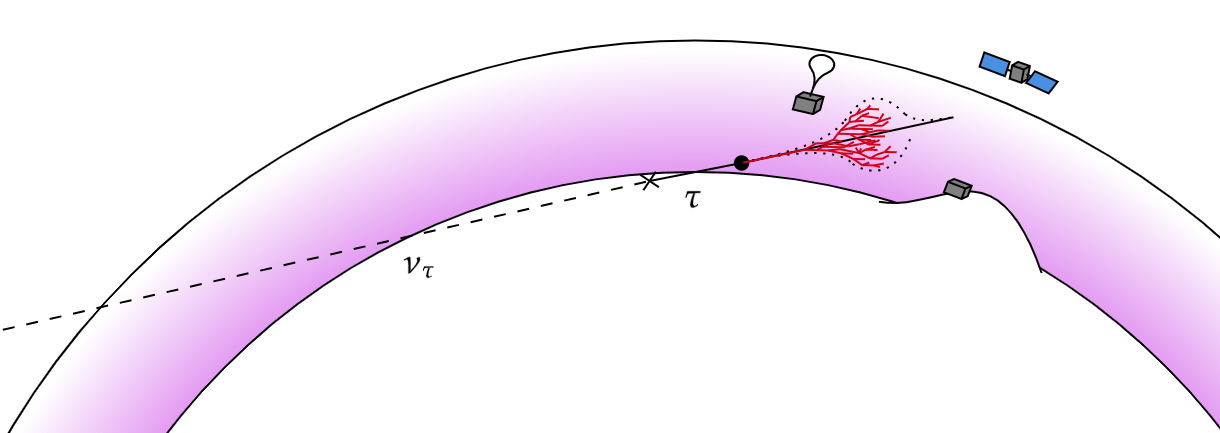
\includegraphics[width=.7\linewidth]{figures/shower_up}
		\caption{Propuesta de detección de neutrinos tau de origen astrofísico.}
		\label{shower_up}
	\end{figure}
La razón para considerar únicamente neutrinos tau\footnote{ Aunque en \eqref{ec11} vemos que las interacciones de UHECR en las fuentes darían una proporción $\nu_e:\nu_\mu:\nu_\tau\sim1:2:0$, las oscilaciones de sabor a lo largo de la propagación hacen que, a grandes distancias, $\nu_e:\nu_\mu:\nu_\tau\sim1:1:1$} reside simplemente en el hecho de que el leptón $\tau$ combina una poca probabilidad de interacción y pérdida de energía en el interior de la Tierra (los $e^\pm$ asociados a $\nu_e$ no llegarían a la atmósfera) con una vida media muy corta ($\sim 3\times10^{-13}\,\mathrm{s}$) que permite su desintegración dentro de la atmósfera y la aparición de una cascada (los $\mu^\pm$ asociados a $\nu_\mu$ \textit{escaparían} de la atmósfera sin generar una cascada, al tener vidas medias largas y pocas interacciones). 

Actualmente, existen numerosos experimentos entre cuyos objetivos se sitúan la detección de esta clase de eventos. Entre ellos podemos mencionar BEACON\footnote{ Beamforming Elevated Array for COsmic Neutrinos}, que aspira a medir el flujo de $\nu_\tau$ con $E>100\,\mathrm{PeV}$ mediante técnicas interferométricas a partir de datos recolectados en arrays de antenas dispuestas sobre montañas, o ANITA y su futuro sucesor PUEO\footnote{ANtarctic Impulsive Transient Antenna, Payload for Ultrahigh Energy Observations}, que permiten observar mediante antenas dispuestas en globos a gran altura ($\sim 36\,\mathrm{km}$) la radiación asociada a cascadas iniciadas en interacciones con el hielo de la Antártida.

Este trabajo se enmarca dentro de estas propuestas experimentales, y los desarrollos que haremos a continuación tendrán como objetivo describir y caracterizar tanto cascadas atmosféricas hacia arriba como la emisión en radiofrecuencias asociada, para comprobar la posibilidad de extraer información sobre la partícula primaria mediante observaciones a gran altitud.


	\clearpage
	\section{Cascadas atmosféricas}\label{sec2}
%	Fisica, conceptos, etc
%	
%	Comentar AIRES
%	
%	Meter simulaciones de desarrollo UG, CompUGDG

Las cascadas atmosféricas representan la opción más importante para lograr estudiar la radiación cósmica mas energética. Debido a los escasos flujos ($<1\,\mathrm{m^{-2}y^{-1}}$ a partir de $E=10^{15}\,\mathrm{eV}$), la detección directa de estas partículas, por ejemplo en detectores situados fuera de la atmósfera, se hace inviable. Por ello, el estudio de la radiación cósmica en esta región de energías se realiza observando las consecuencias de las interacciones de estas partículas en la atmósfera. 


\subsection{Desarrollo de cascadas en la atmósfera}\label{sec21}

Cuando un rayo cósmico de muy alta energía (por ejemplo un protón) llega a las capas superiores de la atmósfera e interacciona con la materia presente en el medio, producirá un número elevado de partículas secundarias, a su vez de altas energías, que volverán a generar más partículas sucesivamente. De este modo, se desarrolla una \textit{cascada} de partículas propagándose a través de la atmósfera, en la que el número de partículas continúa aumentando progresivamente, hasta que la energía de las partículas no es suficiente para mantener el crecimiento (i.e., se alcanza un máximo del desarrollo). Gracias al elevado número de partículas producidas en esta clase de eventos (hasta $10^{11}$ para las partículas primarias más energéticas), su estudio es posible mediante diversas técnicas (detectores de partículas a nivel de suelo, estudio de la fluorescencia provocada por las partículas en la atmósfera, medidas de la radiación \v{C}erenkov, ...). En cierto modo, la atmósfera actúa como un calorímetro que permite extraer información acerca de la energía y dirección de llegada del rayo cósmico primario, a partir de la deposición de energía en el medio en forma de una cascada atmosférica.

No obstante, usar la atmósfera como medio de detección tiene, evidentemente, la desventaja de que se trata de un medio inhomogéneo, en el que la densidad decrece con la altitud, $\rho = \rho(h)$. Como ejemplo, uno de los modelos más simples para la dependencia de la densidad con la altura es un decrecimiento exponencial:
\begin{equation}
	\rho(h)=\rho_0\exp\left(-h/h_0\right)\; \;;\;\;\text{donde}\;\rho_0\sim1,23\times 10^{-3}\,\mathrm{g/cm^3}\;\text{y}\;h_0\sim8,5\,\mathrm{km}\label{ec21}
\end{equation}

Naturalmente, este hecho tendrá consecuencias importantes en el desarrollo de la cascada. Fundamentalmente, el efecto se deberá a que, a mayor densidad, mayor probabilidad de interacción para las partículas producidas. Para tener en cuenta esta cuestión, gran parte de la discusión que haremos acerca del desarrollo de cascadas atmosféricas no se hará en términos de distancias, sino de cantidad de materia atravesada o \textit{profundidad}, $X$. Dicha profundidad puede medirse en la dirección vertical ($X_v$) o a lo largo del eje ($X_s$) del desarrollo de la cascada (Fig. \ref{shower_params}):
\begin{equation}
	X_v(h)=\int_{h}^\infty\rho(h')dh'\;\;;\;\;X_s(h,\theta)=\int_{h}^\infty\rho(h')dl=\int_h^{\infty}\rho(h')\frac{dh'}{\sqrt{1-\frac{R_T^2\sin^2{\theta}}{\left(R_T+h'\right)^2}}}\label{ec22}
\end{equation}
Gracias a estas definiciones, podremos estudiar el desarrollo de cascadas en términos de magnitudes que inmediatamente incorporan la inhomogeneidad de la atmósfera, por lo que no profundizaremos más en los modelos que describen la atmósfera y pasaremos a cuestiones de mayor interés para el objetivo de este trabajo.

\begin{figure}[H]
	\centering
	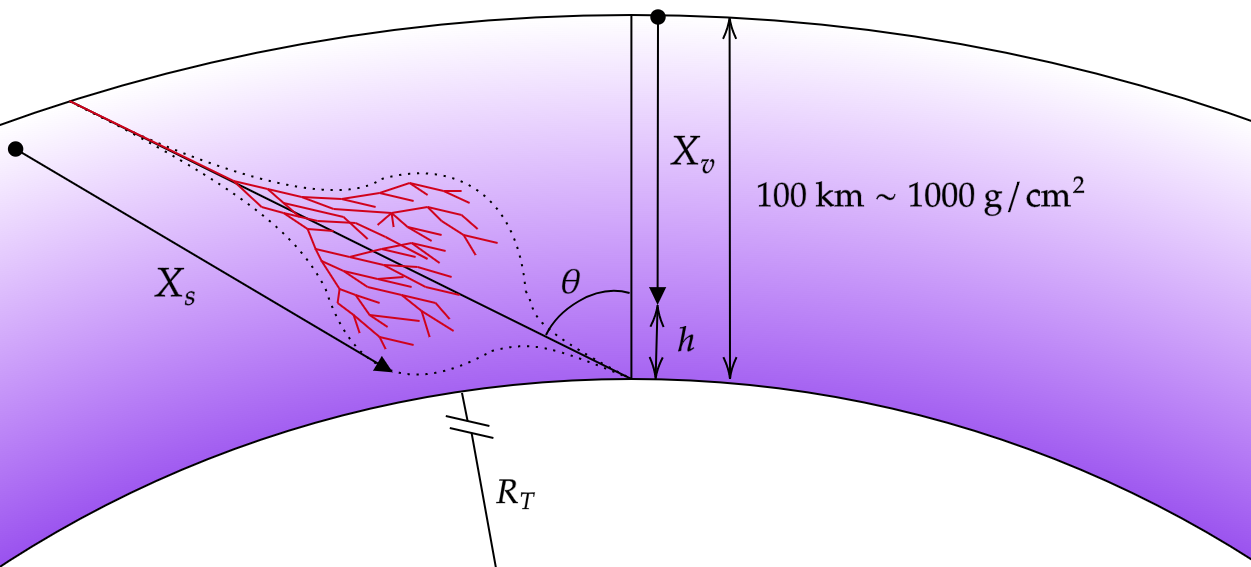
\includegraphics[width=.7\linewidth]{figures/cascadas/shower_params}
	\caption{Esquema simplificado de una cascada atmosférica \textit{al uso}. Definición de profundidad vertical e inclinada (\textit{slanted}). $R_T$ es el radio de la Tierra.}
	\label{shower_params}
\end{figure}

Como hemos mencionado en el apartado introductorio, nos interesará estudiar cascadas atmosféricas que se propagan \textit{hacia arriba}, y además iniciadas por la desintegración de un leptón $\tau$. En esta clase de situación, por tanto, tendremos una cascada propagándose desde zonas más a menos densas, y que pueden haber sido iniciadas por leptones o hadrones de alta energía (ya que los abundantes modos de desintegración del $\tau$ permiten la producción de ambos tipos de partículas). Por ello, para poder comprender estos eventos, comenzaremos por repasar brevemente las tres \textit{componentes} diferenciadas que pueden aparecer en una cascada atmosférica y su evolución a lo largo del desarrollo de la misma.
\begin{itemize}
	\item\textit{Componente electromagnética}: Integrada, fundamentalmente, por fotones, electrones y positrones; que representan las partículas más abundantes en una cascada atmosférica. A altas energías\footnote{ Mayores a la energía crítica $E_C\sim86\,\mathrm{MeV}$, en la que las pérdidas de energía por ionización superan a las de bremsstrahlung.}, las interacciones que multiplican el número de partículas asociadas a esta componente serán la producción de pares ($\gamma+\text{Nuc.}\rightarrow e^+e^-+\text{Nuc.}$) y bremsstrahlung ($e^\pm+\text{Nuc.}\rightarrow e^\pm+\gamma+\text{Nuc.}$). Cuando la energía de las partículas baja lo suficiente, aparecen pérdidas de energía mediante interacciones con los electrones del medio (scattering Compton, ionizaciones y excitaciones, aniquilación $e^+e^-$, ...) que detienen el desarrollo de la cascada.
	\item\textit{Componente hadrónica}: Integrada por protones, núcleos, piones y demás hadrones. En este caso, las interacciones más relevantes serán las de producción de piones ($p+\text{Nuc.}\rightarrow\pi^0,\pi^\pm,p,...$ ; $\pi^0+\text{Nuc.}\rightarrow \pi^0,\pi^\pm,...$). Además, a altas energías, el número de partículas producidas en cada interacción será muy superior al de los procesos electromagnéticos ($\gtrsim75$ secundarios en cada interacción). A diferencia de la componente electromagnética, en este caso debemos considerar también procesos de desintegración que alimentarán otras componentes:
	\begin{itemize}
		\item $\pi^0\rightarrow\gamma\gamma$ ($\tau\sim8,4\times10^{-17}\,\mathrm{s}$). Alimenta la componente electromagnética.
		\item  $\pi^+\rightarrow\mu^+\nu_\mu$ ; $\pi^-\rightarrow\mu^-\bar\nu_\mu$ ($\tau\sim2,6\times10^{-8}\,\mathrm{s}$). Alimenta la componente muónica.
	\end{itemize}
Dada la pequeña vida media del $\pi^0$, podemos asumir con seguridad que la gran mayoría de piones neutros producidos se desintegran antes de interaccionar. Dado que la producción de cada tipo de pión es equiprobable, en cada interacción podemos tomar la aproximación de que $1/3$ de la energía se \textit{transfiere} a la componente electromagnética, cuyo origen en cascadas iniciadas por hadrones estará precisamente en este proceso. Eventualmente, la mayoría de la energía asociada a hadrones se habrá transferido a la componente EM, y se acabará disipando en ionizaciones y excitaciones del medio.

Por otra parte, la desintegración del pión cargado alimenta la componente muónica, cuyas interacciones con el medio serán prácticamente despreciables, sufriendo muy poca atenuación en la atmósfera. No obstante, la vida media más larga del $\pi^\pm$ hace que las interacciones que multiplican el número de piones sean relevantes hasta que las energías bajan de $\sim 20\,\mathrm{GeV}$.
	\item\textit{Componente muónica}: Integrada por muones y neutrinos producidos, fundamentalmente, en la desintegración del pión cargado. La interacción de estas partículas en la atmósfera será prácticamente despreciable. Por otra parte, la larga vida media del muón ($\mu\rightarrow e\nu_e\nu_\mu$, $\tau\sim2\times10^{-6}\,\mathrm{s}$) hace que en la mayoría de los casos atraviesen la atmósfera sin desintegrarse.
\end{itemize}

En general, el desarrollo de las cascadas atmosféricas está determinado por la competición entre interacción y desintegración que afecta a los hadrones. Si las interacciones dominan, el número de partículas se multiplica y la cascada \textit{crece}, mientras que las desintegraciones alimentan la componente EM y muónica, que \textit{extraen} energía de la cascada y detienen su desarrollo. Mientras que las desintegraciones sólo dependen de la energía de la partícula y el tiempo de propagación, las interacciones dependen de la cantidad de materia atravesada, que como hemos visto depende de la altura en la atmósfera. Dos magnitudes clave en este aspecto que podrán ser útiles más adelante son la \textit{distancia de interacción y desintegración}:
\begin{itemize}
	\item \textit{Distancia de interacción,} $\lambda_I\,\left[\mathrm{g/cm^2}\right]$: Cantidad de materia que debe atravesarse para que, en promedio, ocurra una interacción. En uds. de distancia, $d_I\sim\lambda_I/\rho(h)$. Para el caso de los piones interaccionando con aire:
\begin{equation}
		\lambda_I=70-120\,\mathrm{g/cm^2}\label{ec23}
\end{equation}

\item \textit{Distancia de desintegración, }$d_{dec}\,\left[\mathrm{m}\right]$: Distancia promedio que recorre una partícula antes de decaer. Depende de la vida media en reposo y la energía. En el caso de los piones:
\begin{equation}
	d_{dec}=\gamma\beta c\tau\sim\frac{E}{mc^2}c\tau\left\{\begin{array}{l}\pi^\pm\rightarrow d_{dec}=\gamma\left(7,8 \,\mathrm{m}\right)\\
\pi^0\rightarrow d_{dec}=\gamma\left(2,5\times10^{-8}\,\mathrm{m}\right)\end{array}\right.
\label{ec24}
\end{equation}
\end{itemize}
Naturalmente, la energía a la que $d_{dec}\sim\lambda_I/\rho$ determina el punto en que las interacciones comienzan a verse superadas por las desintegraciones:
\begin{equation}
	d_{dec}\sim\lambda_I/\rho\implies E_{dec}\sim \frac{\lambda_I mc^2}{\rho c \tau}\label{edec}
\end{equation} Por lo tanto, estas magnitudes nos permiten estimar, de manera sencilla, en qué fase del desarrollo se encuentra cada componente de la cascada. Además, vemos claramente las dependencias tanto con la densidad como con la energía en \eqref{ec23} y \eqref{ec24}. Por lo tanto, podemos intuir que habrá diferencias sustanciales entre una cascada \textit{habitual} en que las partículas de mayor energía aparecen en las zonas menos densas de la atmósfera, y una cascada hacia arriba en que las partículas más energéticas aparecen en la región de mayor densidad para propagarse hacia zonas menos densas. Exploraremos esta posibilidad a continuación.

	\subsection{Caracterización de cascadas atmosféricas hacia arriba}\label{sec22}
	Para poder comprender mejor la evolución de cascadas atmosféricas en general, y más concretamente el caso de las cascadas propagándose \textit{hacia arriba}, hemos realizado una serie de simulaciones recurriendo al código AIRES \cite{https://doi.org/10.13140/rg.2.2.12566.40002} que nos permitirán explorar las características del desarrollo de las partículas más abundantes en cascadas atmosféricas (fundamentalmente nos centraremos en $e^\pm$, $\mu^\pm$ y $\pi^\pm$) en función de la naturaleza y energía del primario, de la altura a la que ocurre la primera interacción o el ángulo con el que se desarrolla la cascada. Naturalmente, el crecimiento del número de partículas cargadas en la atmósfera marcará la emisión de radiación en cascadas atmosféricas, así que nos detendremos en estudiar este aspecto en esta sección antes de avanzar en el objetivo de este trabajo.
	
	AIRES es un código capaz de simular mediante técnicas Monte Carlo el desarrollo de cascadas atmosféricas a nivel microscópico, i.e., teniendo en cuenta las interacciones que tienen lugar a lo largo de la evolución de la cascada y la propagación en el medio. Debido al elevado número de partículas que se producen, es necesario recurrir a un algoritmo de \textit{muestreo} que estudia la propagación de partículas \textit{estadísticamente relevantes}, para luego compensar adecuadamente la contribución de las partículas rechazadas. Gracias a este procedimiento, es posible estudiar el desarrollo de la cascada en un número de horas de CPU \textit{asumibles}. Además, el propio código incorpora modelos detallados de la atmósfera y campo magnético terrestre, lo que permite añadir condiciones plenamente realistas para el desarrollo de las cascadas.
	
	Para poner de manifiesto el detalle con que AIRES permite simular el desarrollo de cascadas, en la siguiente Tabla se recogen las partículas e interacciones consideradas en las simulaciones:
\begin{table}[H]
	\centering
	\begin{tabular}{clc}
		\hline
		\multicolumn{2}{c}{Partícula}                                                                   & Interacciones                         \\ \hline
		\multicolumn{2}{c}{\multirow{5}{*}{\begin{tabular}[c]{@{}c@{}}$\gamma$\\ $e^\pm$\end{tabular}}} & Efectos Compton y fotoeléctrico       \\
		\multicolumn{2}{c}{}                                                                            & Bremsstrahlung y producción de pares  \\
		\multicolumn{2}{c}{}                                                                            & Aniquilación $e^+e^-$                 \\
		\multicolumn{2}{c}{}                                                                            & Emisión de $e^-$ knock-on             \\
		\multicolumn{2}{c}{}                                                                            & Reacciones fotonucleares, ...         \\ \hline
		\multicolumn{2}{c}{\multirow{3}{*}{$\mu^\pm$}}                                                  & Bremsstrahlung y producción de pares  \\
		\multicolumn{2}{c}{}                                                                            & Emisión de $e^-$ knock-on             \\
		\multicolumn{2}{c}{}                                                                            & Desintegración                        \\ \hline
		\multicolumn{2}{c}{$\nu$'s}                                                                   & Aparición en desintegraciones         \\ \hline
		\multicolumn{2}{c}{$p,\bar p, n, \bar n, \Lambda$}                                              & Colisiones hadrónicas y núcleo-núcleo \\
		\multicolumn{2}{c}{$\pi^0, \pi^\pm, K^0_{L,S}, K^\pm$}                                          & Emisión de $e^-$ knock-on             \\
		\multicolumn{2}{c}{Núcleos $Z\leq 36$}                                                          & Desintegraciones                      \\ \hline
	\end{tabular}
\caption{Partículas e interacciones consideradas en AIRES (v. 2.6)}
\end{table}

El estudio de la evolución de la cascada en AIRES se puede realizar, entre otras maneras, estableciendo una serie de \textit{niveles de observación} a lo largo del desarrollo. En cada uno de ellos, se registran las partículas que lo atraviesan y su energía, permitiendo obtener el desarrollo longitudinal del número de partículas y su energía. Los niveles de observación se disponen equiespaciados en profundidad atravesada, bien a lo largo del eje de desarrollo de la cascada ($X_s$) o en la dirección vertical ($X_v$):
\clearpage
	\begin{figure}[H]
		\centering
		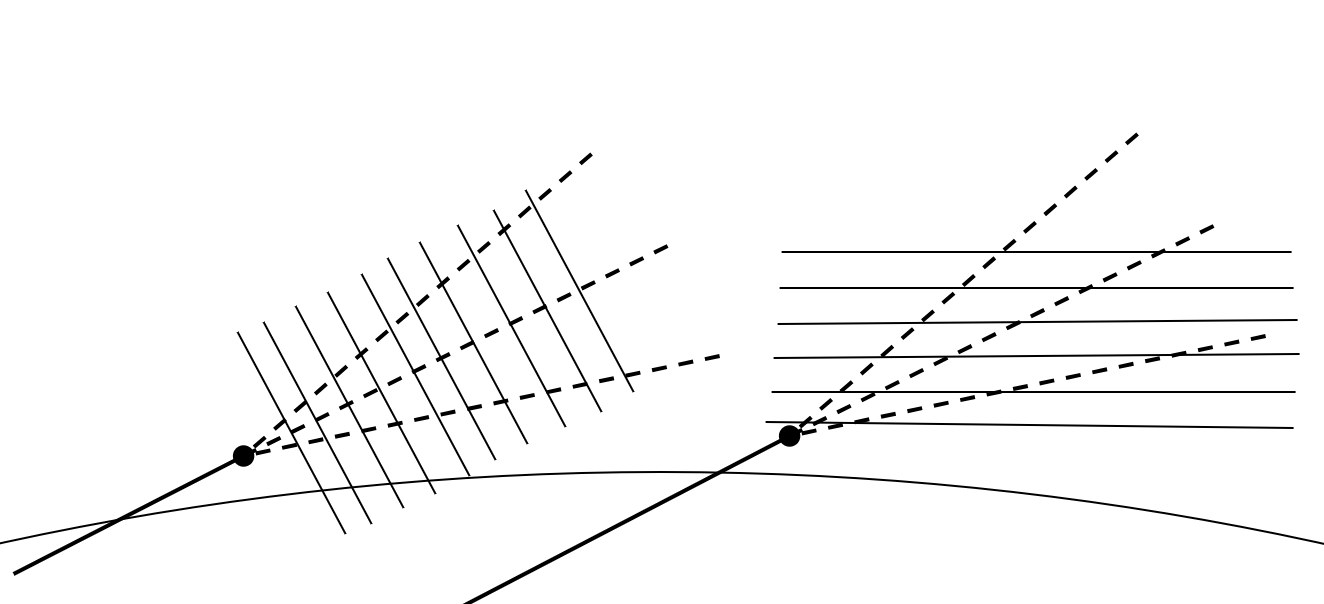
\includegraphics[width=.6\linewidth]{figures/cascadas/AIRES_planos}
		\caption{Disposiciones posibles de los niveles de observación en AIRES, en el ejemplo de una cascada hacia arriba. Izq.: A lo largo del eje del desarrollo. Der.: Dirección vertical.}
		\label{AIRES_planos}
	\end{figure}
	
%Aunque presentaremos algún resultado con la configuración de la derecha en la Fig. anterior, normalmente optaremos por situar los niveles de observación a lo largo del eje del desarrollo\footnote{ Aunque a priori parezca irrelevante, la elección de niveles de observación tiene efectos no triviales en los valores obtenidos de la simulación, como comprobaremos en algún caso.}. 
Además, dado que conocemos el modelo atmosférico\footnote{ AIRES emplea la parametrización de Linsley.}, podremos convertir la posición de los planos de observación a alturas o distancias \textit{recorridas} en la atmósfera aplicando \eqref{ec22}, lo que nos permitirá estudiar el desarrollo de las cascadas en varios términos. Teniendo en mente el funcionamiento de las simulaciones, podemos pasar a discutir el desarrollo de cascadas hacia arriba en la atmósfera.

Fundamentalmente, existen cuatro aspectos básicos que afectarán al desarrollo de estas cascadas: el ángulo de inclinación, la altura en la atmósfera a la que ocurre la primera interacción, y la naturaleza y energía de la partícula primaria que inicia la cascada. Para estudiar los efectos de cada una de estas cuestiones, presentaremos y discutiremos a continuación una serie de resultados de simulaciones con AIRES variando cada una de las magnitudes que acabamos de mencionar.
\begin{itemize}
	\item \textit{Ángulo de la cascada}:
\end{itemize}
	La dependencia del desarrollo con el ángulo de inclinación del eje de la cascada es evidente si recordamos la dependencia de la densidad con la altura en la atmósfera. Para ilustrar esta idea, hemos representado en la Fig. \ref{Profatravesadavsang} la cantidad de materia atravesada desde el nivel del suelo hacia arriba para varios ángulos, usando una expresión equivalente\footnote{ Simplemente integrando entre $0$ y $h$.} a \eqref{ec22}. Como vemos, la cantidad de materia atravesada en la atmósfera aumenta cuanto más \textit{horizontal} sea la cascada por lo que esperaremos, por ejemplo, la producción de un mayor número de partículas en ese caso, al dominar las interacciones en regiones más densas.
	
	Antes de presentar resultados, debemos comentar el criterio empleado para los ángulos de inclinación de la cascada: para cascadas \textit{hacia abajo}, indicaremos el ángulo en el intervalo $\theta\in[0^\circ, 90^\circ]$ (Fig. \ref{shower_params}), mientras que en cascadas hacia arriba, por consistencia, daremos el ángulo en el intervalo  $\theta\in[90^\circ, 180^\circ]$, siendo $
	90^\circ$ ($180^\circ$) una cascada horizontal (vertical hacia arriba).
\clearpage
	\begin{figure}[H]
		\centering
		\includegraphics[width=.7\linewidth]{figures/cascadas/Profatravesadavsang}
		\caption{Cantidad de materia atravesada a lo largo del eje de la cascada (hacia arriba) en función de la altura en la atmósfera, para varios ángulos. El gradiente de color que representa la atmósfera sigue la dependencia \eqref{ec21}, empleada para realizar esta gráfica. Se ha tenido en cuenta la curvatura de la Tierra,  la primera imagen es meramente ilustrativa.}
		\label{Profatravesadavsang}
	\end{figure}

Con esto en mente, presentamos en la Fig. \ref{Carac_UG_vardeg} los resultados de la simulación en AIRES del desarrollo longitudinal de electrones, positrones, muones y piones cargados para cascadas hacia arriba iniciadas por un protón de energía $1\,\mathrm{EeV}$ interaccionando a $5\,\mathrm{km}$ de altura en la atmósfera, para varios ángulos de inclinación.

La primera observación que podemos hacer es que, como acabamos de mencionar, el máximo número de partículas producido en la cascada decrece al aumentar el ángulo, i.e., cuanto más \textit{vertical} se sitúa el eje de la cascada. Por otra parte, vemos en las gráficas correspondientes del desarrollo frente a la profundidad atravesada \textit{a lo largo} del eje de la cascada que el máximo de la cascada ocurre aproximadamente en la misma posición, un resultado natural ya que esperamos que la producción de partículas dependa de la materia atravesada. Al tener en cuenta la inclinación, es evidente que las cascadas más verticales deberán recorrer más distancia para atravesar la misma cantidad de materia, por lo que los máximos aparecen desplazados en $X_v$ (véanse Figs. \ref{AIRES_planos} y \ref{Profatravesadavsang}). 

No obstante, en las gráficas frente a $X_s$ observamos, para el caso de $\mu^\pm$ y $\pi^\pm$, que la posición del máximo cambia ligeramente con el ángulo, algo que no ocurre en el caso de los electrones. La diferencia entre ambos casos es la existencia de desintegraciones. Para interpretar este hecho, podemos ver en \eqref{edec} que la energía a la que las desintegraciones comienzan a dominar aumentará con la inclinación (dependencia $\rho^{-1}$, la zona densa se abandona antes), por lo que se alcanzará el máximo en un menor número de interacciones. Vemos por otra parte que el comportamiento de los desarrollos de piones cargados y muones es muy similar, con cierto \textit{retardo} que nos indica que el origen de los muones está en la desintegración del $\pi^\pm$. Además, apreciamos en la gráfica de desarrollo de muones frente a $X_v$, un ligero cambio de pendiente hacia el final del desarrollo, que evidencia sus desintegraciones.

Por último, en las gráficas del desarrollo frente a la distancia recorrida en la atmósfera, el ligero desplazamiento en las posiciones de los máximos de nuevo señala el hecho de que, cuanto mayor sea el ángulo, más altura debe alcanzarse en la atmósfera para atravesar la cantidad de materia necesaria para llegar al máximo. Además, en el caso de los $e^\pm$ vemos que la caída del número de partículas, que se debe a la pérdida de energía con el medio, es más rápida cuanto menor el ángulo, debido a que en ese caso aún habrá materia con la que interaccionar \textit{por delante}.

\begin{figure}[H]
	\centering
	\subfigure[$e^\pm$]{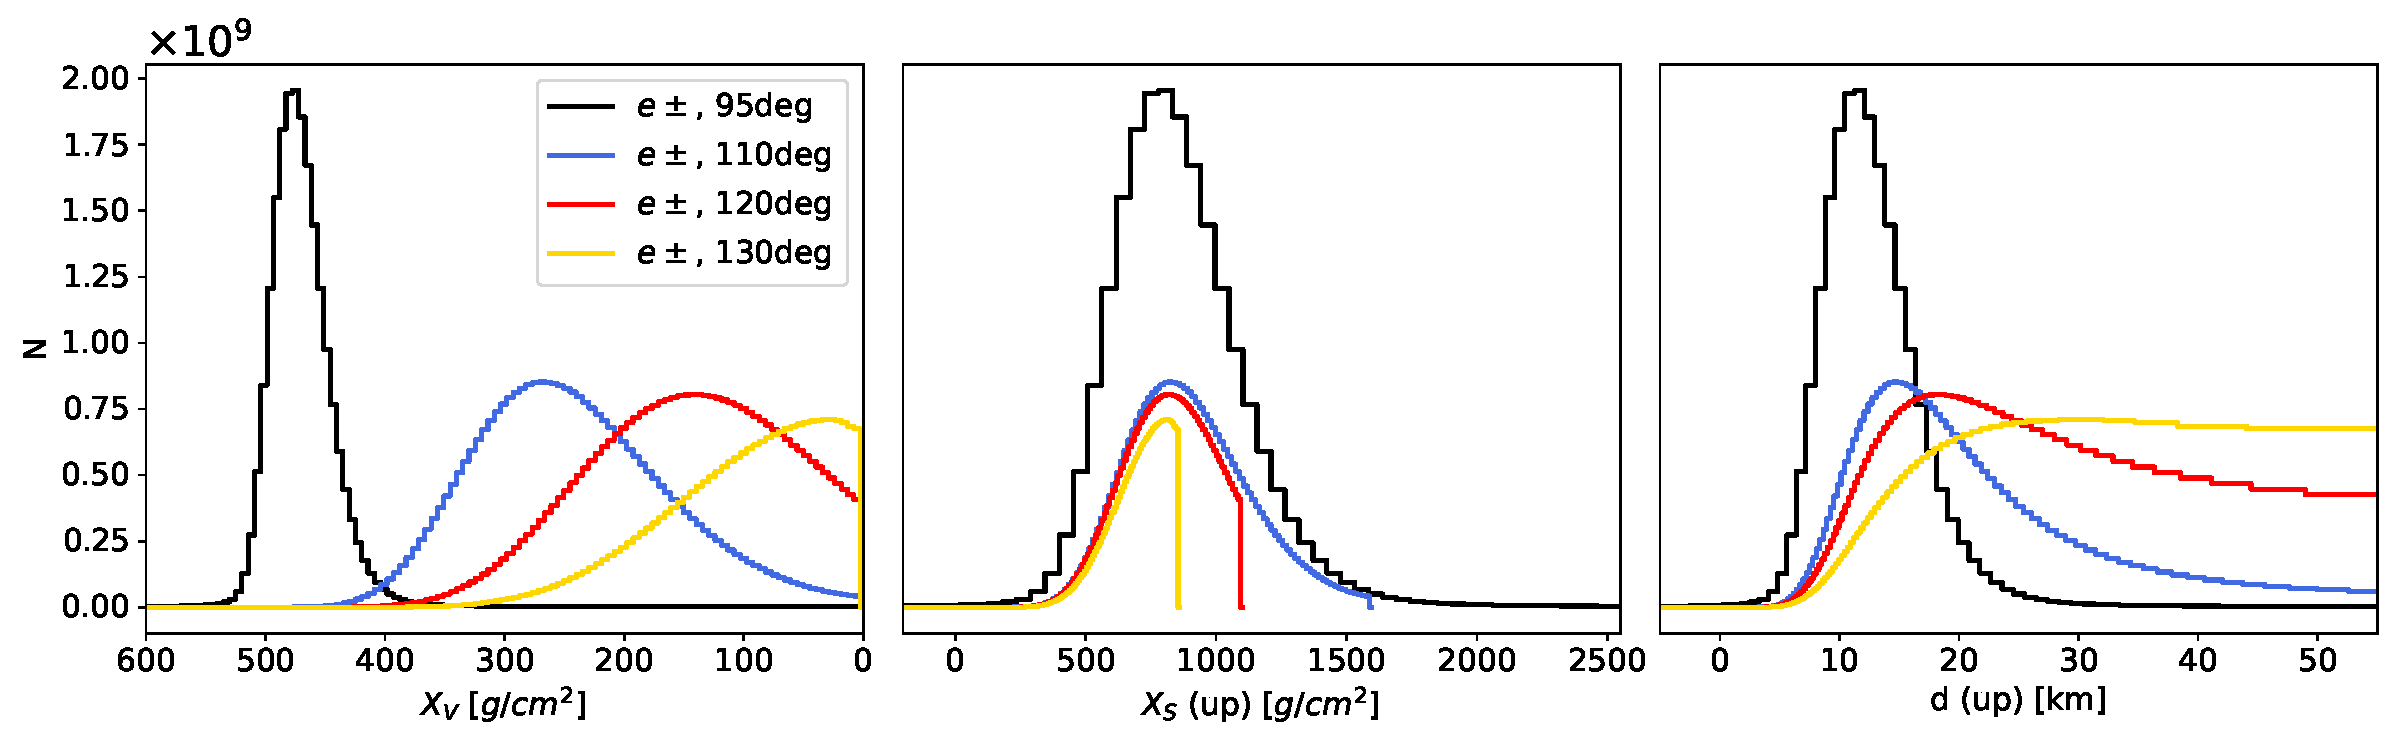
\includegraphics[width=1\linewidth]{figures/cascadas/upgoing_p_1EeV_vardeg_5km_e_v2}}
	\\
	\subfigure[$\mu^\pm$]{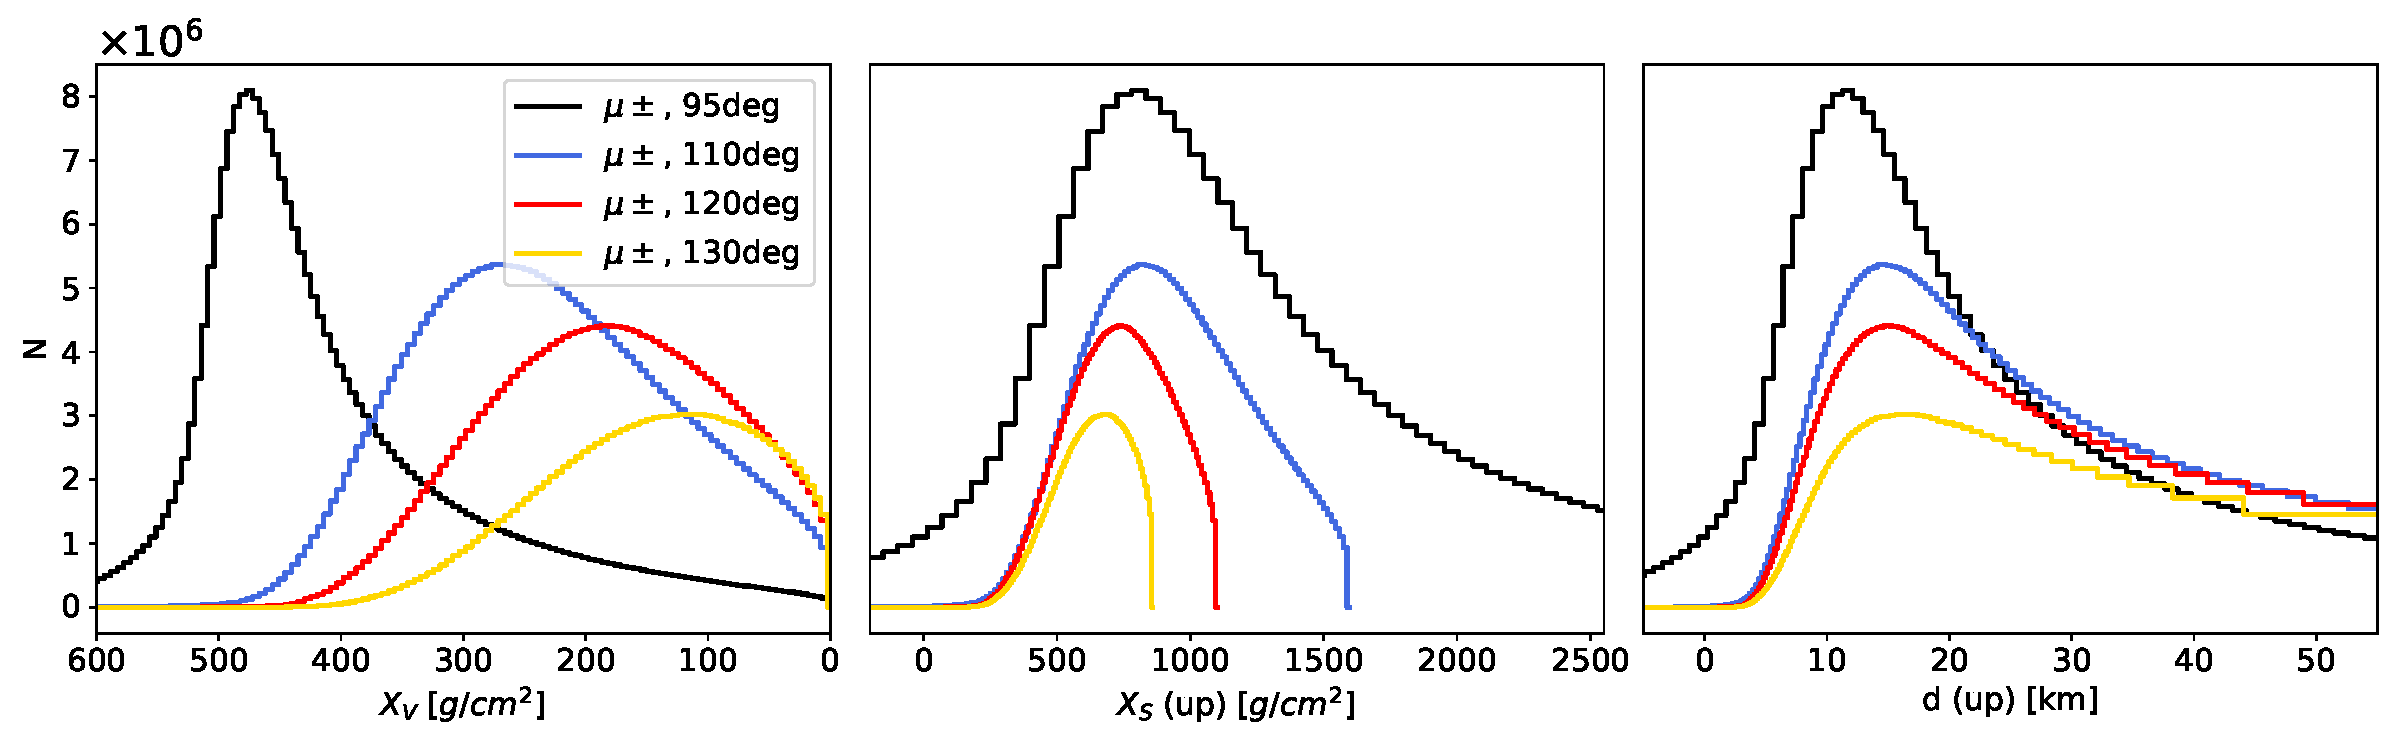
\includegraphics[width=1\linewidth]{figures/cascadas/upgoing_p_1EeV_vardeg_5km_mu_v2}}
	\\
	\subfigure[$\pi^\pm$]{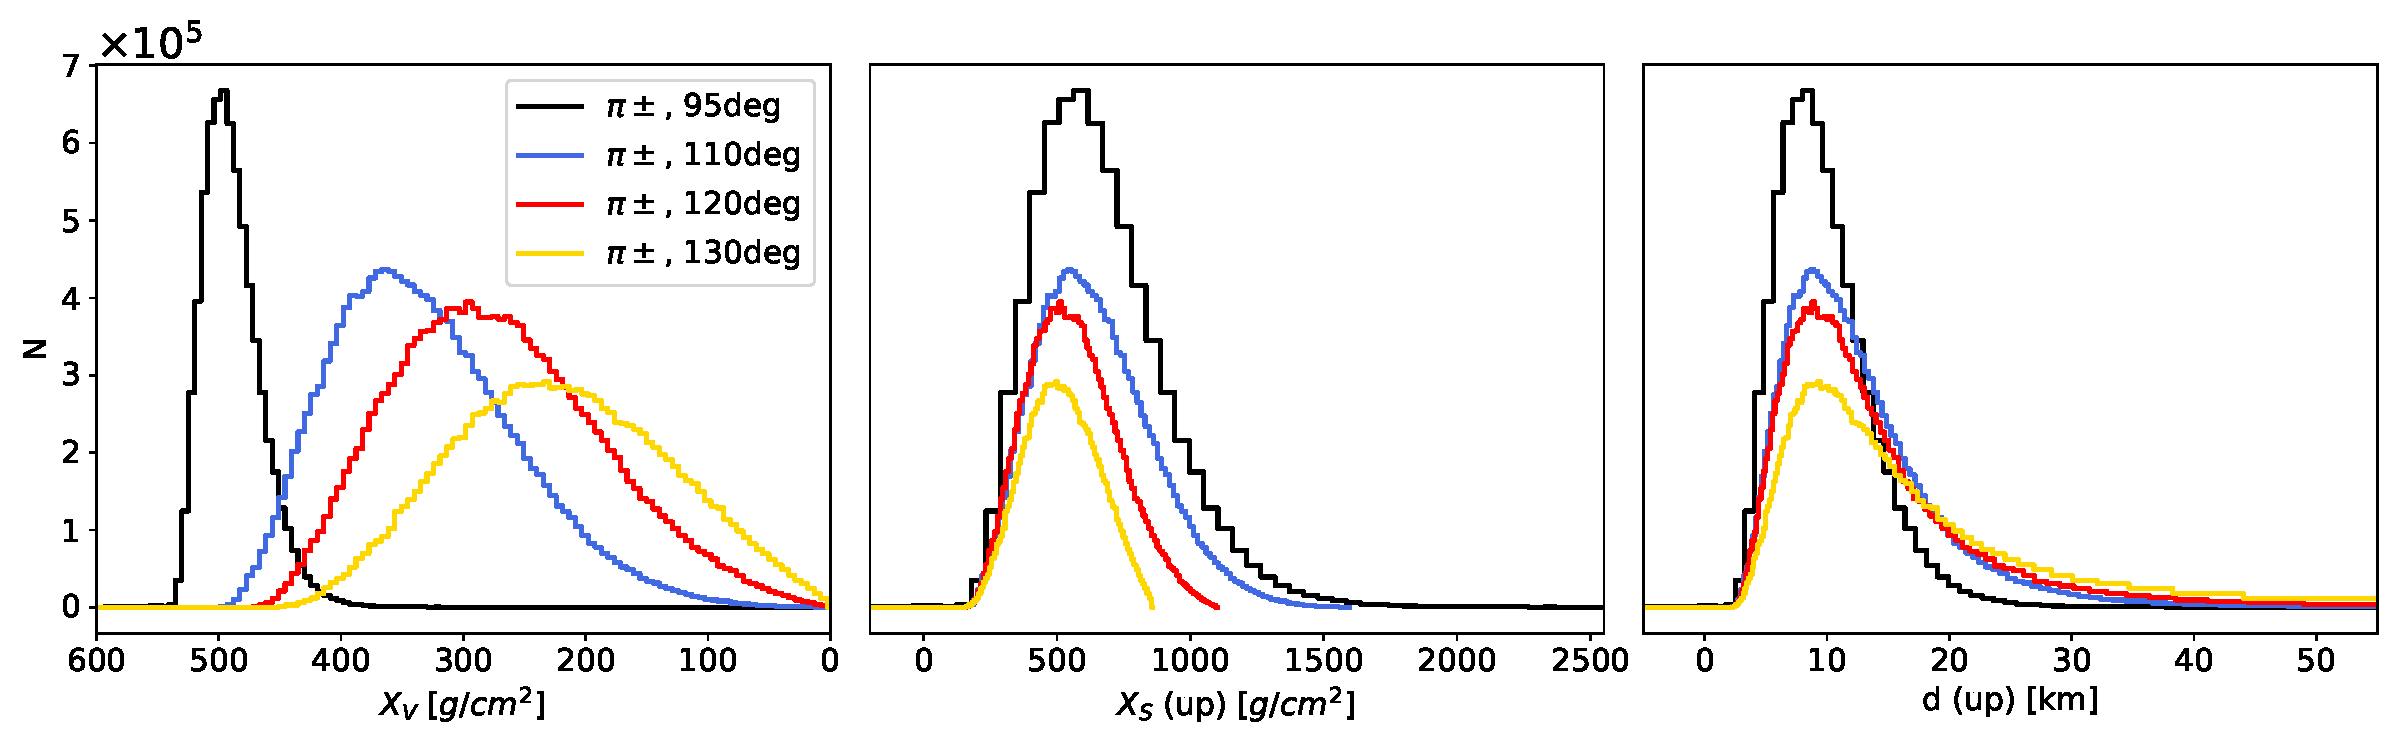
\includegraphics[width=1\linewidth]{figures/cascadas/upgoing_p_1EeV_vardeg_5km_pi_v2}}
	\caption{Desarrollo de electrones, muones y piones, en una cascada iniciada por un protón de $1\,\mathrm{EeV}$ interaccionando a $5\,\mathrm{km}$ de altura. Profundidad a lo largo del eje y distancia se miden desde el punto de primera interacción, i.e,  $h=5\,\mathrm{km}$. Los cortes en las gráficas vs. $X_s$ ($e^\pm$, $\mu^\pm$) marcan el final de la atmósfera.}
	\label{Carac_UG_vardeg}
\end{figure}
\begin{itemize}
	\item \textit{Altura de la primera interacción}
\end{itemize}
El punto de la atmósfera en que ocurra la primera interacción, y por lo tanto comience el desarrollo de la cascada, podrá afectar a dos cuestiones: el número de partículas producidas y la posición del máximo de la cascada. Para verlo, presentamos a continuación resultados de AIRES para el desarrollo de electrones, positrones y muones en una cascada de ángulo $\theta=95^\circ$ iniciada por un protón de energía $1\,\mathrm{EeV}$:
\begin{figure}[H]
	\centering
	\subfigure[$e^\pm$]{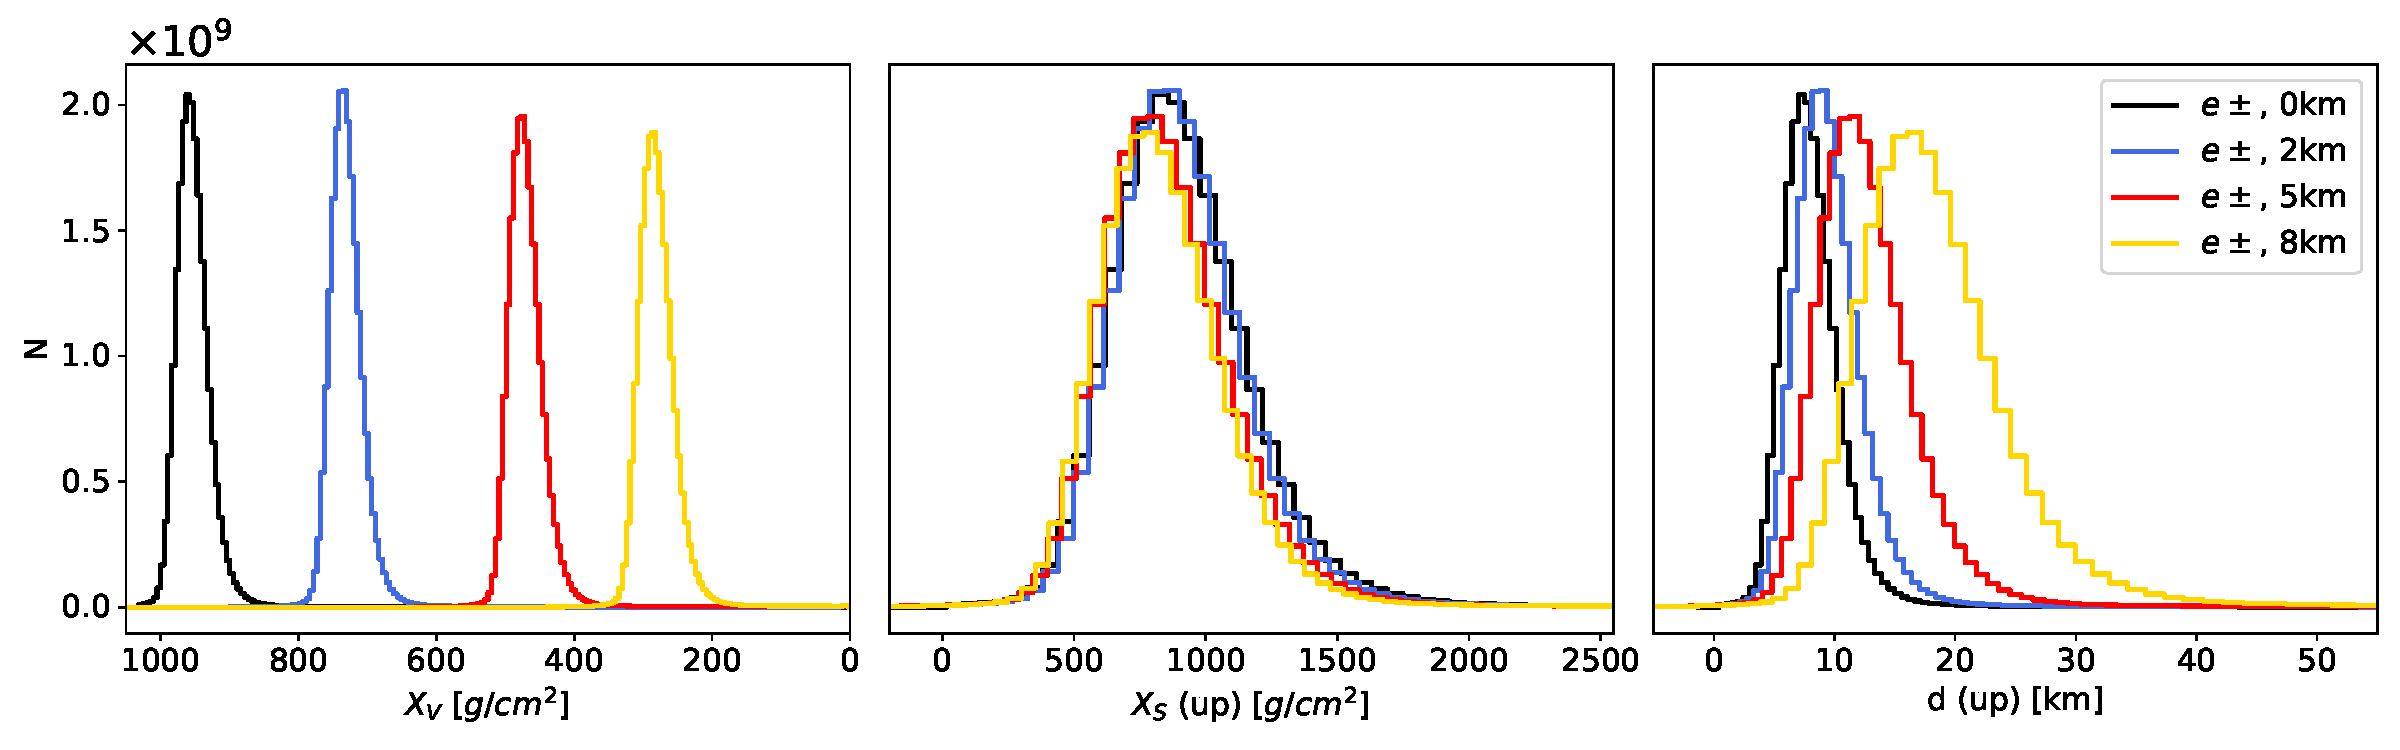
\includegraphics[width=1\linewidth]{figures/cascadas/upgoing_p_1EeV_95deg_varh_e_v2}}
	\\
	\subfigure[$\mu^\pm$]{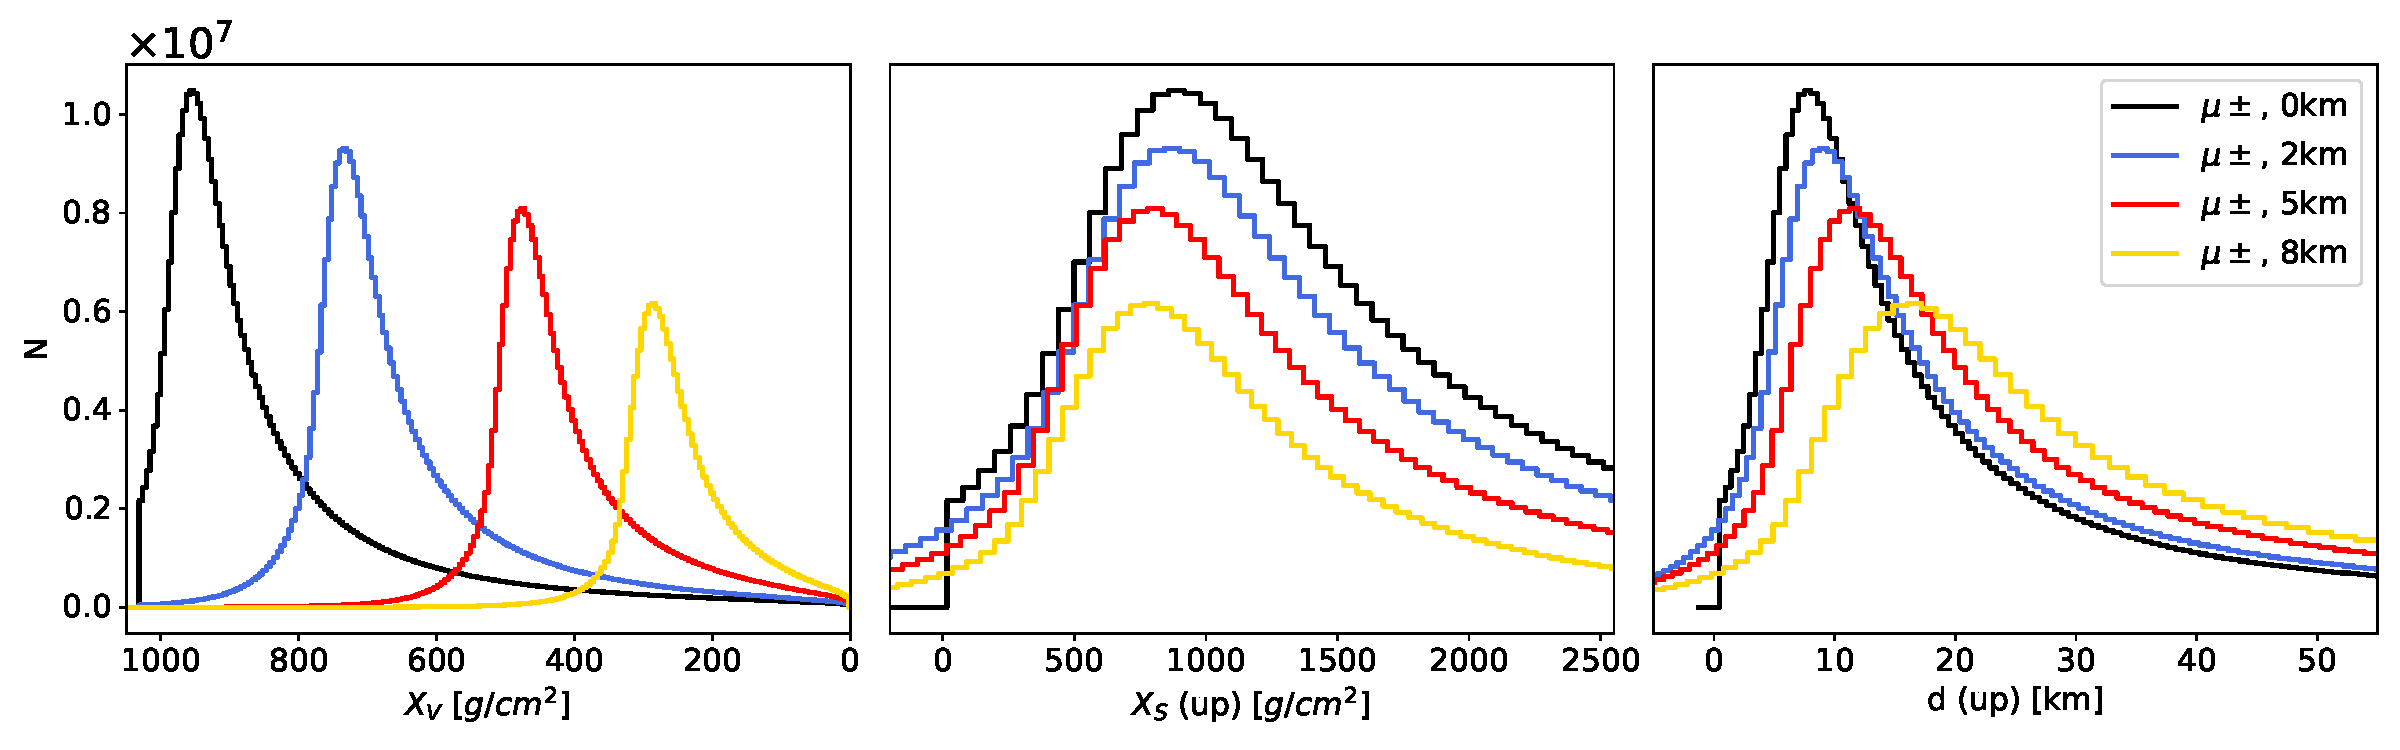
\includegraphics[width=1\linewidth]{figures/cascadas/upgoing_p_1EeV_95deg_varh_mu_v2}}

	\caption{Desarrollo de electrones y muones en una cascada a $95^\circ$ iniciada por un protón de $1\,\mathrm{EeV}$ interaccionando a varias alturas. $X_s$ y $d$ se miden desde la primera interacción.}
	\label{Carac_UG_varh}
\end{figure}
En primer lugar, la posición del máximo de la cascada cambia con la altura, un resultado evidente ya que estamos modificando el punto en que se inicia la cascada. Por su parte, en las gráficas frente a profundidad y distancia  a lo largo del eje volvemos a encontrar los mismos efectos que en el caso de la Fig. \ref{Carac_UG_vardeg}, sólo que ahora la diferencia en la materia atravesada viene dada por la altura de \textit{inyección} del primario y no por el ángulo de la cascada; pero la interpretación es la misma.

Quizá el efecto más interesante aparece en el número máximo de partículas. En el caso de los electrones apenas hay cambios con la altura, mientras que para los muones se aprecia un decrecimiento considerable al aumentar la misma. Como habíamos comentado, el desarrollo de las cascadas atmosféricas es tal que, eventualmente, la mayor parte de la energía acaba transfiriéndose a la componente electromagnética (a través de la desintegración de piones neutros, por ejemplo). Por ello, dado que la energía del primario es constante en estas simulaciones y las alturas consideradas son suficientemente bajas para que la cascada complete su desarrollo, el número de electrones es aproximadamente el mismo en todos los casos. No ocurre así con la producción de muones, que depende básicamente de las interacciones hadrónicas que dan lugar a piones cargados. Al aumentar la altura, debe recorrerse cada vez más distancia para atravesar la misma cantidad de materia ($\lambda_I$), reduciendo la tasa de interacciones y por tanto el número de muones que se produce. El mismo efecto se observa en la producción de piones, que no incluimos al verse representada en la evolución del número de muones.
\begin{itemize}
	\item \textit{Energía del primario}
\end{itemize}
Naturalmente, el desarrollo de la cascada estará muy afectado por la energía de la partícula primaria que la origina. Cunato mayor sea esta, mayor será el número de interacciones que ocurran así como el número de partículas producidas en cada interacción. Por ello, una de las consecuencias fundamentales de una mayor o menor energía del primario aparecerá en el número de partículas máximo. Como ejemplo, presentamos a continuación los resultados de la simulación de cascadas a $95^\circ$ iniciadas por un protón de energía variable, interaccionando a $5\,\mathrm{km}$ de altura: 
\begin{figure}[H]
	\centering
	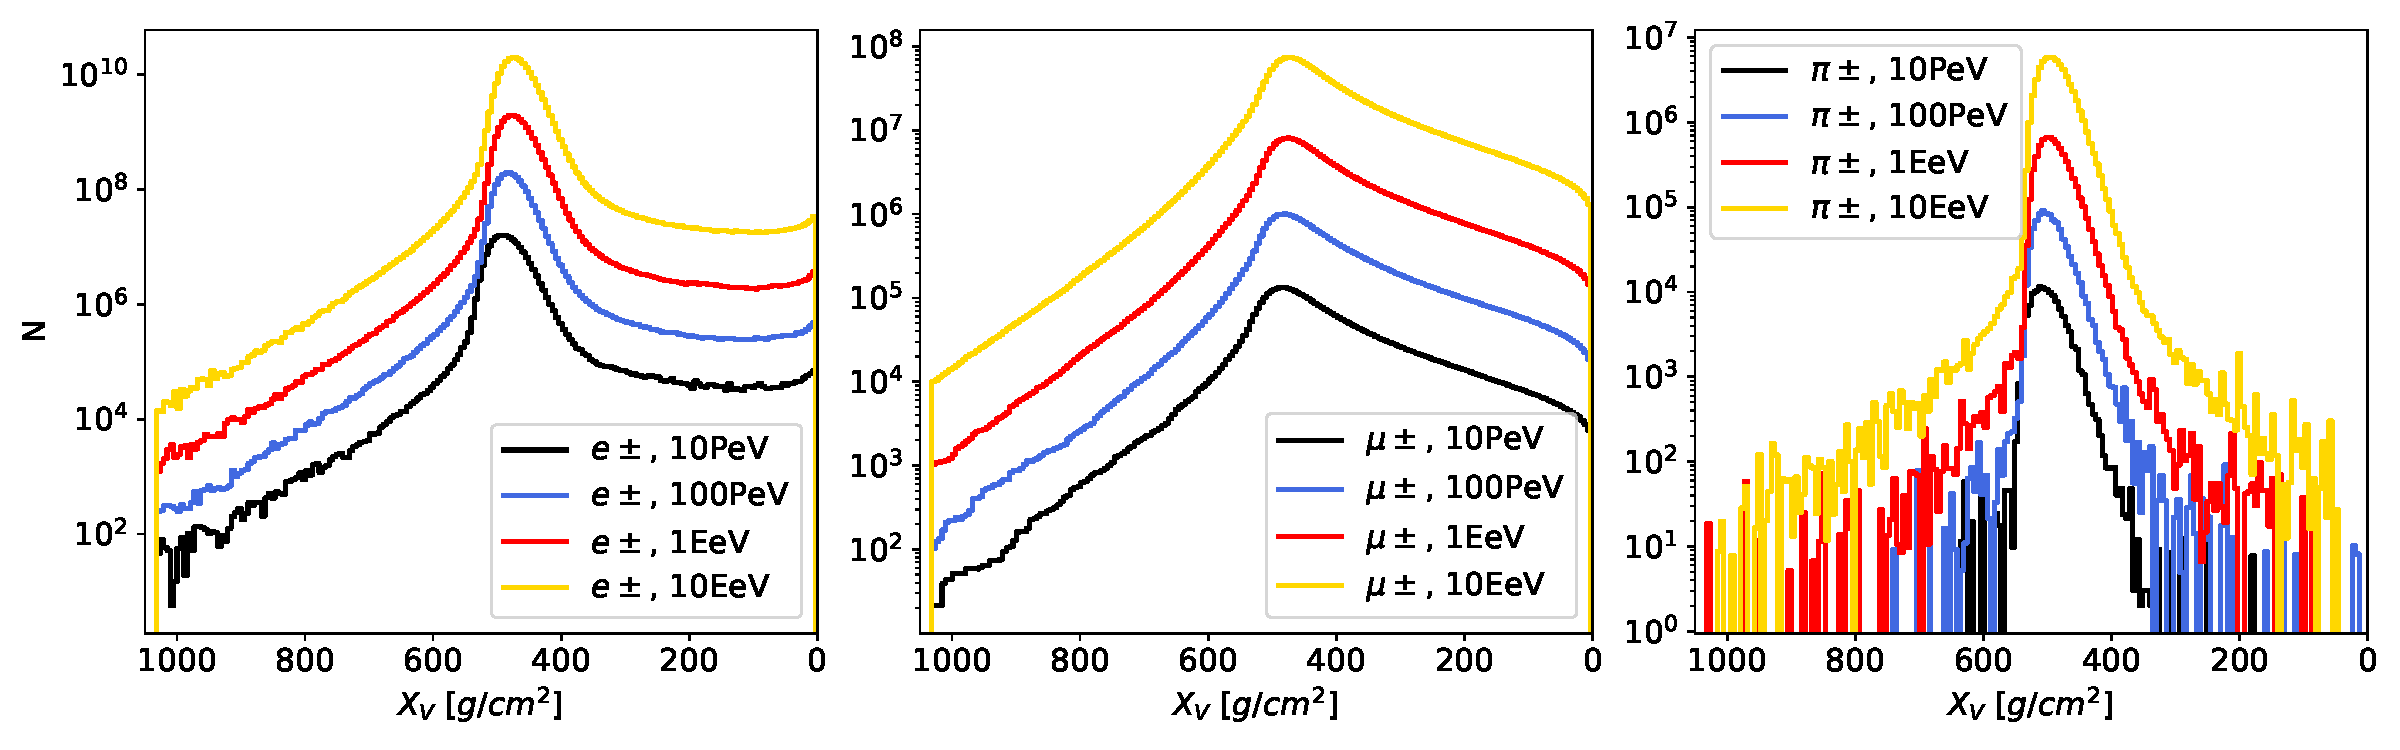
\includegraphics[width=1\linewidth]{figures/cascadas/upgoing_p_varE_95deg_5km_v2}
	\caption{Desarrollo de electrones, muones y piones en una cascada a $95^\circ$ iniciada por un protón de energía variable interaccionando a $5\,\mathrm{km}$ de altura.}
	\label{Carac_UG_varE}
\end{figure}
Como vemos, el número máximo de partículas producidas presenta una dependencia inequívoca con la energía del primario, $E_0$. De manera explícita, la tendencia que se espera tanto a partir de modelos teóricos como de simulaciones como las que hemos realizado es:
\begin{equation}
	N_{max}^{e}\propto E_0\;\;;\;\;N_{max}^{\mu}\propto E_0^\beta\;\text{con}\;\beta\sim0,85\label{ec25}
\end{equation}
Nuestro resultado, a simple vista, concuerda con esta tendencia (\textit{grosso modo}, aumentar $E_0$ en un factor 10 aumenta $N_{max}$ en un orden de magnitud). Más allá de lo anterior, las gráficas \ref{Carac_UG_varE} permiten mostrar claramente un efecto que habíamos mencionado: hacia el final de la cascada, aparecen cambios de pendiente en el desarrollo de $e^\pm$ y $\mu^\pm$ asociados a la desintegración de estos últimos.
\begin{itemize}
	\item \textit{Naturaleza del primario}
\end{itemize}
Hasta ahora, sólo hemos considerado cascadas iniciadas por un protón. Por ello, esta clase de cascadas presentan las tres componentes que discutimos al inicio de esta sección (electromagnética, hadrónica y muónica). Sin embargo, en cascadas iniciadas, por ejemplo, por un electrón o un fotón, no esperaríamos la aparición de componentes hadrónica o muónica, al menos no al mismo nivel que en cascadas iniciadas por protones o núcleos. Particularmente, en el caso que nos interesa podremos tener ambas situaciones, debido a los numerosos canales de desintegración del leptón $\tau$. Para estudiar esta clase de efectos, presentaremos a continuación resultados de simulaciones en AIRES en los que compararemos cascadas iniciadas por un protón o un electrón. Por simplicidad, y por ser un caso de particular interés dada la propuesta experimental que se planteó en la sec. \ref{sec1}, estudiaremos el caso de una cascada inclinada a $95^\circ$ iniciada por una partícula de $1\,\mathrm{EeV}$ que interacciona en las capas bajas de la atmósfera, a nivel del suelo:

\begin{figure}[H]
	\centering
	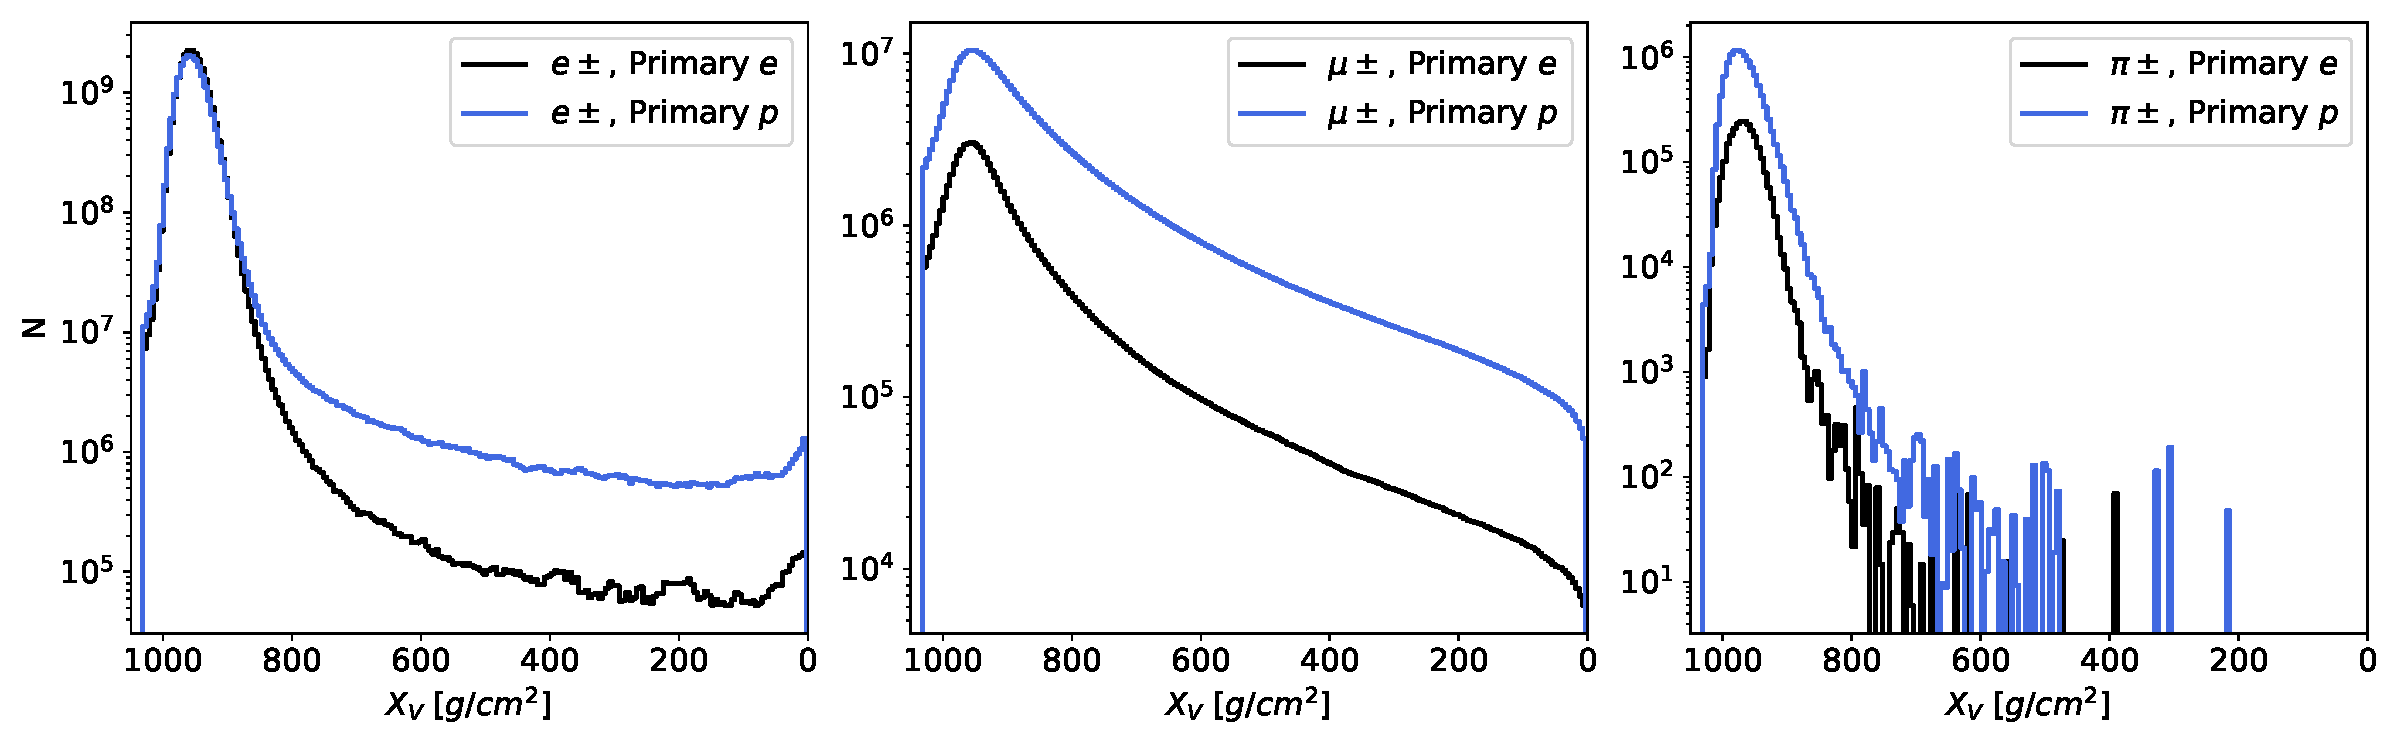
\includegraphics[width=1\linewidth]{figures/cascadas/upgoing_pe_1EeV_95deg_0km_v2}
	\caption{Desarrollo de electrones, muones y piones en una cascada a $95^\circ$ iniciada por un protón o un electrón de $1\,\mathrm{EeV}$ interaccionando a $0\,\mathrm{km}$ de altura}
	\label{Carac_UG_varprim}
\end{figure}

Como vemos inmediatamente, las cascadas iniciadas por protones presentan, respecto a una cascada iniciada por un electrón, un número de muones y piones superior en un factor $\sim 4$, aproximadamente. La diferencia no resulta demasiado grande, sobre todo recordando que los procesos que multiplican el número de piones (y por tanto de muones) al inicio de las cascadas requieren la presencia de hadrones de alta energía. Una explicación para esta observación es la presencia de reacciones fotonucleares, en las que un fotón de alta energía interacciona con un núcleo del medio produciendo hadrones ligeros. Dichos procesos tienen secciones eficaces muy inferiores a las de interacciones puramente hadrónicas\footnote{Típicamente dos órdenes de magnitud inferiores} y por tanto su contribución no se hace necesaria para interpretar las cascadas iniciadas por hadrones, aunque su efecto sí aparece cuando las interacciones hadrónicas no dominan, como en el caso de la cascada iniciada por electrón. 

 No obstante, el número máximo de electrones producido es similar en ambos casos. De nuevo, este es un reflejo del hecho de que, a lo largo del desarrollo de la cascada, existe una \textit{transferencia} de energía desde la componente hadrónica haca la componente electromagnética, fundamentalmente a través de la desintegración del pión neutro. Puesto que en ambos casos la energía del primario es la misma, el número de electrones y positrones producidos alcanza valores del mismo orden de magnitud. En el caso simulado de la Fig. \ref{Carac_UG_varprim} se encontró:
\begin{equation}
	\frac{N_e^{max}\;\;\text{(Prim. e)}}{N_e^{max}\;\;\text{(Prim. p)}}= 1,104 \label{ec26}
\end{equation}
El hecho de que se produzcan ligeramente menos electrones en la cascada iniciada por un protón de nuevo refleja el hecho de que una fracción de la energía del primario se encuentra en las componentes hadrónica y muónica. A pesar de todo, dado que $e^\pm$ son con diferencia las partículas más abundantes en cascadas atmosféricas, el número de partículas cargadas producidas en el máximo del desarrollo no tendrá una dependencia fuerte con la naturaleza del primario.

Por otra parte, observamos en la cascada iniciada por un protón que el número de electrones después de haber alcanzado el máximo es superior al que se observa en la cascada iniciada por un electrón, algo que puede resultar extraño ya que $N_{e}^{max}$ toma prácticamente el mismo valor en ambos casos.  

La razón para esta discrepancia reside precisamente en las contribuciones \textit{no electromagnéticas}. En una cascada iniciada por electrón, después de alcanzar el máximo del desarrollo los electrones producidos perderán energía con el medio, dando lugar a la caída que observamos en \ref{Carac_UG_varprim}. Sin embargo, en la cascada iniciada por un protón, tendremos muones que se propagarán sin interaccionar hasta decaer a mayor o menor altura, según su energía. Por ello, este mecanismo puede producir nuevos $e^\pm$ a mayores alturas, y su efecto es precisamente el que vemos en el desarrollo de electrones. 

Para verlo, podemos fijarnos simplemente en la proporción de partículas producidas en una cascada iniciada por protón relativa a una cascada iniciada por electrón (Fig. \ref{frac_primpe}). Como vemos, ambos cocientes se van al mismo valor después de haber alcanzado el máximo (obviando las fluctuaciones en los electrones, mucho más afectados por interacciones con el medio), lo que muestra que el exceso de electrones está relacionado con la mayor producción de muones. 
\begin{figure}[H]
	\centering
	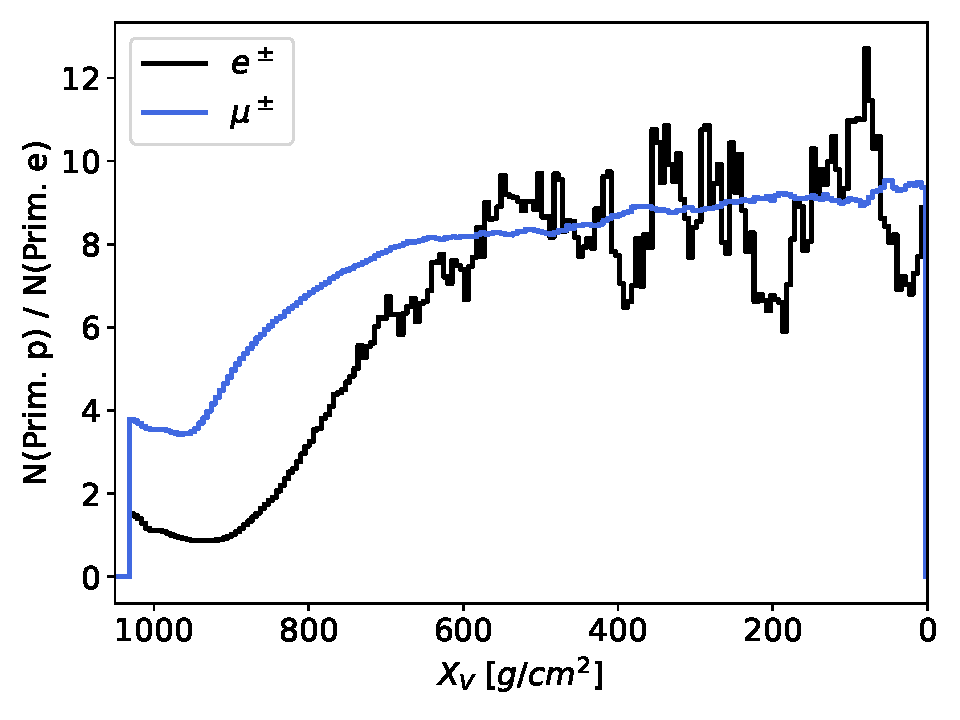
\includegraphics[width=.5\linewidth]{figures/cascadas/frac_emu_Primpe}
	\caption{Proporción entre $e^\pm$ ($\mu^\pm$) producidos en cascadas a $95^\circ$ iniciadas por un protón o electrón de $1\,\mathrm{EeV}$.}
	\label{frac_primpe}
\end{figure}

Otro observable que nos permitirá comprobar, al menos cualitativamente, que los muones originan los electrones \textit{extra} hacia el final del desarrollo es la evolución de su energía. En la sec. \ref{sec21} vimos cómo calcular la distancia que recorre una partícula antes de decaer en función de su energía \eqref{ec24}. Podemos invertir la relación para hallar la energía necesaria para recorrer una distancia $d$:
\begin{equation}
	E_{d} = \frac{mc^2}{c\tau} d\label{ec27}
\end{equation}
Por otra parte, en base a cálculos simples de geometría (Fig. \ref{evol_emu}a) y el modelo sencillo \eqref{ec21} podemos relacionar $d$ con $X_v$ en una cascada hacia arriba, y por lo tanto obtener la energía necesaria para alcanzar una profundidad $X_v$ sin decaer:
\begin{equation}
	\left.\begin{array}{r}d(h, \theta) =\sqrt{(R_T+h)^2-R_T^2\sin^2{\theta}}-R_T\cos{\theta}\\\\
	X_v=\int_h^\infty\rho(h')dh' \implies h(X_v) = h_0\log{\frac{\rho_0 h_0}{X_v}}\end{array}\right\}E_d(X_v, \theta) = \frac{mc^2}{c\tau}d(h(X_v),\theta)\label{ec28}
\end{equation}


\begin{figure}[H]
	\centering
	\subfigure[Geometría considerada \eqref{ec28}]{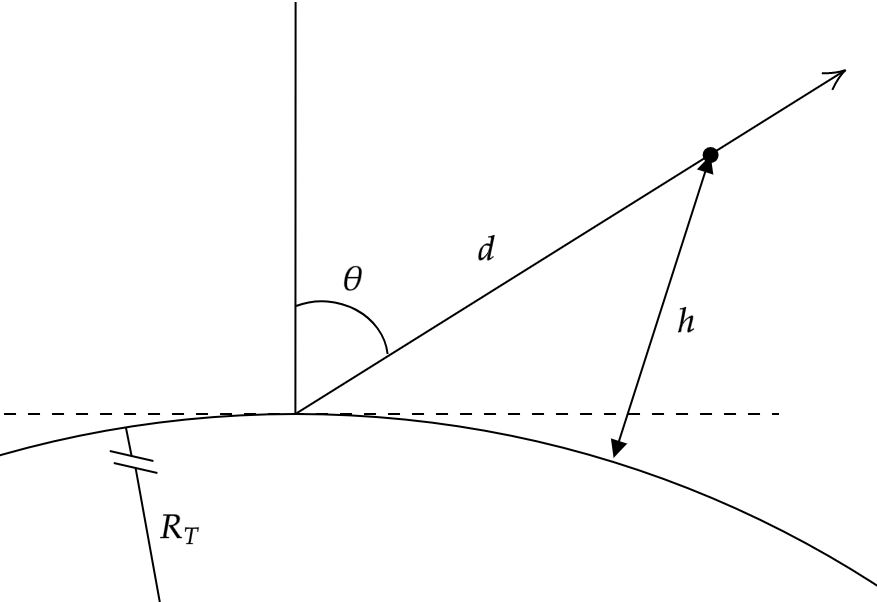
\includegraphics[width=0.45\linewidth]{figures/cascadas/sketch_evol_emu}}
	\hspace{10mm}
	\subfigure[Comparación de simulación con $E_d$]{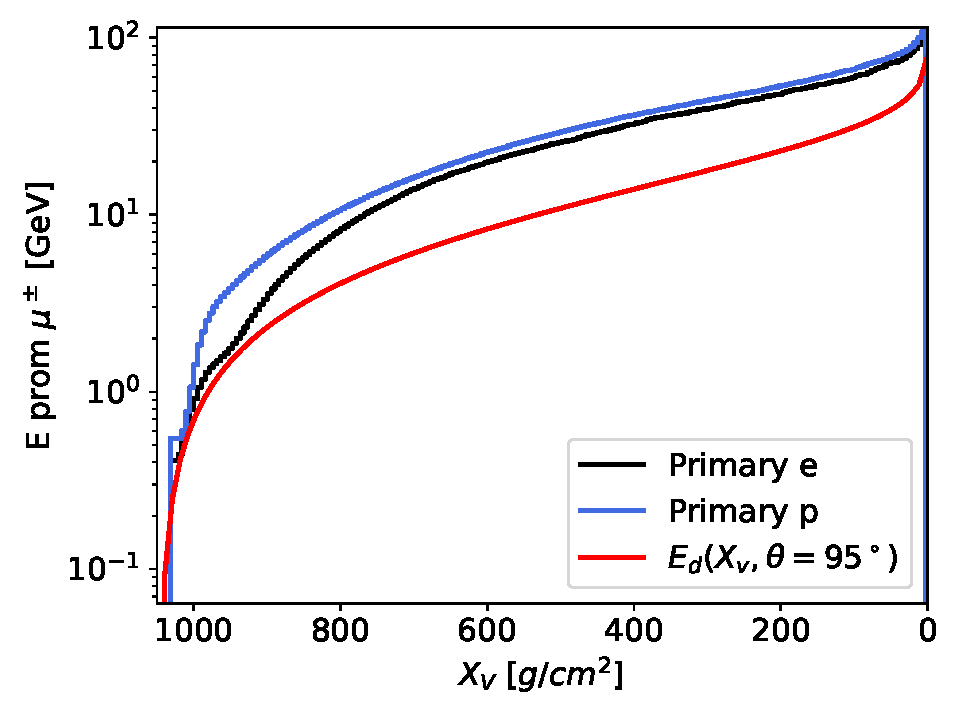
\includegraphics[width=0.45\linewidth]{figures/cascadas/evol_Emu_Primpe}}
	\caption{Evolución de la energía promedio por muón en una cascada a $95^\circ$.}
	\label{evol_emu}
\end{figure}
Como vemos, la evolución de la energía promedio sigue cualitativamente y en orden de magnitud el mismo comportamiento que la energía necesaria para alcanzar cierta altura en la atmósfera. La diferencia entre ambas curvas se debe a varios factores: en primer lugar, $E_d$ es la energía de un muón que se desintegra a una profundidad $X_v$, mientras que las simulaciones en AIRES precisamente muestran los muones que alcanzan un nivel de observación sin hacerlo (i.e., $E_d$ es una cota inferior a la energía). Por otra parte, hemos supuesto tanto un modelo muy simple de atmósfera como que todos los muones se producen en $h=0\,\mathrm{km}$. Además, la elección de $X_v$ como coordenada se ha hecho por ser posible obtener analíticamente\footnote{ La elección de $X_s$ o distancia a lo largo del eje podría ser más adecuada, aunque ambas requieren emplear cálculos numéricos. En el caso de $X_s$, la relación $d(X_s, \theta)$ debe obtenerse invirtiendo (para el modelo \eqref{ec21}):
$$X_s(d,\theta)=\int_{0}^{d}\rho(h(l))dl=\rho_0\int_{0}^{d}\exp\left[-\frac{1}{h_0}\left(\sqrt{(l+R_T\cos\theta)^2+R_T^2\sin^2\theta}\right)-R_T\right]dl$$ El resultado con esta elección no es sustancialmente distinto de \ref{evol_emu}. En el caso de trabajar con distancia a lo largo del eje, tenemos la desventaja de que AIRES sólo emplea profundidades como coordenadas, y la conversión a distancias se realiza numéricamente a posteriori.} la expresión \eqref{ec28}, pero tiene la desventaja de que podríamos \textit{mezclar} diferentes fases del desarrollo de la cascada (ver Fig. \ref{AIRES_planos}). En cualquier caso, la similitud del comportamiento entre la curva simulada y la que se obtiene de \eqref{ec27} y \eqref{ec28} de nuevo revela el papel de los muones como fuentes \textit{tardías} de electrones en cascadas hacia arriba.

Para finalizar la caracterización de cascadas hacia arriba, haremos una breve discusión acerca de las diferencias que aparecen en el desarrollo de las mismas comparadas con cascadas atmosféricas \textit{hacia abajo}, más estudiadas históricamente. Para ello, compararemos los resultados de AIRES para cascadas iniciadas por un protón de $1\,\mathrm{EeV}$ que interacciona a $0\,\mathrm{km}$ ($100\,\mathrm{km}$) de altura y con un ángulo de $\theta=95^\circ$ ($85^\circ$). Los resultados que discutiremos se presentan en las Figs. \ref{comp_ugdg} y \ref{comp_ugdg_vsd}:

\begin{figure}[H]
	\centering
	\subfigure[Número de partículas]{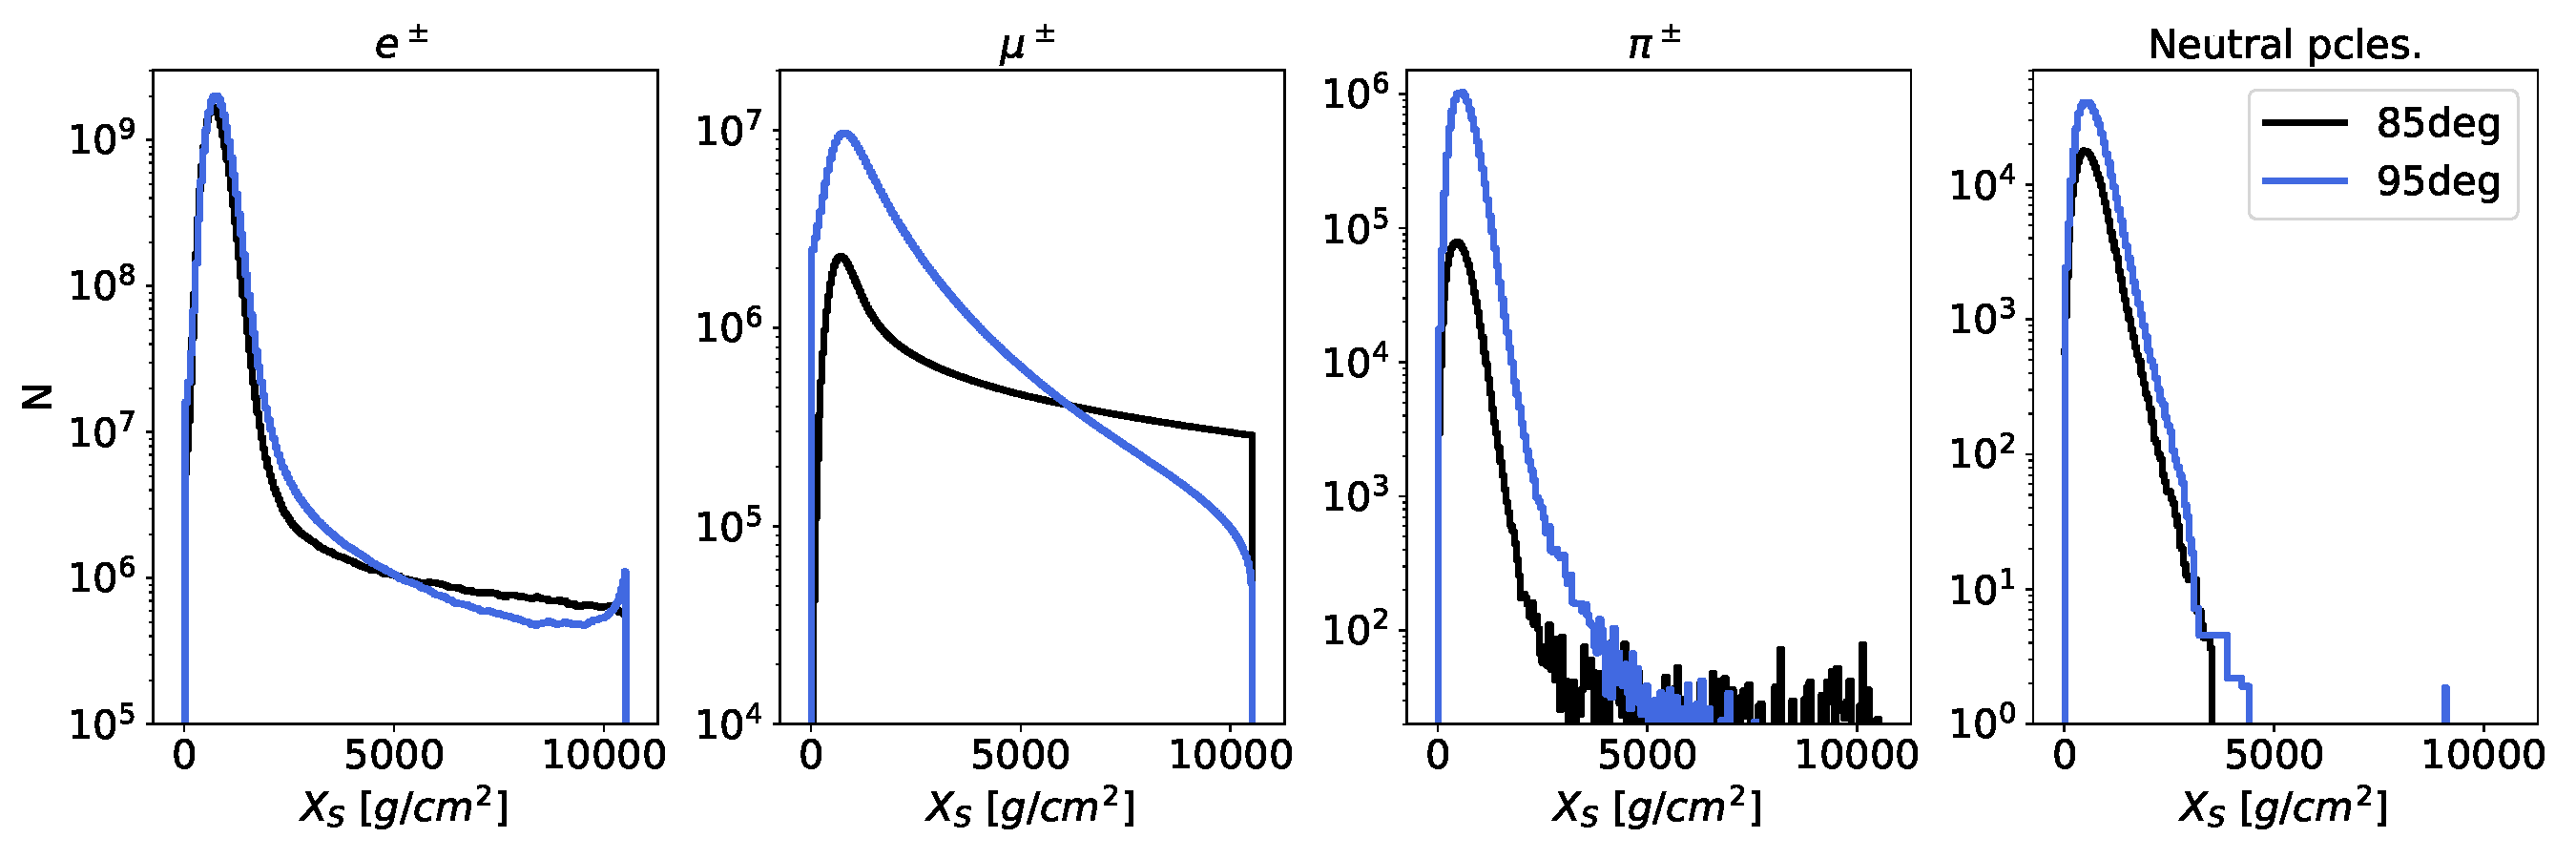
\includegraphics[width=1\linewidth]{figures/cascadas/comp_ugdg_number}}
	\\
	\subfigure[Energía promedio]{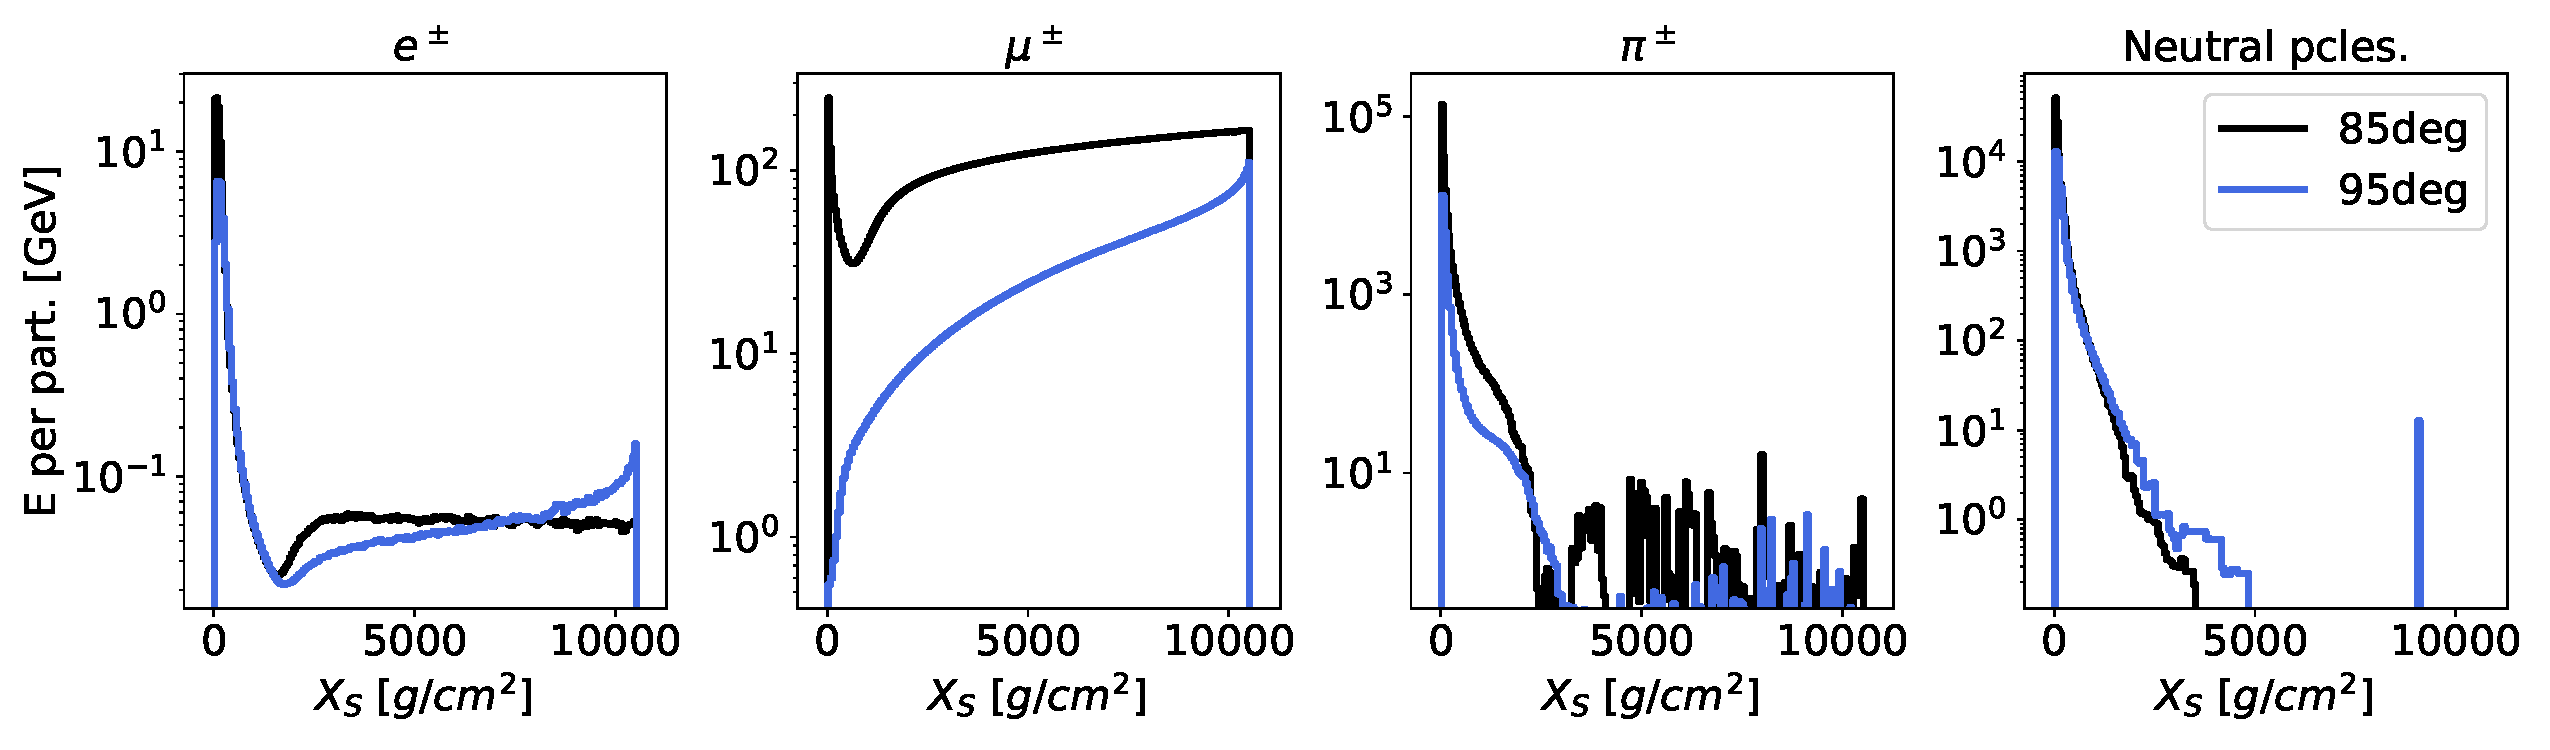
\includegraphics[width=1\linewidth]{figures/cascadas/comp_ugdg_egy}}
	\caption{Comparativa del desarrollo de cascadas hacia arriba y abajo, frente a profundidad atravesada (en la dirección del desarrollo). \textit{Neutral pcles.} engloba todas las partículas neutras producidas excepto neutrones.}
	\label{comp_ugdg}
\end{figure}

\begin{figure}[H]
	\centering
	\subfigure[Número de partículas]{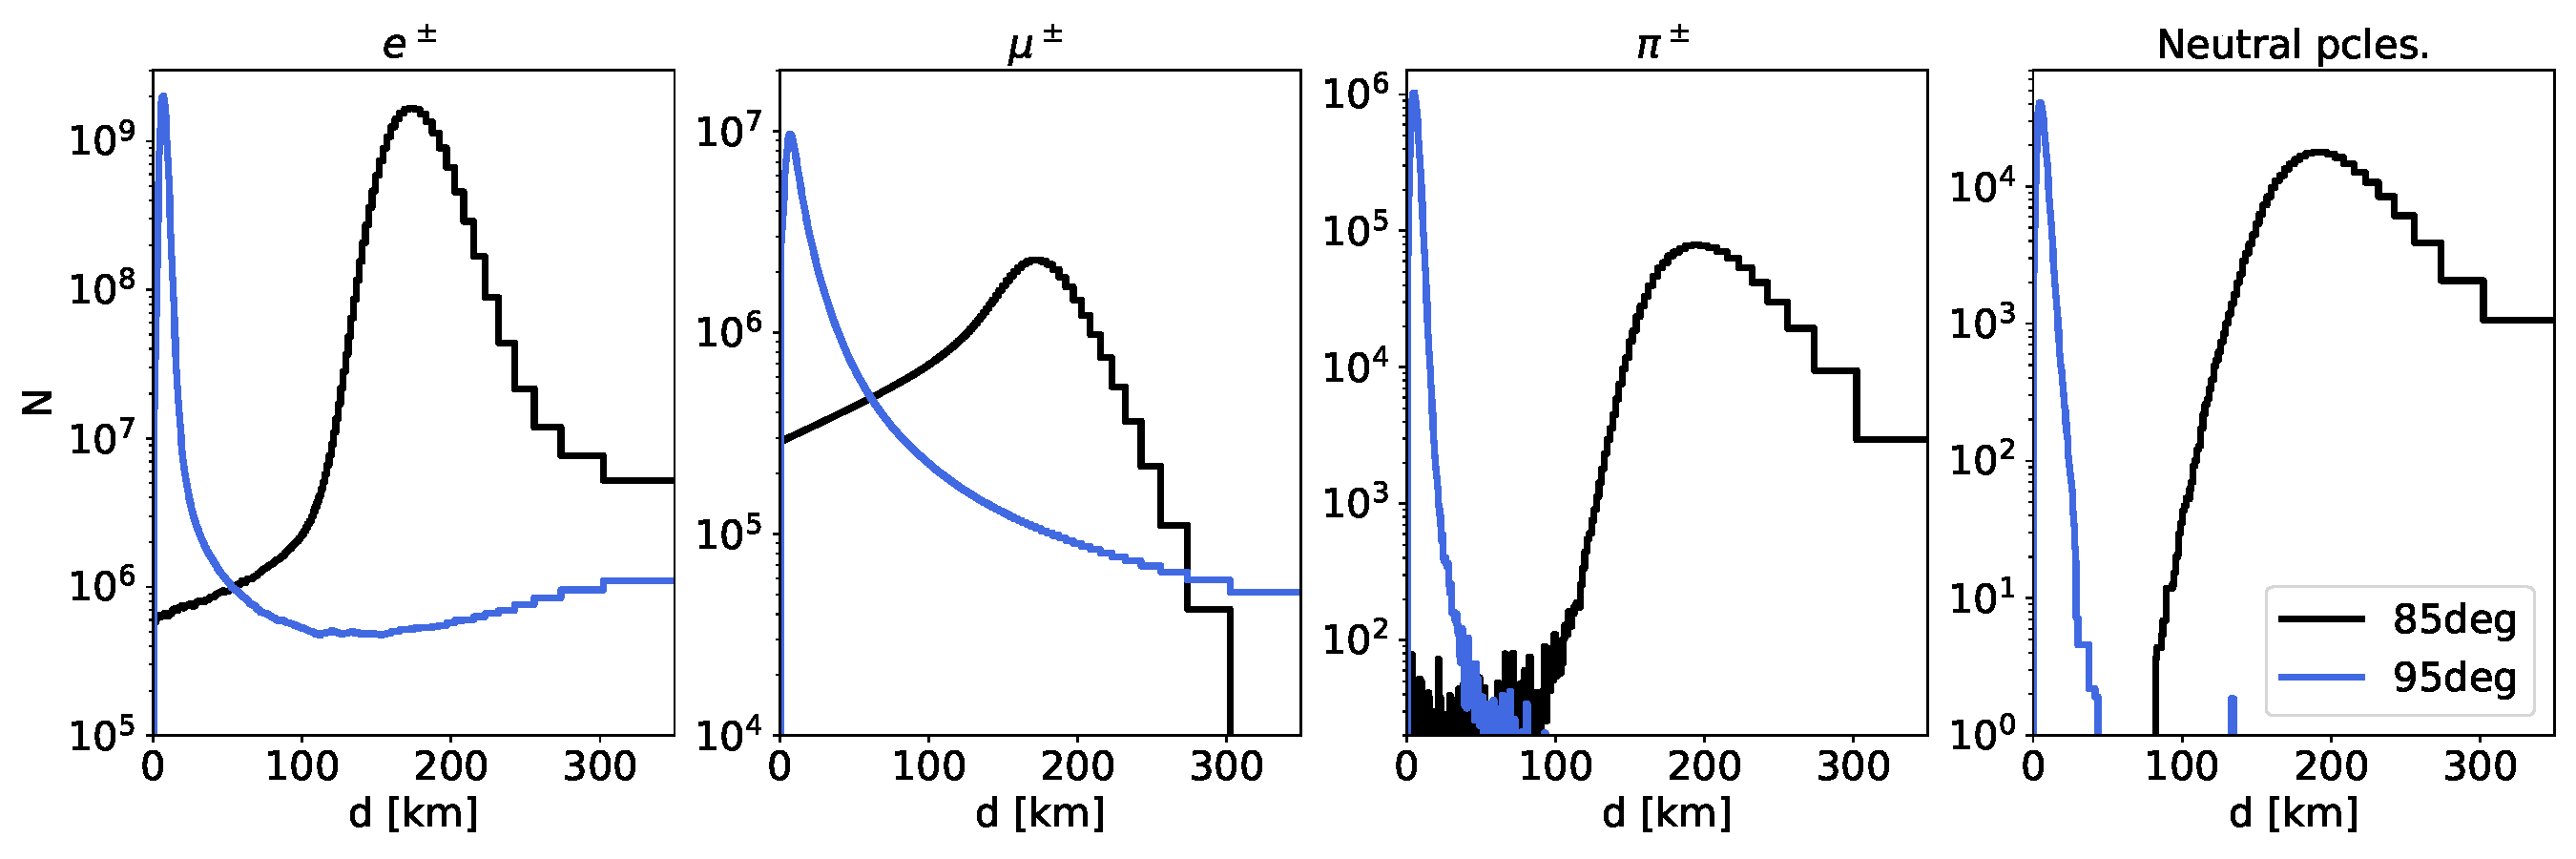
\includegraphics[width=1\linewidth]{figures/cascadas/comp_ugdg_number_vsd}}
	\\
	\subfigure[Energía promedio]{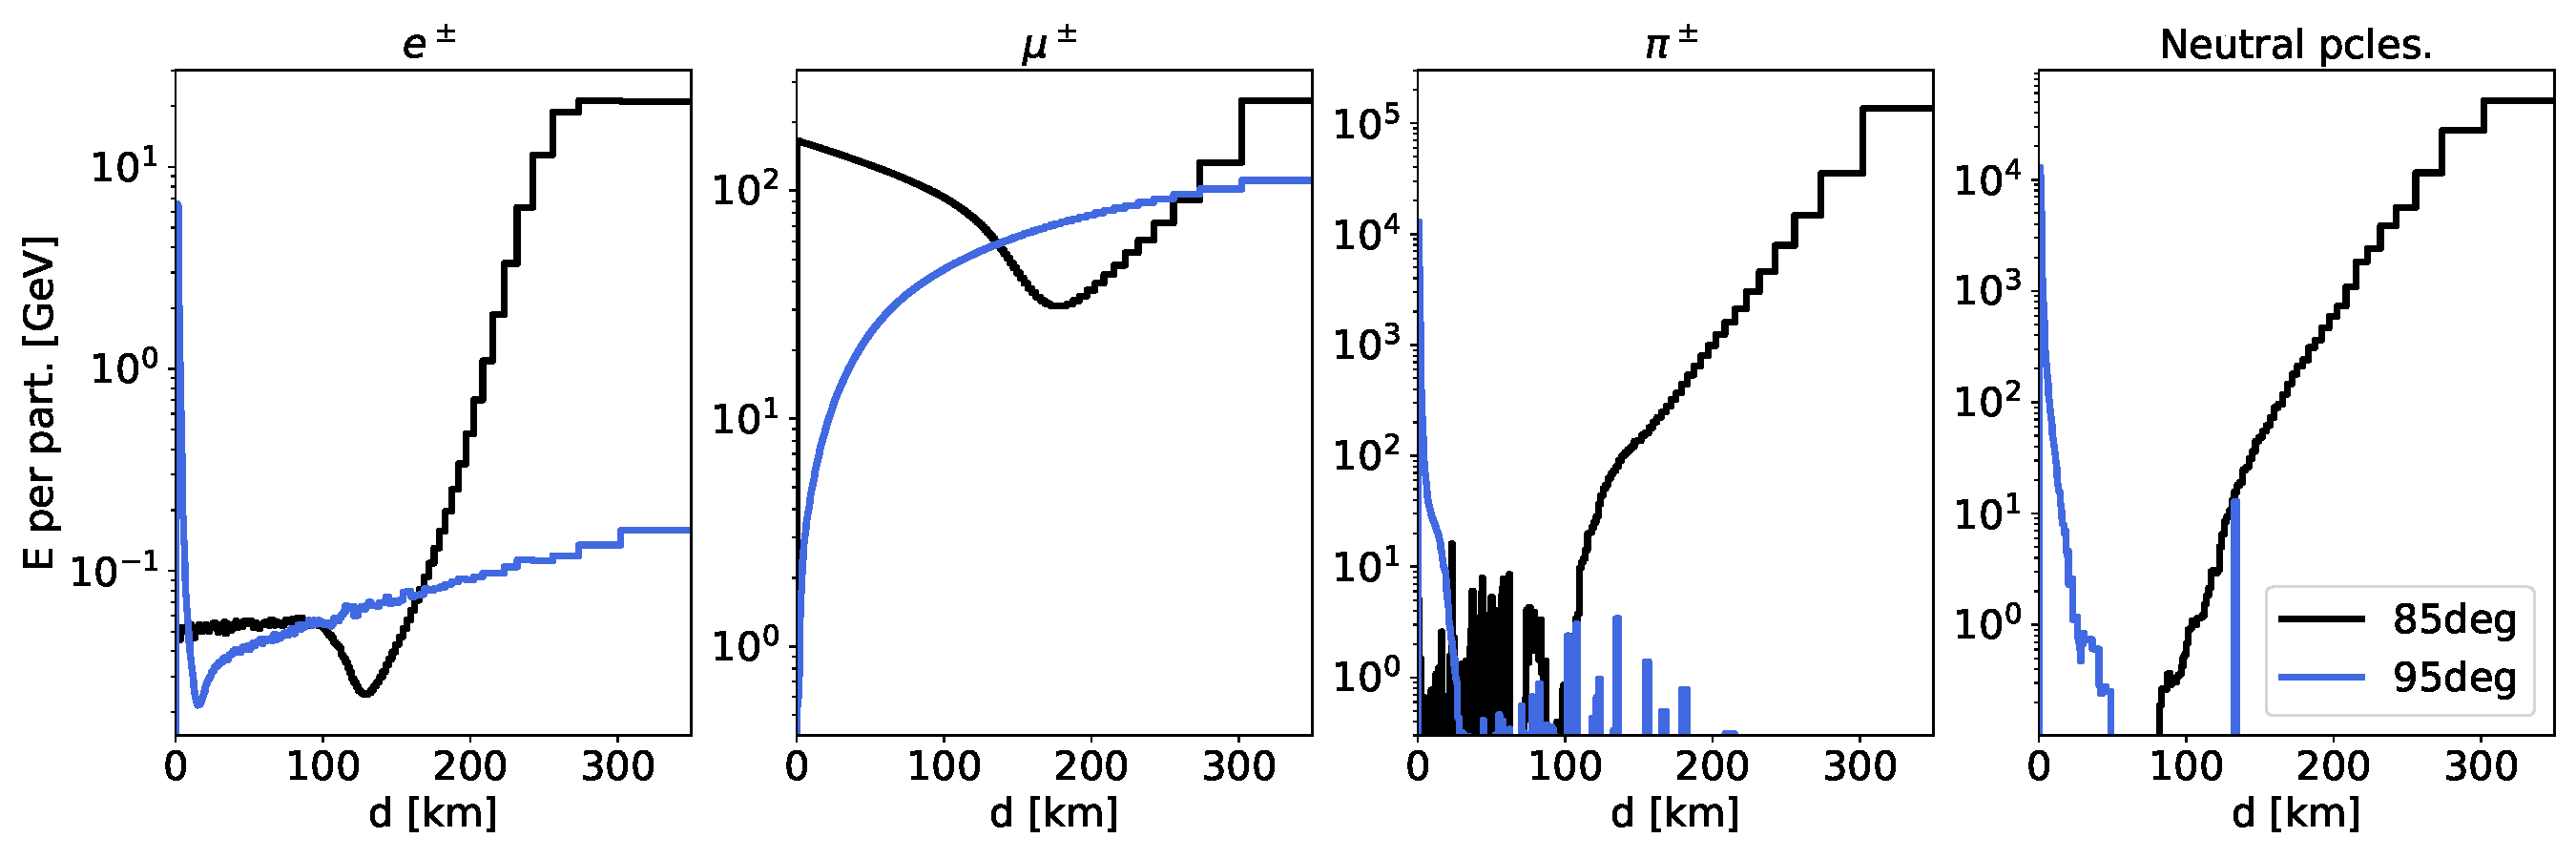
\includegraphics[width=1\linewidth]{figures/cascadas/comp_ugdg_egy_vsd}}
	\caption{Comparativa del desarrollo de cascadas hacia arriba y abajo, frente a distancia recorrida (en la dirección del desarrollo).}
	\label{comp_ugdg_vsd}
\end{figure}
Lo primero que observamos en las gráficas anteriores es la producción de un mayor número de partículas en el máximo en cascadas que \textit{viajan} hacia arriba. El efecto es especialmente claro en las gráficas que representan el desarrollo de muones y piones, aunque ocurre también para electrones. El origen de este comportamiento es precisamente el hecho de que la cascada hacia arriba se inicia en la región más densa de la atmósfera, en la que aparecen las partículas más energéticas del desarrollo y por tanto las interacciones que multiplican el número de partículas serán totalmente dominantes, mucho más que en cascadas hacia abajo en las que el desarrollo se inicia en zonas poco densas. Como hemos considerado cascadas iniciadas por protones, este efecto es especialmente visible en el desarrollo de piones cargados, y en los muones que se originan en las desintegraciones de los mismos. Por otra parte, si estudiamos el desarrollo en función de la distancia, vemos claramente que en cascadas hacia arriba el máximo ocurre prácticamente a nivel del suelo debido al elevado número de interacciones al inicio del desarrollo, frente a cascadas hacia abajo en que se requiere recorrer más distancia para atravesar la cantidad de materia necesaria para llegar al máximo. 

Si atendemos al desarrollo de la energía promedio por partícula, observamos que en cascadas hacia arriba las energías son menores que en el caso de cascadas hacia abajo. La razón para este comportamiento reside en el simple hecho de que, puesto que la energía del primario es la misma en ambos casos simulados, la producción de un mayor número de partículas en cascadas hacia arriba implica necesariamente que su energía debe ser menor. Precisamente por esto, la contribución de las desintegraciones aparecerá antes en cascadas hacia arriba. Dicho efecto es evidente en las gráficas de desarrollo de muones y piones cargados frente a distancia, también en la energía de los electrones (Fig. \ref{comp_ugdg_vsd}b). Como sabemos, la desintegración del muón aumentará la energía promedio de $e^\pm$ según avance el desarrollo. Vemos claramente que en cascadas hacia arriba el inicio de este crecimiento ocurre en menos tiempo, revelando que las desintegraciones comienzan a contribuir antes.

Por último, haremos un breve comentario acerca del desarrollo de las partículas neutras. Como sabemos, la contribución fundamental asociada en cascadas iniciadas por hadrones deberían ser los piones neutros. Como observamos, los desarrollos de partículas neutras, tanto en número como en energía, siguen un comportamiento similar al de $\pi^\pm$. Sin embargo, esperaríamos que $\pi^0$ y $\pi^\pm$ se produjeran en una proporción $1:2$, algo que no aparece en los desarrollos simulados. La razón para este hecho no es física sino que reside en el funcionamiento de AIRES y en la corta vida media del $\pi^0$, que hace que los piones neutros de menor energía se desintegren antes de alcanzar los niveles de observación establecidos\footnote{ En estas simulaciones se situaron 210 niveles de observación equiespaciados en $X_s$. Podemos estimar la distancia entre los planos como (ver ecs. \ref{ec21}, \ref{ec22}, \ref{ec24}): $$D \sim \frac{1}{210}\frac{X_s(100\,\mathrm{km}, 85^\circ)}{\rho_0}\sim \frac{1}{210}\frac{1000\,\mathrm{g/cm^2}}{\rho_0\cos85^\circ}\sim4\times 10^2\,\mathrm{m}\gg d_{dec}(\pi^0, 10^4\,\mathrm{GeV})\sim2\times10^{-3}\,\mathrm{m}$$}. No obstante, la similitud de ambas curvas revela que las partículas neutras que aparecen en cascadas atmosféricas tienen su origen en procesos hadrónicos.

Para terminar esta sección, recapitularemos algunos resultados relevantes:

\begin{enumerate}
	\item Las cascadas atmosféricas hacia arriba presentan un elevado número de partículas cargadas en el máximo ($\sim 10^8-10^{10}$), que a su vez aumenta con la inclinación de la cascada. 
	\item La altura de la primera interacción afecta a la posición del máximo en la atmósfera, aunque no influye demasiado en el número total de partículas cargadas producidas (siempre que la primera interacción no ocurra por encima de las decenas de $\mathrm{km}$)
	\item La energía del primario está altamente relacionada con el número máximo de partículas producidas en cascadas atmosféricas, manteniendo una dependencia prácticamente lineal.
	\item La naturaleza hadrónica o leptónica se refleja en el desarrollo tardío de la cascada, en que los electrones aparecen \textit{retardados} debido a la contribución muónica. La diferencia en el número máximo de partículas entre ambos casos es pequeña comparada con el efecto de la energía del primario.
	\item Las cascadas hacia arriba presentan máximos muy localizados en las proximidades del nivel del suelo y con una elevada producción de partículas, comparadas con cascadas hacia abajo.
\end{enumerate}
\clearpage %cleardoublepage pode meter paxinas en branco. Non e obrigatorio. Tampouco para a 
	\section{Emisión en radio: Principio físico y caracterización}\label{sec3}
	Uno de los objetivos fundamentales de este trabajo, como hemos comentado en el apartado introductorio, es la caracterización de las radiofrecuencias emitidas en cascadas atmosféricas y el estudio de su posible aprovechamiento para la detección de neutrinos tau de origen astrofísico. Para poder avanzar en esta cuestión, primero presentaremos los mecanismos físicos que originan dicha emisión, ya que una buena comprensión de los mismos es, como poco, importante para poder interpretar los resultados posteriores.
	\subsection{Formalismo de la emisión}\label{sec31}
	Como es bien sabido, la presencia de cargas en movimiento en un determinado medio implica, casi de manera inevitable, la emisión de radiación. Resulta entonces evidente que, en una cascada atmosférica iniciada, por ejemplo, por un protón o un neutrino de origen astrofísico en la que aparecerán un número gigantesco de partículas cargadas propagándose con una velocidad $v\sim c$, podemos esperar la aparición de radiación electromagnética.
	
	Ahora bien, uno podría pensar a priori que, en las escalas de energía y número de partículas que involucra una cascada atmosférica, el balance \textit{macroscópico} de cargas positivas y negativas debería ser nulo, y por lo tanto las respectivas contribuciones a la radiación electromagnética emitida deberían cancelarse. Sin embargo, existen dos aspectos acerca del desarrollo de una cascada en la atmósfera que inmediatamente nos obligan a abandonar esta perspectiva ingenua:
	\begin{itemize}
		\item En primer lugar, la cascada se desarrolla en presencia del campo magnético terrestre, y por lo tanto las cargas sufren una deflexión en un sentido u otro según el signo de su carga. En una perspectiva \textit{macroscópica}, podemos interpretar que este efecto origina una corriente neta perpendicular tanto al desarrollo de la cascada como al campo magnético terrestre, generando entonces un campo eléctrico.
		\item En segundo lugar, la cascada no se desarrolla en el vacío sino en presencia de materia. Aunque en la cascada se produzca globalmente el mismo número de partículas con carga positiva que negativa, las interacciones con el medio darán lugar a un exceso de carga. Por ejemplo, los positrones generados en la cascada sufrirán procesos de aniquilación con los electrones del medio. Por otra parte, estos mismos electrones del medio podrán ser extraídos por diversos procesos (scattering $e^-e^-$, difusión Compton, ...) y contribuirán también a la aparición de una corriente neta. 
	\end{itemize}

Estos dos mecanismos, a los que a partir de ahora nos referiremos como \textit{deflexión geomagnética} y \textit{efecto Askaryan}\footnote{ Este mecanismo de emisión fue propuesto por Gurgen A. Askaryan en la década de los 60.} respectivamente, serán los procesos que darán lugar fundamentalmente a la emisión coherente de radiación electromagnética en cascadas atmosféricas.

Para ahondar en los mecanismos de emisión, recordaremos brevemente algunos conceptos de la electrodinámica clásica que nos permitirán explicar, al menos de manera cualitativa, los campos eléctricos que esperamos a partir de cada mecanismo. Partiremos de las ecuaciones de Maxwell en términos de los potenciales:
	\begin{equation}
	\vect{\nabla}^2\phi+\frac{\partial}{\partial t}\left(\vect{\nabla}\cdot\vect{A}\right)=-\frac{\rho}{\varepsilon}\label{ec31}
	\end{equation}
	\begin{equation}
	\vect{\nabla}^2\vect{A}-\mu\varepsilon\frac{\partial^2\vect{A}}{\partial t^2}-\vect{\nabla}\left(\vect{\nabla}\cdot\vect{A}+\mu\varepsilon\frac{\partial^2\phi}{\partial t^2}\right)=-\mu\vect{J}\label{ec32}
	\end{equation}

Por la libertad gauge, escogemos $\vect{\nabla}\cdot \vect{A}=0$ (gauge de Coulomb). En ese caso, los potenciales electromagnéticos toman la forma\footnote{ Véase por ejemplo \cite{Jackson2002}.} ($\vect{R}=\vect{r}-\vect{r}'$):
\begin{equation}
	\phi(\vect{r}, t)=\frac{1}{4\pi\varepsilon}\int_{\text{fuente}} \frac{\rho(\vect{r}', t)}{\left|\vect{R}\right|}d^3r'\label{ec33}
\end{equation}
\begin{equation}
	\vect{A}\left(\vect{r}, t\right)=\frac{\mu}{4\pi}\int_{\text{fuente}}\frac{\left[\vect{J}\left(\vect{r}', t_{ret}\right)-\left(\vect{J}\left(\vect{r}', t_{ret}\right)\cdot \hat{\vect{R}}\right)\hat{\vect{R}}\right]}{\left|\vect{R}\right|}d^3r'+\mathcal{O}(\left|\vect{R}\right|^{-3})\label{ec34}
\end{equation}
donde\footnote{ $n$ es el índice de refracción del medio.} $t_{ret}=t-nR/c$, y en \eqref{ec34} se desprecian términos que no contribuyen en la región de radiación. Las expresiones anteriores, aunque no sean especialmente simples de manejar, nos permitirán caracterizar los dos mecanismos de emisión que hemos comentado, sin más que tener en cuenta que:
\begin{itemize}
	\item En este gauge, el potencial escalar $\phi$ viene dado por una solución \textit{instantánea}, en el sentido de que no hay ninguna dependencia con $t_{ret}$. La consecuencia inmediata es que $\phi$ sólo describe efectos de campo cercano, y podremos escribir sencillamente:
	\begin{equation}
		\vect{E}=-\vect{\nabla}\phi-\dot{\vect{A}}\implies \vect{E}_{rad} = -\dot{\vect{A}}\label{ec35}
	\end{equation}
\item La solución para el potencial vector depende exclusivamente de la componente \textit{perpendicular} a $\vect{R}$ de la corriente:
\begin{equation}
	\vect{J}=\vect{J}_\parallel+\vect{J}_\perp = \left(\vect{J}\cdot\hat{\vect{R}}\right)\hat{\vect{R}}-\hat{\vect{R}}\times\left(\hat{\vect{R}}\times\vect{J}\right)\label{ec36}
\end{equation} 
Por lo tanto, el breve desarrollo anterior nos permite establecer que el campo eléctrico radiado tendrá la dirección de la componente perpendicular\footnote{Estrictamente, de su derivada temporal. En los mecanismos de emisión considerados, $\vect{J}\parallel \dot{\vect{J}}$ aproximadamente.} $\vect{J}_\perp$ de la corriente generada por cada mecanismo:
\begin{equation}
	\left.
	\begin{array}{c}
		\vect{E}_{rad} = -\dot{\vect{A}}\\
		\vect{A}\sim\vect{J}_\perp=-\hat{\vect{R}}\times\left(\hat{\vect{R}}\times\vect{J}\right)
	\end{array}
\right\}\vect{E}_{rad}\parallel  \hat{\vect{R}}\times\left(\hat{\vect{R}}\times\vect{J}\right)\label{ec37}
\end{equation}
\end{itemize}
Este último resultado es suficiente para estudiar la polarización del campo eléctrico generado por una cascada atmosférica, bien por deflexión geomagnética o por efecto Askaryan. Por simplicidad, consideremos una cascada que se desarrolla en la dirección vertical (i.e. con un ángulo cenital $\theta=0^\circ$). El efecto de la deflexión geomagnética está determinado por la acción de la fuerza de Lorentz sobre las cargas generadas:
\begin{equation}
	\vect{F}=q\vect{v}\times \vect{B}\implies \vect{J}\sim \hat{\vect{n}}_{\text{shower}}\times\vect{B}\label{ec38}
\end{equation}
donde $\hat{\vect{n}}_{\text{shower}}$ representa la dirección del desarrollo de la cascada. El efecto puede verse más claramente en la Fig. \ref{Geomag_deflexion}, en donde también representamos la polarización del campo radiado mediante este mecanismo.

\newpage
\begin{figure}[H]
	\centering
	\subfigure[]{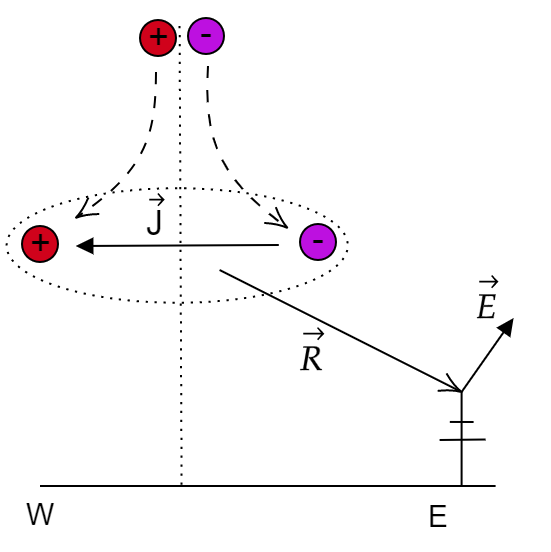
\includegraphics[width=0.3\linewidth]{figures/Geomag_deflexion_1}}
	\hspace{10mm}
	\subfigure[]{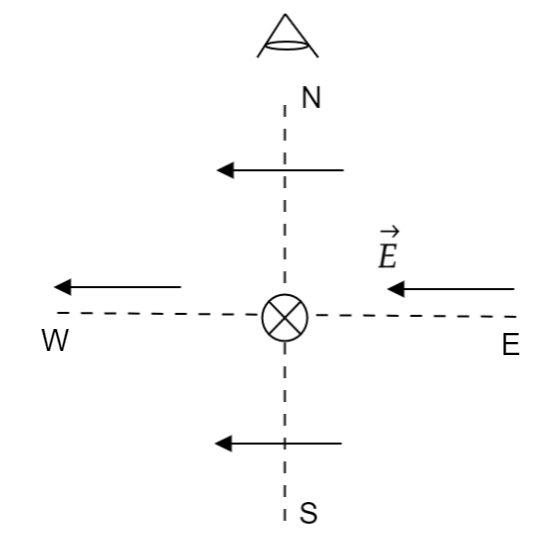
\includegraphics[width=0.3\linewidth]{figures/Geomag_deflexion_2}}
	\caption{Campo eléctrico radiado por efecto de la deflexión geomagnética. (a) Dirección del campo $\vect{E}_{rad}\parallel  \hat{\vect{R}}\times\left(\hat{\vect{R}}\times\vect{J}\right)$ en una antena prueba al oeste de una cascada vertical. (b) Dirección esperada para el campo eléctrico radiado en una cascada vertical (se indica la posición del observador de la Fig. a). Las direcciones N, S, E, W hacen referencia al polo norte magnético.}
	\label{Geomag_deflexion}
\end{figure}

Si queremos hacer el mismo análisis para el efecto Askaryan, la polarización del campo radiado ahora estará determinada por el exceso de carga que aparece a lo largo del desarrollo. Naturalmente, las partículas más abundantes en una cascada atmosférica serán electrones y positrones, tanto por ser las especies de menor masa como por existir numerosos mecanismos que los originan. Como ya mencionamos, los positrones desaparecerán en procesos de aniquilación, mientras que otros electrones del medio serán extraídos y contribuirán a la carga neta generada. Por ello, el efecto Askaryan se traduce en la aparición de un exceso de carga negativa a lo largo del desarrollo y por tanto:
\begin{equation}
	\vect{J}\sim -\hat{\vect{n}}_{\text{shower}}\label{ec39}
\end{equation}
La polarización del campo generado por este mecanismo se representa en la Fig. \ref{Askaryan} para una cascada vertical. Como vemos, expresiones sencillas como \eqref{ec37}, \eqref{ec38} y \eqref{ec39} son suficientes para describir cualitativamente el campo eléctrico radiado por una cascada de dirección arbitraria.
\begin{figure}[H]
	\centering
	\subfigure[]{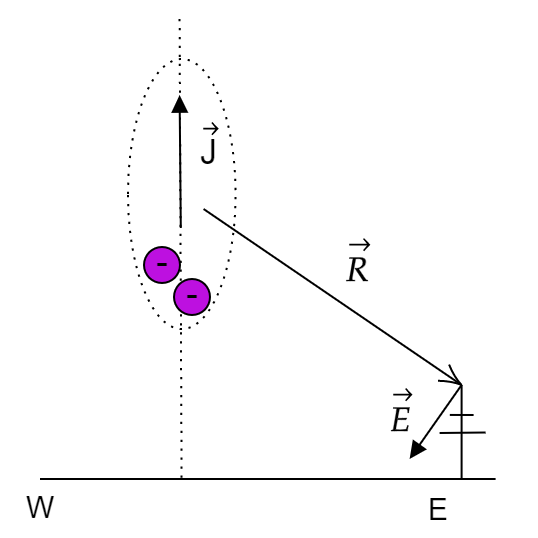
\includegraphics[width=0.3\linewidth]{figures/Askaryan_1}}
	\hspace{10mm}
	\subfigure[]{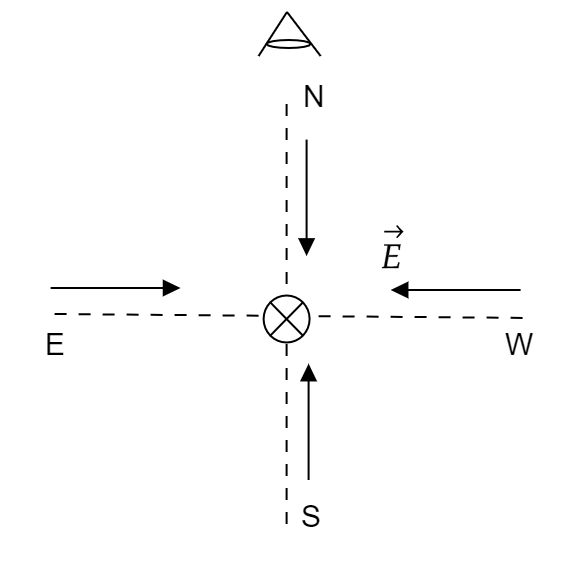
\includegraphics[width=0.3\linewidth]{figures/Askaryan_2}}
	\caption{Campo eléctrico radiado por efecto Askaryan. Mismos gráficos que en la Fig \ref{Geomag_deflexion}.}
	\label{Askaryan}
\end{figure}

Hasta ahora, hemos hecho una descripción \textit{macroscópica} de la emisión de radiación electromagnética, en el sentido de que hemos considerado la aparición de corrientes netas como un efecto global sobre la cascada. Aunque este enfoque es muy intuitivo y permite explorar las características de la emisión, un análisis detallado de la misma deberá realizarse desde una perspectiva \textit{microscópica}, i.e. considerando la radiación emitida por partículas cargadas de manera \textit{individual}. Dado que este es el marco en el que se desarrollan nuestras simulaciones, y también porque nos permitirá extraer alguna conclusión extra acerca de la emisión, estudiaremos algo más esta perspectiva. Para empezar, reescribamos el potencial vector \eqref{ec34}:
\begin{equation}
	\vect{A}\left(\vect{r}, t\right)=\frac{\mu}{4\pi}\int \frac{\vect{J}_\perp\left(\vect{r}', t'\right)}{\left|\vect{R}\right|}\,\delta\left(\frac{n}{c}\left|\vect{R}\right|-\left(t-t'\right)\right)d^3r'dt'\label{ec310}
\end{equation} 
donde sólo hemos introducido una función-$\delta$ que evalúa la corriente en $t_{ret}$. Supongamos ahora una carga puntual $q$ que se mueve a velocidad constante $\vect{v}$, entre $t=t_1$ y $t=t_2$. La corriente $\vect{J}$ asociada puede escribirse fácilmente:
\begin{equation}
	\vect{J}_\perp\left(\vect{r'}, t'\right)=q\vect{v}_\perp \,\delta^{(3)}\left(\vect{r}'-\vect{r}_0-\vect{v}t'\right)\left[\Theta\left(t'-t_1\right)-\Theta\left(t'-t_2\right)\right]\label{ec311}
\end{equation}
donde $\vect{r}_0=\vect{r}'\left(t=0\right)$, y el último término son funciones de Heaviside que garantizan que $\vect{J}_\perp=0$ para $t<t_1$ ó $t>t_2$. Sustituyendo esta última expresión en \eqref{ec310} e integrando en $d^3r'$ (aplicando la función-$\delta^{(3)}$), tenemos que:
\begin{equation}
	\vect{A}\left(\vect{r}, t\right)=\frac{\mu q}{4\pi}\vect{v}_\perp\int \frac{\delta\left(\frac{n}{c} \left|\vect{r}-\vect{r}_0-\vect{v}t'\right|-\left(t-t'\right)\right)}{\left|\vect{r}-\vect{r}_0-\vect{v}t'\right|}\left[\Theta\left(t'-t_1\right)-\Theta\left(t'-t_2\right)\right]dt'\label{ec312}
\end{equation}
A grandes distancias, en el régimen de Fraunhofer, podemos escribir:
\begin{equation}
	\left|\vect{r}-\vect{r}_0-\vect{v}t'\right|\approx R-t'\vect{v}\cdot\hat{\vect{R}}\;\;;\;\;\frac{1}{\left|\vect{r}-\vect{r}_0-\vect{v}t'\right|} \approx \frac{1}{R}\label{ec313}
\end{equation}
Sustituyendo estas aproximaciones en \eqref{ec312} y aplicando propiedades de las funciones $\delta$ y $\Theta$, es fácil obtener:
\begin{equation}
	\vect{A}\left(\vect{r}, t\right)\approx\frac{\mu q}{4\pi R}\vect{v}_\perp\frac{\Theta\left[t-nR/c-\left(1-n\beta\cos{\theta}\right)t_1\right]-\Theta\left[t-nR/c-\left(1-n\beta\cos{\theta}\right)t_2\right]}{1-n\beta\cos{\theta}}\label{ec314}
\end{equation}
donde hemos usado que $\left|\vect{v}\right|=\beta c$, además de definir el ángulo de observación como $\cos{\theta}=\hat{\vect{v}}\cdot\hat{\vect{R}}$. Como comentamos anteriormente, el campo eléctrico en este régimen puede obtenerse derivando \eqref{ec314} respecto a $t$:
\begin{equation}
	\vect{E}\left(\vect{r}, t\right)\approx-\frac{\mu q}{4\pi R}\vect{v}_\perp\frac{\delta\left[t-nR/c-\left(1-n\beta\cos{\theta}\right)t_1\right]-\delta\left[t-nR/c-\left(1-n\beta\cos{\theta}\right)t_2\right]}{1-n\beta\cos{\theta}}\label{ec315}
\end{equation}

De lo anterior puede extraerse fácilmente la expresión para el campo eléctrico en el dominio de frecuencias, sin más que hacer una transformada de Fourier\footnote{ Se ha usado el criterio (poco común) de transformada de Fourier empleado en el algoritmo ZHS (ver siguiente apartado):
	$$\tilde{f}(\omega)=2\int dt \exp\left(i\omega t\right)f(t)$$}:
\begin{equation}
	\vect{E}\left(\vect{r}, \omega\right)\approx-\frac{\mu q}{2\pi R}\vect{v}_\perp \exp\left(i\omega\frac{nR}{c}\right)\frac{e^{i\omega(1-n\beta\cos{\theta})t_1}-e^{i\omega(1-n\beta\cos{\theta})t_2}}{1-n\beta\cos{\theta}}\label{ec316}
\end{equation}
Podríamos preocuparnos acerca del hecho de que lo que hemos obtenido es el campo eléctrico radiado por una partícula moviéndose a $\vect{v}$ constante, i.e., sin aceleración. Sin embargo, las funciones-$\delta$ de la expresión anterior implican que sólo existe una contribución no nula en los extremos de la trayectoria (recordemos que la partícula \textit{aparece} en $t_1$ y \textit{desaparece} en $t_2$, véase la ec. \ref{ec311}), mientras que a lo largo de la trayectoria no se emite radiación, como esperaríamos.

Más allá del comentario anterior, podemos extraer dos conclusiones importantes en lo que sigue:
\begin{itemize}
	\item En primer lugar, el campo eléctrico presenta una divergencia cuando el ángulo de observación coincide con el ángulo \v{C}erenkov del medio, $\cos{\theta_C}=1/n\beta$. Aunque esta divergencia es fruto de las aproximaciones del cálculo, describe correctamente el hecho de que el \textit{pico} de las emisiones se localiza en $\theta=\theta_C$. El resultado es natural, en una cascada se producirán partículas viajando a $v\sim c$, más rápido que la luz en la atmósfera ($n\geq 1$) y por lo tanto el valor máximo del campo eléctrico radiado aparecerá asociado al cono \v{C}erenkov.
	\item En segundo lugar, y desde un punto de vista más técnico, las expresiones \eqref{ec315} y \eqref{ec316} pueden incorporarse fácilmente a cálculos numéricos y simulaciones del desarrollo de cascadas.
\end{itemize}

Precisamente el último punto resulta de especial interés en este trabajo, ya que nuestro último objetivo será caracterizar la emisión de radio en cascadas atmosféricas hacia arriba mediante simulaciones. En el siguiente apartado nos detendremos en el algoritmo empleado en las mismas, y mostraremos algunos resultados sencillos que nos permitirán poner en contexto el desarrollo que hemos realizado en este apartado.

	\subsection{Simulación y caracterización de la radiación}\label{sec32}

Las simulaciones de la emisión electromagnética asociada a cascadas atmosféricas se ha realizado recurriendo al código ZHAireS, que combina la simulación del desarrollo de cascadas atmosféricas mediante AIRES con el algoritmo ZHS \cite{AlvarezMuniz2012, Zas1992} para calcular el campo eléctrico radiado. El desarrollo de la sección anterior será suficiente para describir, al menos de manera cualitativa, el funcionamiento de dicho algoritmo:
	\begin{itemize}
		\item Las trayectorias de las partículas son discretizadas en \textit{sectores}, en los cuales la velocidad de la partícula se toma constante. Los parámetros de cada sector (energía, dirección, ...) se obtienen de AIRES.
		\item En cada paso de la simulación, la partícula se propagará a lo largo de un \textit{sector}, entre $t$ y $t+\Delta t$. Introduciendo las posiciones de observación (antenas) en la simulación, las expresiones \eqref{ec315} y \eqref{ec316} permiten calcular el campo eléctrico asociado al sector, tanto en dominio temporal como de frecuencias.
		\item Si en algún sector no se verifican las condiciones del régimen de Fraunhofer (e.g. trayectorias muy cercanas a una antena), dicho sector podrá subdividirse en \textit{subsectores} hasta alcanzar dimensiones lo suficientemente pequeñas para poder aplicar las expresiones \eqref{ec315} y \eqref{ec316}.
		%En cascadas atmosféricas, las dimensiones típicas de las mismas son comparables a la distancia a las antenas ($\sim 10^{2-3}\,\mathrm{m}$). Para evitar abandonar el 

		
	\end{itemize}
Mediante esta técnica, puede simularse el campo eléctrico radiado por una cascada atmosférica en función del tiempo o la frecuencia, sin más que acumular la contribución de todas las partículas consideradas en cada paso de la simulación. Además, las expresiones \eqref{ec315} y \eqref{ec316} se extraen directamente de principios básicos, sin suponer un mecanismo de emisión u otro. Por ello, este algoritmo tiene inmediatamente en cuenta la emisión de radiación asociada a la (des)aparición de partículas cargadas en el medio y a las interacciones consideradas, así como efectos de interferencia al sumar las contribuciones de cada partícula. En la Fig. \ref{ZHSsketch} mostramos esta idea:  
	\begin{figure}[H]
		\centering
		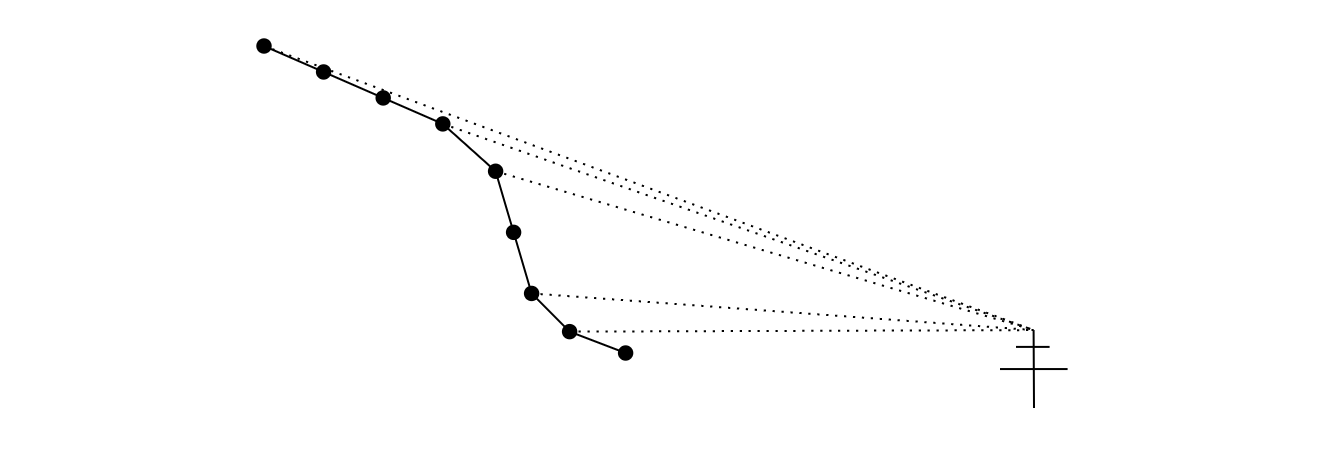
\includegraphics[width=.8\linewidth]{figures/ZHSsketch}
		\caption{Idea básica del algoritmo ZHS. La trayectoria de las partículas se discretiza, permitiendo aplicar expresiones como \eqref{ec315} de manera sencilla.}
		\label{ZHSsketch}
	\end{figure}
 
Mostraremos ahora algunos ejemplos de resultados típicos de ZHAireS, que nos permitirán poner de manifiesto algunas de las ideas desarrolladas hasta el momento. El primer caso que planteamos es el de una cascada vertical ($\theta=0^\circ$) iniciada por un protón de energía inicial $E=10^{17}\,\mathrm{eV}$. El campo magnético terrestre se ha supuesto, por simplicidad, horizontal (i.e., paralelo al plano del suelo) y de magnitud $23\,\mathrm{\mu T}$, y se han situado antenas en las cuatro direcciones relativas al \textit{core} de la cascada (N, S, E, W). Los resultados de la simulación se presentan en las Figs. \ref{EW_field} y \ref{NS_field}. Aunque a simple vista no es evidente, dichos resultados son un ejemplo perfecto para ver los efectos de los mecanismos de emisión que discutimos en la sec. \ref{sec31}. 

Empecemos por la Fig. \ref{EW_field}, en la que presentamos la componente $y$ del campo eléctrico, i.e., la componente en la dirección Este-Oeste (EW). Como vemos, la forma de la señal es muy similar en todas las posiciones, con un pulso de duración $\sim \mathrm{ns}$ cuya amplitud decrece con la distancia al \textit{core} de la cascada. Sin embargo, aparece una diferencia muy interesante en los máximos: tanto en las antenas al Norte y Sur se alcanzan los mismos valores aproximadamente, mientras que en las antenas al Este (Oeste) se llega a valores algo superiores (inferiores). En este efecto es donde podemos apreciar la competición entre la deflexión geomagnética y el efecto Askaryan. Recordando las Figs. \ref{Geomag_deflexion} y \ref{Askaryan}, es evidente que el efecto Askaryan no modifica de manera sustancial la componente $y$ del campo si nos situamos al Norte o al Sur, mientras que aporta una contribución que se añade (resta) al campo generado por deflexión geomagnética al Este (Oeste). Por ello, el campo observado en el Este es ligeramente superior al del Oeste, mientras que este efecto no aparece en observaciones al Norte o Sur.


\begin{figure}[H]
	\centering
	\subfigure[Norte]{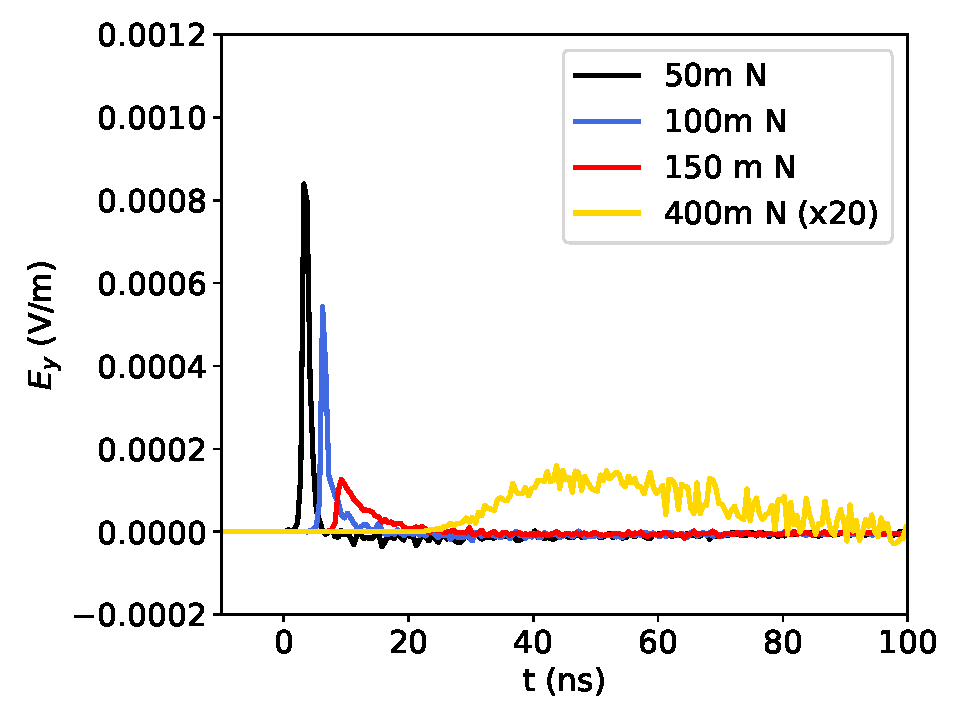
\includegraphics[width=0.45\linewidth]{figures/radio/p_1e17_0deg_EW_N_v2}}
	\subfigure[Sur]{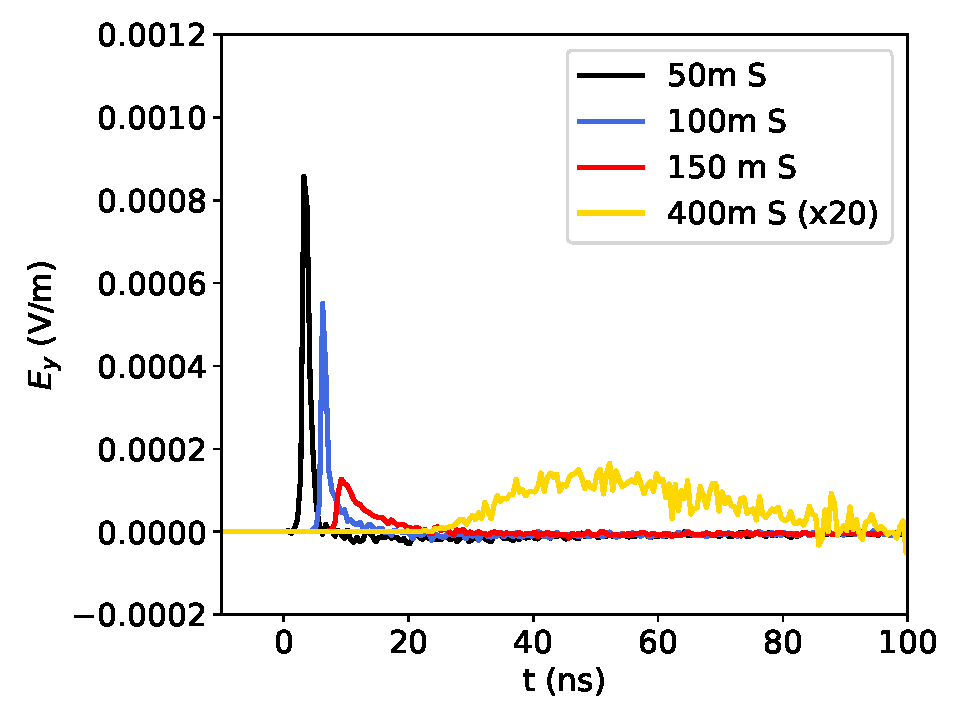
\includegraphics[width=0.45\linewidth]{figures/radio/p_1e17_0deg_EW_S_v2}}
	\\
	\subfigure[Este]{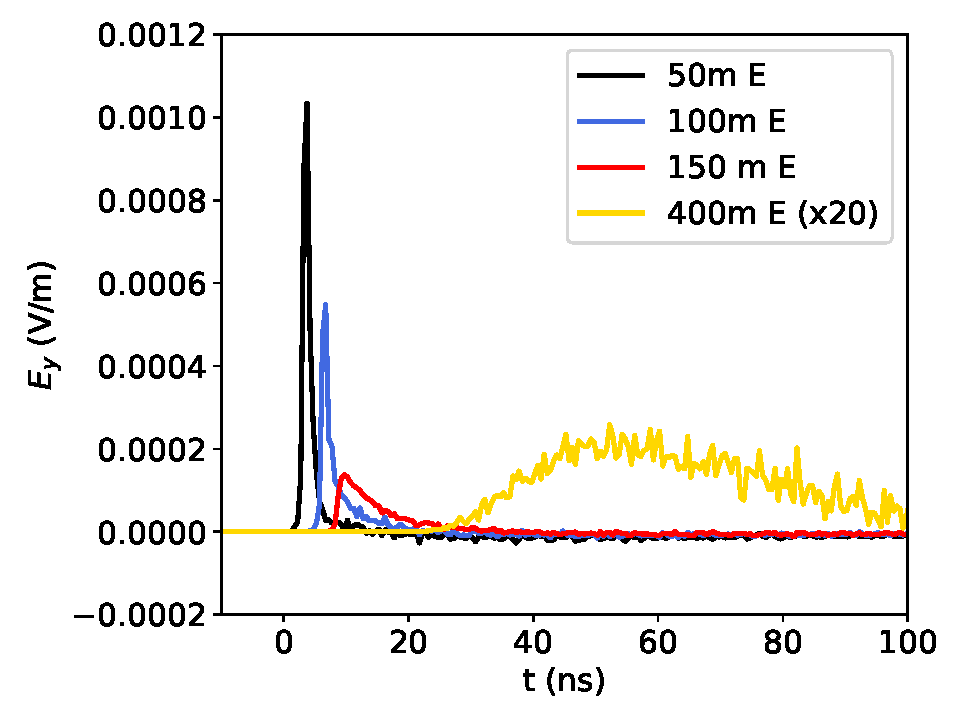
\includegraphics[width=0.45\linewidth]{figures/radio/p_1e17_0deg_EW_E_v2}}
	\subfigure[Oeste]{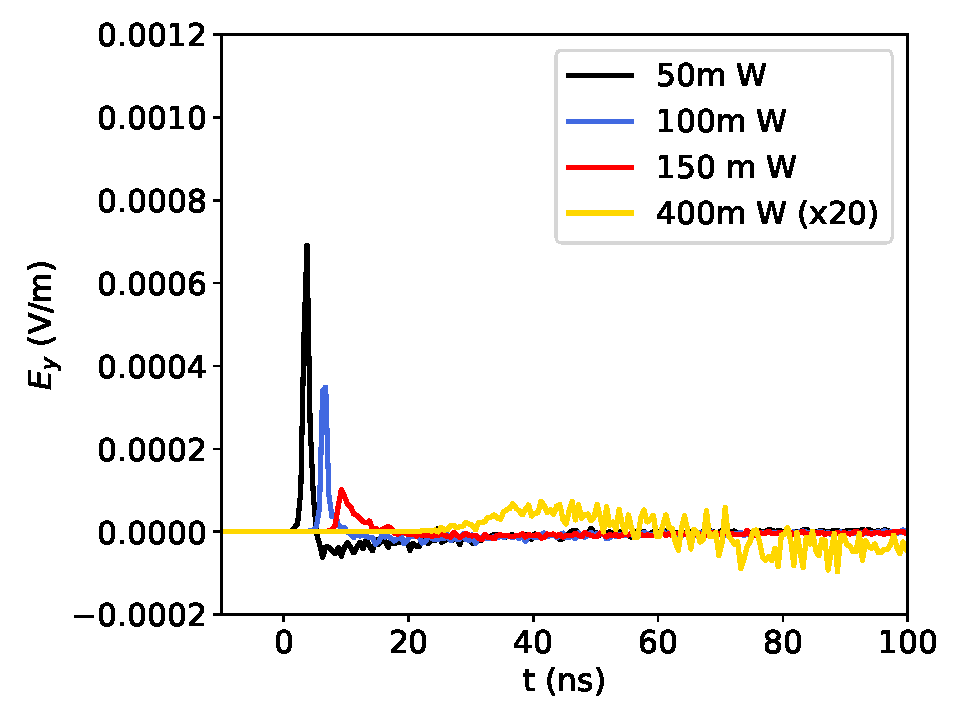
\includegraphics[width=0.45\linewidth]{figures/radio/p_1e17_0deg_EW_W_v2}}
	\caption{Componente $y$ (E$\rightarrow$W) del campo eléctrico radiado por una cascada vertical iniciada por un protón de $10^{17}\,\mathrm{eV}$, en diferentes puntos de observación. La señal a $400\,\mathrm{m}$ se ha multiplicado por un factor $20$ para hacerla visible.}
	\label{EW_field}
\end{figure}

Si nos centramos en la componente $x$ del campo, es decir, en la dirección Norte-Sur (NS), es evidente a partir de las Figs. \ref{Geomag_deflexion} y \ref{Askaryan} que sólo \textit{veremos} el efecto Askaryan en antenas al Norte y Sur, mientras que la deflexión geomagnética no será relevante. Además, esperamos que dicha componente NS del campo tenga signo opuesto. Precisamente, este es el resultado que observamos en la Fig. \ref{NS_field}. Además, por simetría (Fig. \ref{Askaryan}), podemos suponer que la \textit{contribución Askaryan} a la componente $x$ del campo en antenas al N,S ($\sim 2\times10^{-4}\,\mathrm{V/m}$) será igual a la contribución al campo en la dirección $y$ en antenas al E,W. Como vemos, dicho valor es plenamente coherente con que la diferencia que observábamos en las antenas E,W en la Fig. \ref{EW_field} tenga su origen en el efecto Askaryan.
\begin{figure}[H]
	\centering
	\subfigure[Norte]{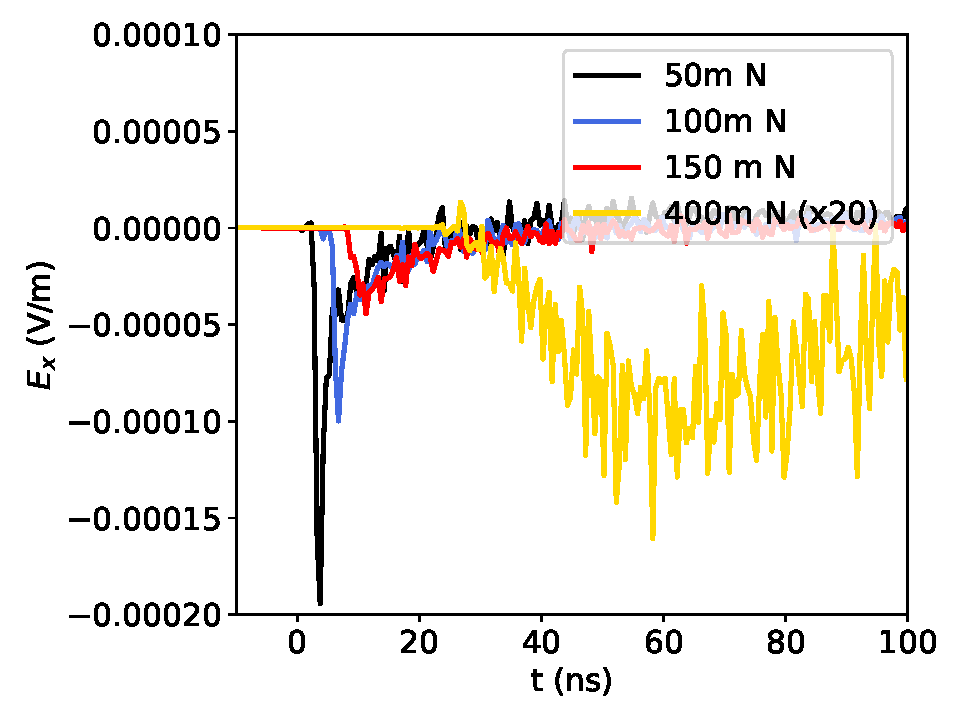
\includegraphics[width=0.45\linewidth]{figures/radio/p_1e17_0deg_NS_N_v2}}
	\subfigure[Sur]{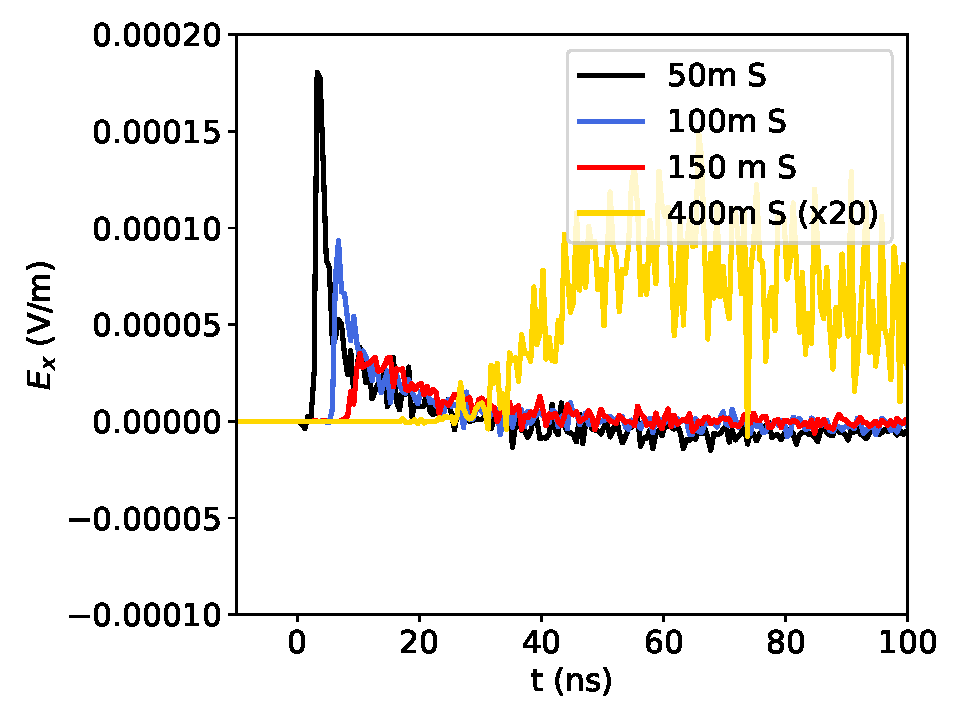
\includegraphics[width=0.45\linewidth]{figures/radio/p_1e17_0deg_NS_S_v2}}
	\\
	\subfigure[Este]{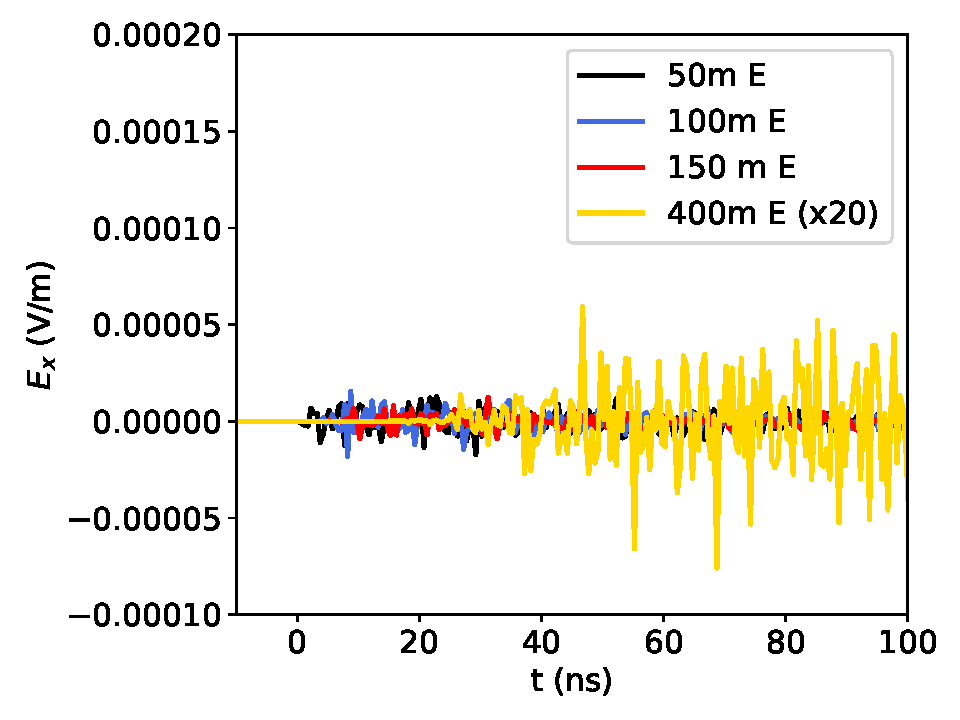
\includegraphics[width=0.45\linewidth]{figures/radio/p_1e17_0deg_NS_E_v2}}
	\subfigure[Oeste]{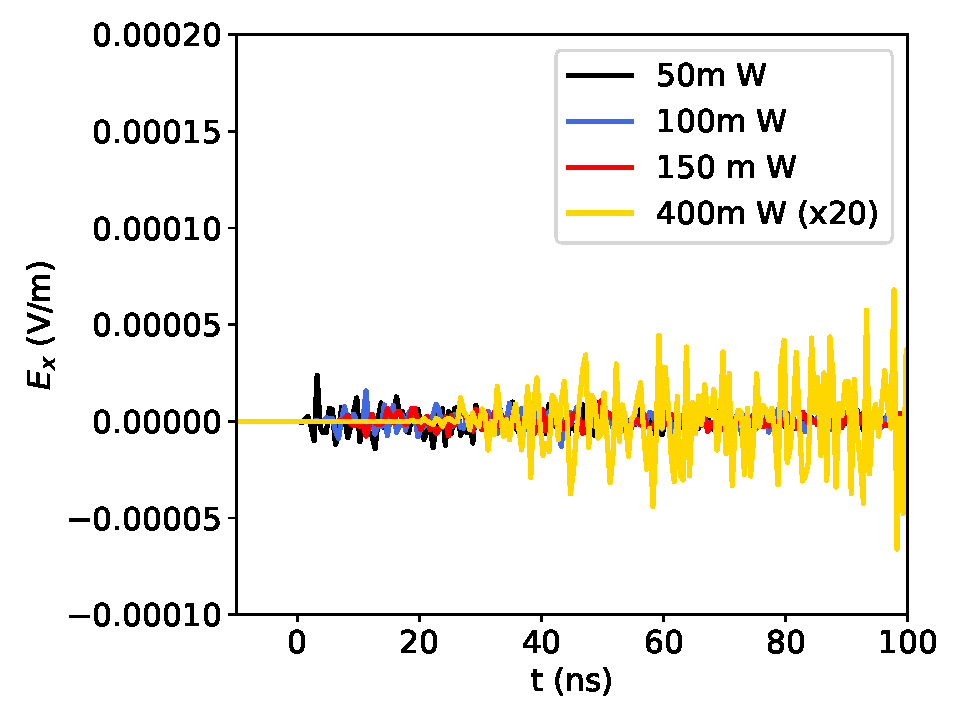
\includegraphics[width=0.45\linewidth]{figures/radio/p_1e17_0deg_NS_W_v2}}
	\caption{Equivalente a Fig. \ref{EW_field} para la componente $x$ (S$\rightarrow$N) del campo.}
	\label{NS_field}
\end{figure}
A partir de estos resultados, podemos plantearnos la pregunta de \textit{qué} banda de frecuencias será de interés a la hora de estudiar la emisión electromagnética en cascadas atmosféricas. El enfoque más directo para responder a esa pregunta es estudiar la transformada de Fourier de las señales en tiempo. Por ello, presentamos como ejemplo en la Fig. \ref{E_fields_FFT} el campo eléctrico en el dominio de frecuencias\footnote{ Aplicando una transformación de Fourier rápida (FFT) a la señal en tiempo simulada, sin recurrir al output de ZHAireS en frecuencias.} correspondiente a las Figs. \ref{EW_field}a y \ref{NS_field}a. Como vemos, el espectro mantiene un comportamiento \textit{suave} hasta aproximadamente $10-100\,\mathrm{MHz}$, en que la coherencia de la señal desaparece. Por ello, podemos adelantar que la banda de interés estará entre las decenas y centenas de $\mathrm{MHz}$, i.e., en las radiofrecuencias. Una justificación muy simple a que la emisión se produzca de manera coherente en esta banda de frecuencia puede hacerse en términos de un modelo geométrico muy sencillo, representando la cascada como un frente de partículas de cierta anchura y \textit{grosor}. Como vemos en la Fig. \ref{coherence}, a un observador a gran distancia (en el régimen de Fraunhofer) llegarían señales con retardos debidos al desarrollo longitudinal, lateral y al propio grosor del frente.

\begin{figure}[H]
	\centering
	\subfigure[Componente $y$ del campo, al Norte de la cascada.]{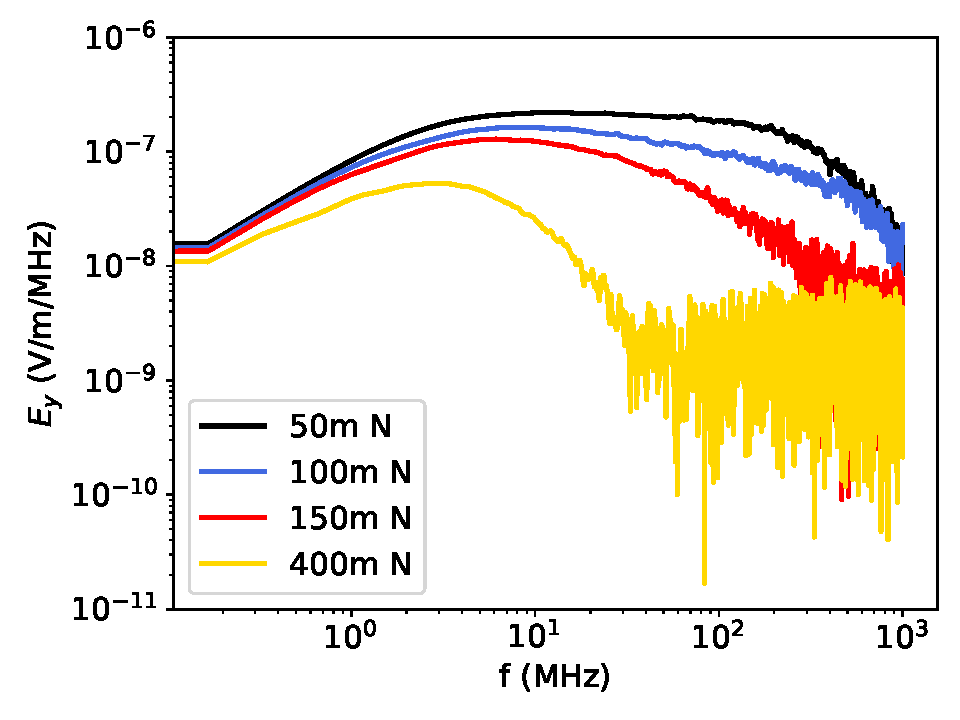
\includegraphics[width=0.45\linewidth]{figures/radio/p_1e17_0deg_EW_N_Fourier_v2}}
	\subfigure[Componente $x$ del campo, al Norte de la cascada.]{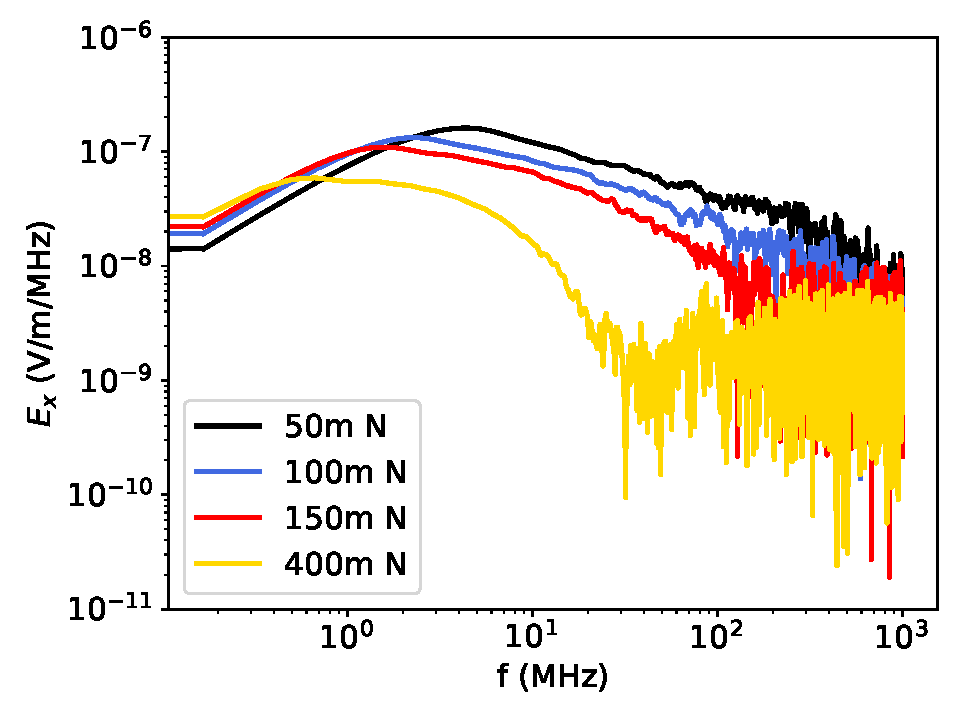
\includegraphics[width=0.45\linewidth]{figures/radio/p_1e17_0deg_NS_N_Fourier_v2}}
	\caption{Transformada de Fourier de las señales en tiempo.}
	\label{E_fields_FFT}
\end{figure}
\begin{figure}[H]
	\centering
	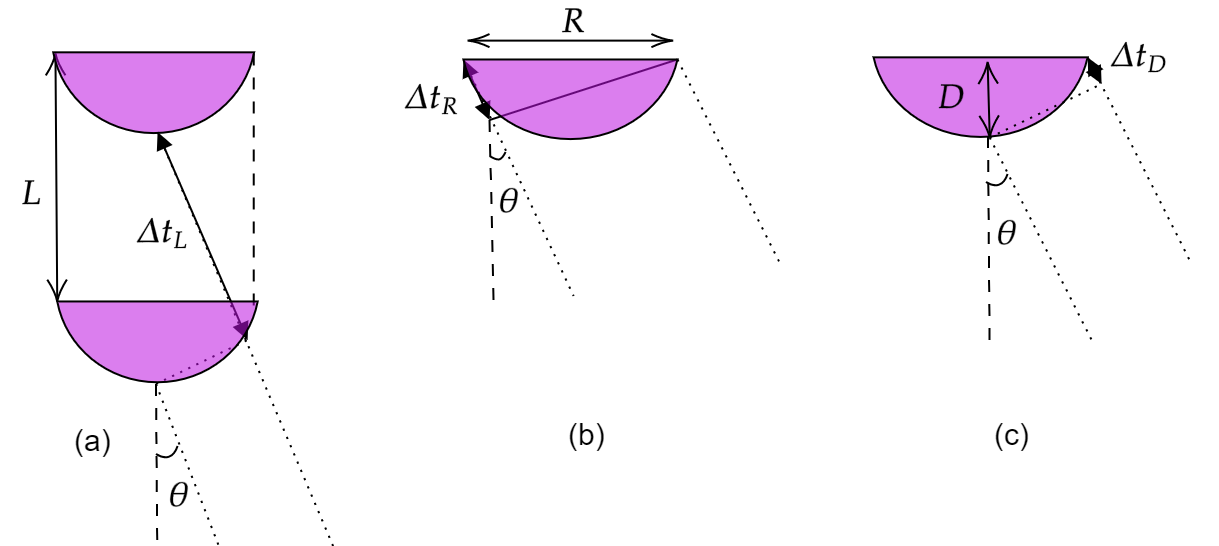
\includegraphics[width=.7\linewidth]{figures/radio/coherence_v2}
	\caption{Modelo geométrico sencillo. (a), (b) y (c) representan las contribuciones respectivas del desarrollo longitudinal, lateral y de \textit{grosor} del frente a los retardos en la señal.}
	\label{coherence}
\end{figure}

Por lo tanto, las emisiones serán coherentes a frecuencias $f\lesssim\Delta t_{max}^{-1}$ (i.e., $\lambda\gtrsim c\Delta t_{max}$, longitudes de onda comparables a las dimensiones de la cascada), donde el máximo de los tres retardos determina el límite a la coherencia. En el caso concreto de cascadas en aire, puede comprobarse\footnote{El modelo geométrico anterior permite hallar fácilmente $\Delta t_{L}=\frac{n}{c}L\cos{\theta}$, $\Delta t_{R}=\frac{n}{c}R\sin{\theta}$. $\Delta t_D$ depende de la forma del frente. Valores típicos en cascadas atmosféricas: $L\sim 5-10\,\mathrm{km}$, $R\sim100\,\mathrm{m}$, $D\sim6\,\mathrm{m}$, $\theta\sim\theta_c\sim1^\circ$, $n\sim1,0003$} que el retardo máximo corresponde a la contribución del \textit{grosor} del frente, $\Delta t_D\sim 20\,\mathrm{ns}$. Por ello, las frecuencias de interés en cascadas atmosféricas se sitúan en el orden de $f\sim\left(20\,\mathrm{ns}\right)^{-1}\sim50\,\mathrm{MHz}$. Aunque el anterior es un modelo muy simple, será suficiente para obtener una intuición del origen de la emisión en radiofrecuencias.

El siguiente caso que plantearemos es el de una cascada inclinada, iniciada por una partícula primaria de mayor energía. Concretamente, se ha simulado una cascada iniciada por un protón de energía $E=10^{19}\,\mathrm{eV}$, con una trayectoria de ángulo cenital $\theta=70^{\circ}$. En este caso, se ha supuesto un campo magnético ligeramente diferente\footnote{ Concretamente, este campo magnético es similar al que se encuentra en el Polo Sur, una localización de especial interés experimental para el estudio de la radiación cósmica.}, de magnitud $55\,\mathrm{\mu T}$ y ángulo de inclinación $I = 72,42^\circ$; mientras que las antenas se han situado a lo largo de las direcciones NS y EW (Fig. \ref{ANITApaper_showscheme}). Esta configuración nos permitirá estudiar algo más en detalle el campo eléctrico observado en función de la posición respecto a la cascada.

Como mencionamos en el primer apartado de esta sección, el máximo de la emisión ocurre cuando el ángulo de observación coincide con el ángulo \v{C}erenkov. Además, hemos visto en la sección \ref{sec2} cómo el desarrollo de cascadas atmosféricas presenta, a cierta profundidad en la atmósfera que depende de los parámetros del primario, un máximo claro del número de partículas. Por ello, en el suelo se registrará el máximo del campo eléctrico en las antenas que observen dicho máximo de la cascada bajo un ángulo $\theta_C$, i.e, en la intersección del suelo con el cono \v{C}erenkov. 
\begin{figure}[H]
	\centering
	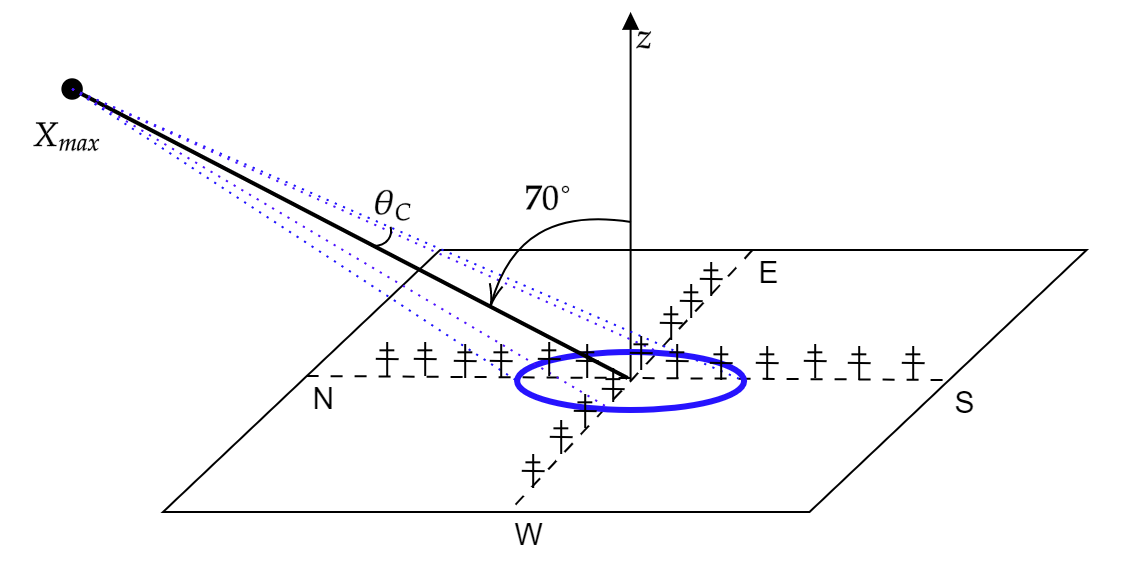
\includegraphics[width=.65\linewidth]{figures/radio/ANITApaper_showscheme}
	\caption{Configuración planteada. Se situaron 50 antenas a lo largo de cada eje, hasta $1500\,\mathrm{m}$ del \textit{core} de la cascada. El máximo de emisión se espera en la intersección del cono \v{C}erenkov., cuyo vértice se sitúa en el máximo del desarrollo.}
	\label{ANITApaper_showscheme}
\end{figure}

Evidentemente, para una cascada inclinada la intersección del cono \v{C}erenkov con el suelo no será una circunferencia sino una elipse. Si para esta configuración representamos el máximo de la componente EW del campo eléctrico registrado en cada antena, obtenemos la Fig. \ref{downgoing_p_10EeV_70deg_Ey_t_ground}. El resultado no es especialmente esclarecedor, ya que esperaríamos dos máximos bien definidos a lo largo de los dos ejes. Si bien puede intuirse un comportamiento así en las antenas situadas a lo largo de la dirección NS, no ocurre así para la dirección EW.

Lo que haremos será estudiar el campo eléctrico en el dominio de frecuencias, en lugar de representar el máximo en tiempo como hemos hecho. Presentamos en la Fig. \ref{freqfieldsgrounds} algunas componentes de Fourier obtenidas con la configuración de la Fig. \ref{ANITApaper_showscheme}. En este caso sí aparecen perfectamente definidos los máximos asociados al cono \v{C}erenkov, estando más separados en la dirección N-S como era de esperar, dada la inclinación de la cascada.

\clearpage
\begin{figure}[H]
	\centering
	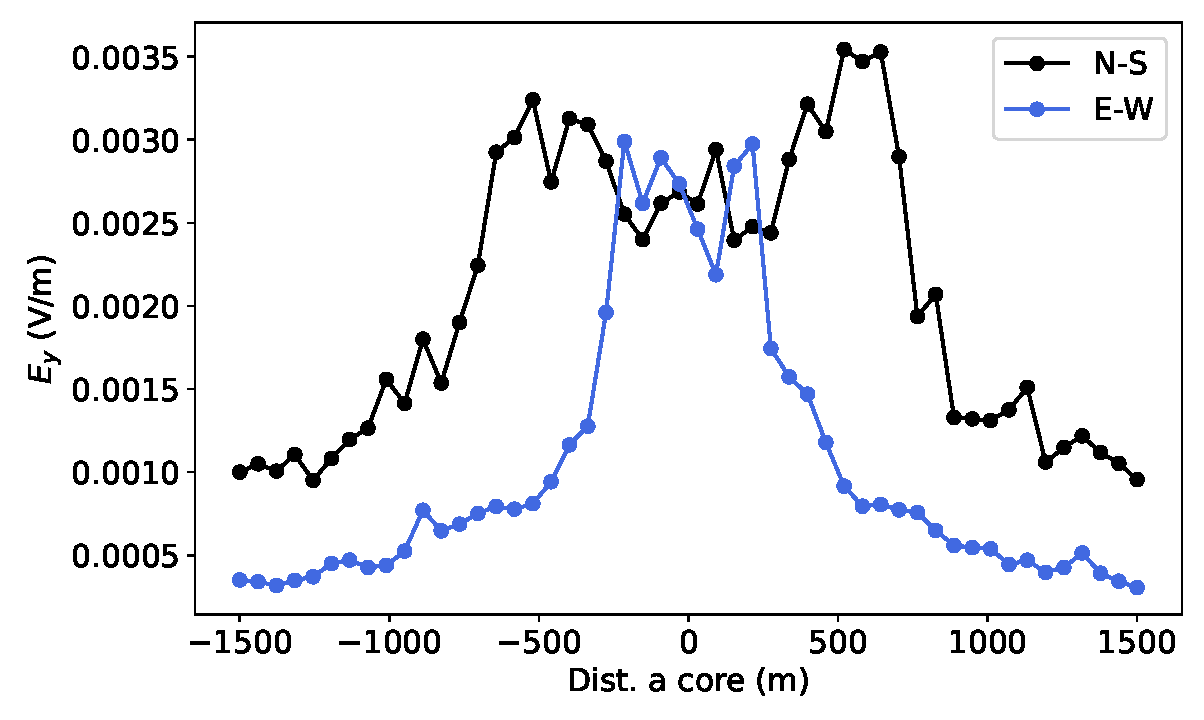
\includegraphics[width=.65\linewidth]{figures/radio/downgoing_p_10EeV_70deg_Ey_t_ground_v2}
	\caption{Máximo del campo eléctrico registrado en las antenas a nivel del suelo de la configuración \ref{ANITApaper_showscheme}. Se representan los valores en los dos ejes (NS, EW).}
	\label{downgoing_p_10EeV_70deg_Ey_t_ground}
\end{figure}

\begin{figure}[H]
	\centering
	\subfigure[Componente $y$ del campo a $300\,\mathrm{MHz}$]{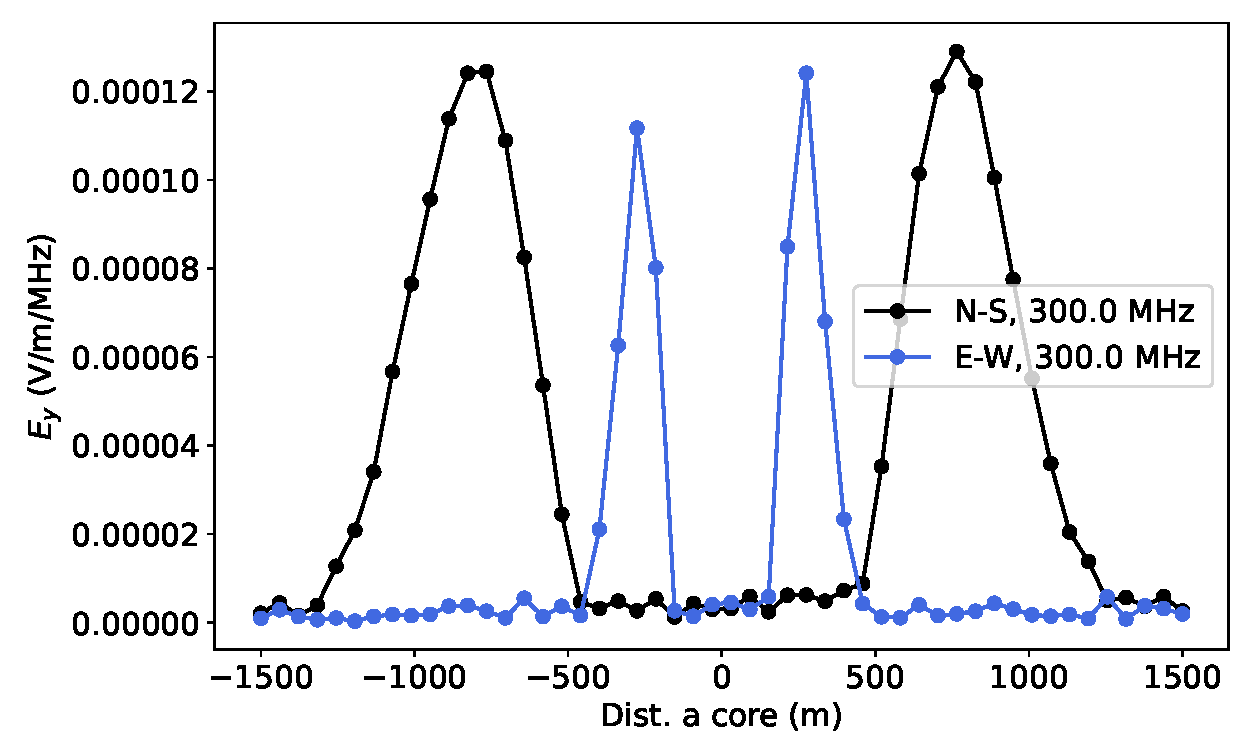
\includegraphics[width=0.49\linewidth]{figures/radio/downgoing_p_10EeV_70deg_Ey_300MHz_ground_v2}}
	\subfigure[Componentes a varias frecuencias a lo largo de la dirección EW]{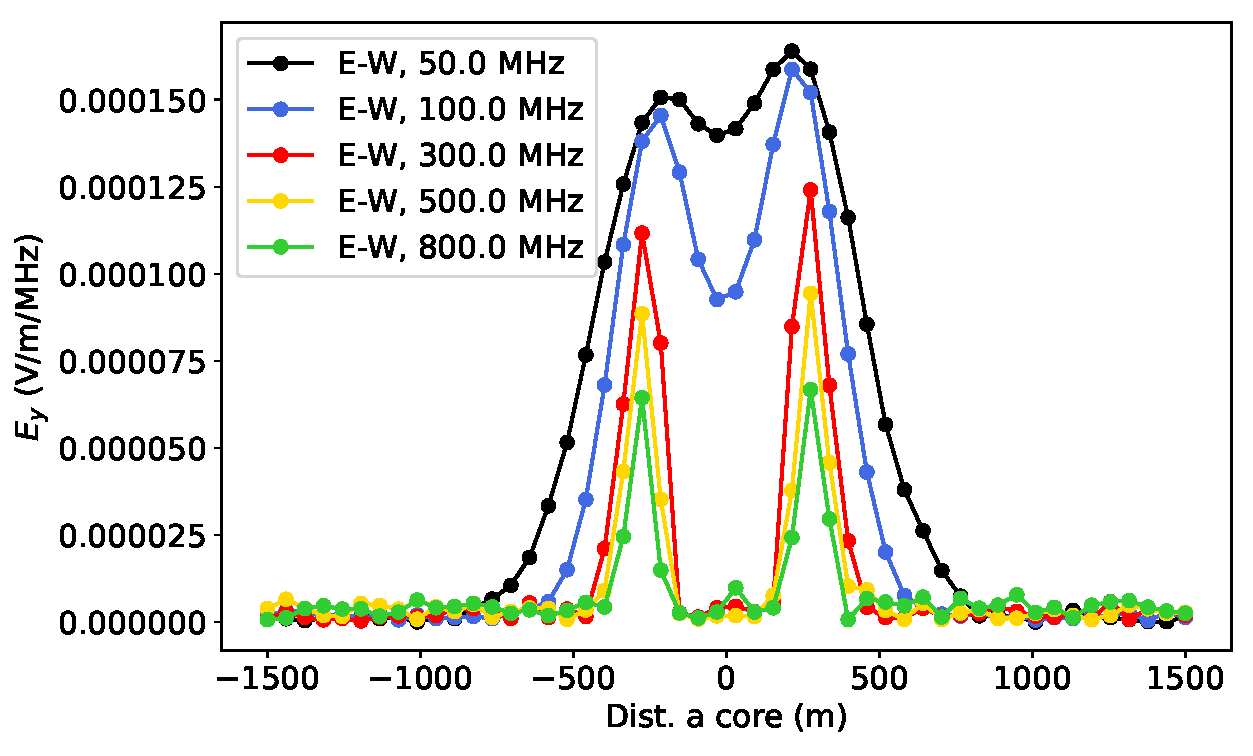
\includegraphics[width=0.49\linewidth]{figures/radio/downgoing_p_10EeV_70deg_Ey_varfreq_groundEW_v2}}
	\caption{Componentes de Fourier del campo eléctrico (componente $y$) en función de la distancia al \textit{core} de la cascada.}
	\label{freqfieldsgrounds}
\end{figure} 


%Como ya mencionamos, ZHAireS permite obtener el espectro en frecuencia del campo eléctrico en cada antena. Antes de presentar los resultados que hemos obtenido de esta manera, haremos una breve digresión acerca de los valores de frecuencia que debemos considerar.

%La estimación más rápida para las frecuencias asociada a la radiación electromagnética emitida puede hacerse a partir de los resultados \ref{EW_field} y \ref{NS_field}. Puesto que tiempo y frecuencia son variables conjugadas de Fourier, la duración de los pulsos nos da un orden de magnitud para $f$:
%\begin{equation}
%	\omega T = 2\pi f T \sim 1\implies f\sim \left(2\pi T\right)^{-1} \implies T \sim 1 \,\mathrm{ns} \leftrightarrow f \sim 100 \,\mathrm{MHz}\label{ec317}
%\end{equation} 
%Por lo tanto, podemos adelantar que las frecuencias de interés estarán en el rango de las radiofrecuencias ($\sim30\,\mathrm{MHz}-1\,\mathrm{GHz}$). Una razón para que la emisión relevante aparezca en esta banda de frecuencias puede verse con argumentos sencillos de coherencia, i.e., exigiendo que la longitud de onda sea comparable a las dimensiones de la cascada:
%	\begin{figure}[H]
%		\centering
%		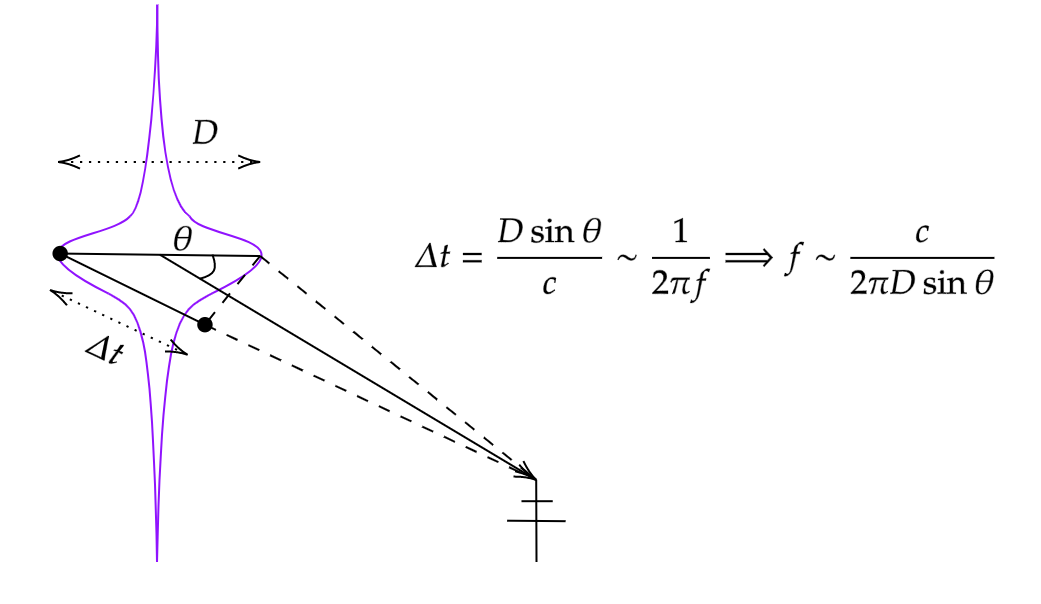
\includegraphics[width=.6\linewidth]{figures/radio/coherence}
%		\caption{Geometría considerada. $D$ se corresponde con el desarrollo lateral de la cascada en el máximo.}
%		\label{coherence}
%	\end{figure}
%Tomando valores típicos para una cascada en la atmósfera ($D\sim 100\,\mathrm{m}$, $\theta\sim\theta_C\sim1^\circ$), se encuentra $f\sim30\,\mathrm{MHz}$. Por lo tanto, debemos quedarnos con que los rangos de frecuencia que nos interesan son de radiofrecuencias.

 La explicación para los resultados de la Fig. \ref{downgoing_p_10EeV_70deg_Ey_t_ground} puede extraerse de la gráfica de la derecha, en la que representamos las componentes de Fourier del campo a varias frecuencias. Como vemos la amplitud de las componentes decrece al aumentar la frecuencia\footnote{ Tomando el límite $\theta\rightarrow\theta_C$ de manera adecuada en \eqref{ec316} puede verse que $\vect{E}\left(\vect{r},\omega\right)\propto\omega$.}, aunque quizá el efecto más relevante es que la \textit{resolución} de los máximos disminuye cuanto menor sea $f$, llegando a estar prácticamente superpuestos para las frecuencias más bajas. 

La explicación a este hecho puede encontrarse en fenómenos de tipo difractivo. Podemos ejemplificarlo recordando, e.g., el patrón de Airy, en el que el primer cero del patrón de difracción ocurre cuando, respecto al máximo, observamos bajo un ángulo $\alpha$ tal que:
\begin{equation}
	\sin\alpha=1,22\frac{\lambda}{d}\label{ec318}
\end{equation}  
donde $d$ es el tamaño típico de la fuente. Evidentemente, a menor (mayor) frecuencia (longitud de onda), debemos irnos hasta un mayor $\alpha$ para encontrar el mínimo del patrón. Es decir, cuanto menor sea la frecuencia mayor será la anchura del pico, como observamos en \ref{freqfieldsgrounds}b

Evidentemente, en la Fig. \ref{downgoing_p_10EeV_70deg_Ey_t_ground} estábamos viendo la superposición de todas las componentes de Fourier, y debido a que las dominantes (menores frecuencias) no están resueltas, no se observaba claramente la intersección del cono \v{C}erenkov con el suelo.

Para acabar esta sección, recapitularemos los resultados y conclusiones más importantes:
\begin{enumerate}
	\item En cascadas atmosféricas tendremos dos contribuciones fundamentales a la emisión de radiación electromagnética: deflexión geomagnética y efecto Askaryan, cada una con efectos diferentes en la polarización del campo detectado.
	\item Las expresiones deducidas para el campo eléctrico radiado no asumen ningún mecanismo de emisión, y están integradas en el código ZHAireS empleado para realizar las simulaciones. Como hemos visto, el efecto de ambos mecanismos es evidente en los resultados.
	\item Las frecuencias de interés se sitúan en la banda de los $\mathrm{MHz}$ (radiofrecuencias). Además, la señal de campo eléctrico detectada tiene una dependencia importante con la frecuencia, tanto en amplitud (mayor a menores frecuencias) como en la resolución de los máximos en torno al ángulo \v{C}erenkov.
\end{enumerate}
\clearpage

	\section{Emisión en radio en cascadas hacia arriba}
	Partiendo de los desarrollos y resultados que hemos presentado en secciones anteriores, podemos pasar al objetivo final de este trabajo: la descripción y caracterización de la emisión en radiofrecuencias producida por cascadas atmosféricas \textit{hacia arriba}. Concretamente, nos interesará describir mediante simulaciones la radiación asociada a cascadas muy inclinadas iniciadas por la desintegración de un leptón $\tau$, originado a partir de un neutrino tau de origen astrofísico.  
	
	Antes de pasar a discutir la emisión en dichos eventos, podemos servirnos de desarrollos previos para, en cierto modo, adelantar el comportamiento que esperamos, algo que nos permitirá llegar a una interpretación clara de nuestros resultados. En primer lugar, hemos visto en la sección \ref{sec3} que los picos de emisión se sitúan en las posiciones que observan el máximo del desarrollo bajo el ángulo \v{C}erenkov. En cascadas hacia arriba ocurrirá exactamente lo mismo, salvo que (evidentemente) las dimensiones del \textit{anillo} \v{C}erenkov aumentarán con la altura en la atmósfera. Un ejemplo de este comportamiento se presenta en la Fig. \ref{Comparativa_20_36km}, en la que presentamos varias componentes de campo eléctrico obtenidas en simulaciones con ZHAireS de una cascada vertical hacia arriba. Aunque la observación de un evento similar es altamente improbable, muestra claramente el comportamiento esperado.
	\begin{figure}[H]
		\centering
		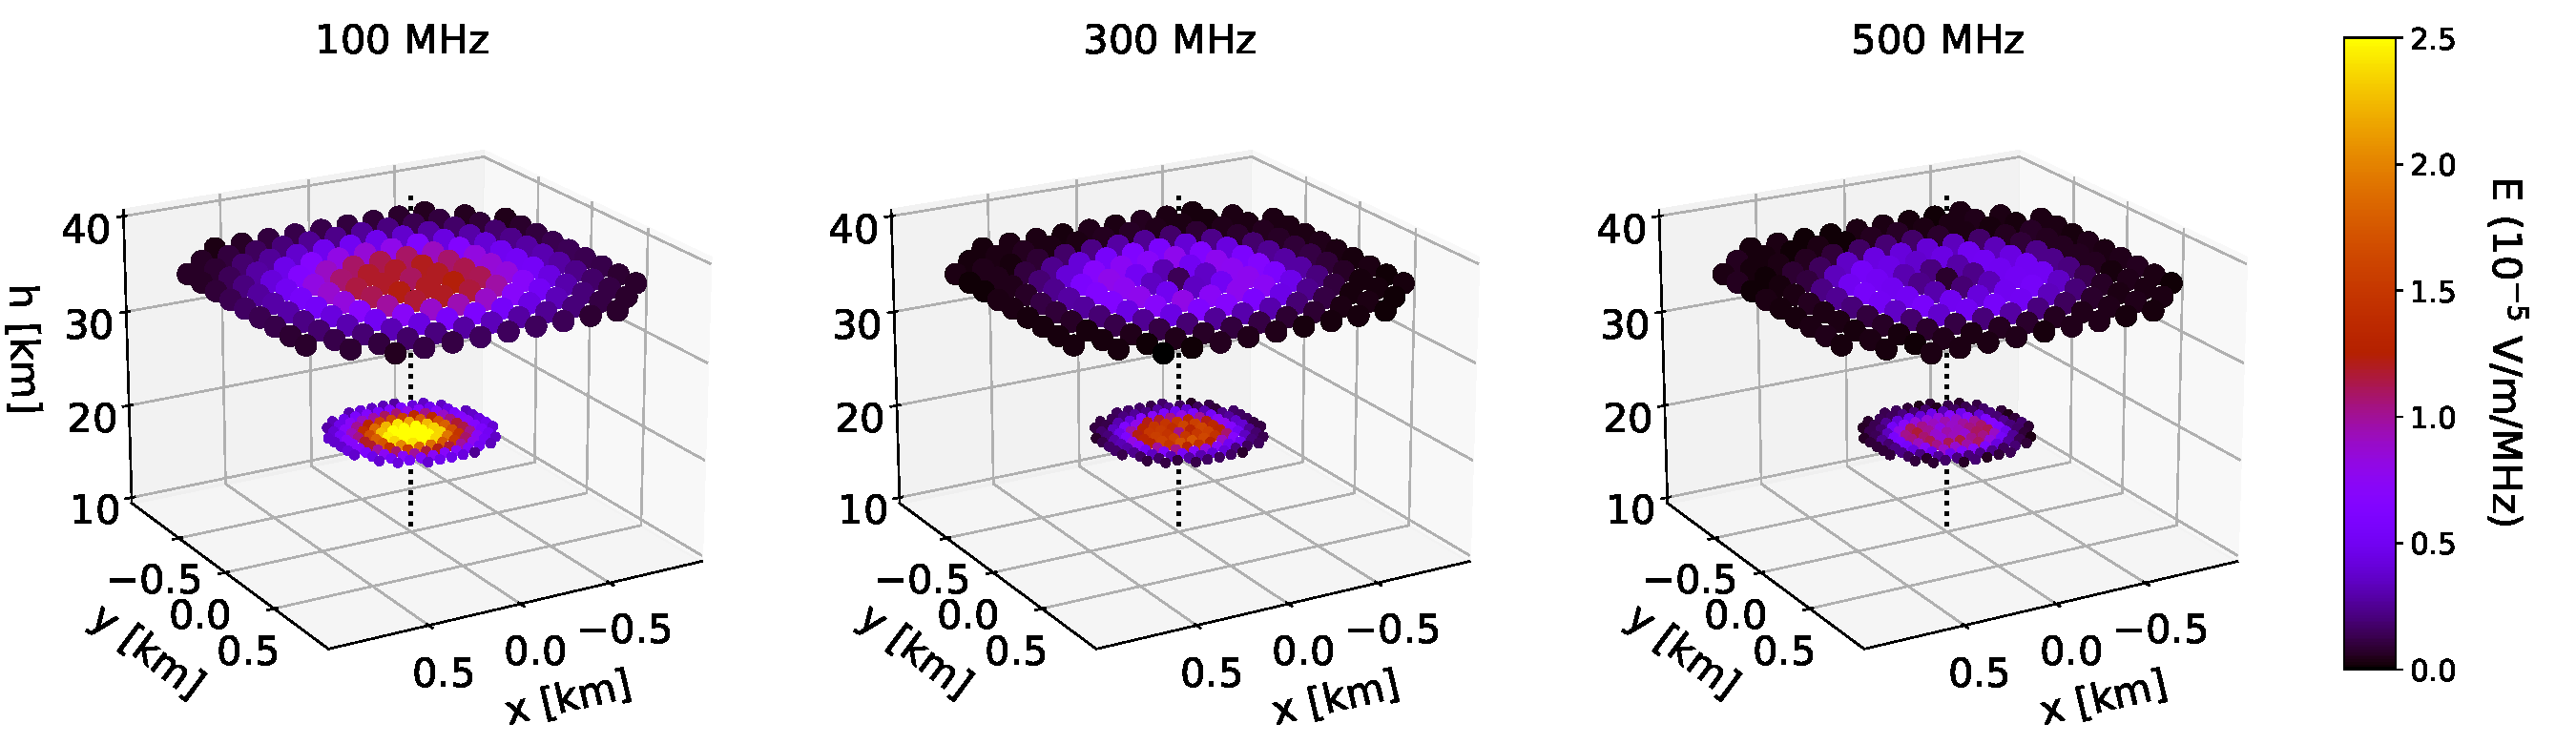
\includegraphics[width=1.\linewidth]{figures/Radio_UG/Comparativa_20_36km}
		\caption{Componentes de Fourier del campo eléctrico generado por una cascada vertical hacia arriba ($\theta=180^\circ$) iniciada por un protón de $1\,\mathrm{EeV}$ interaccionando a nivel del suelo, observadas a $20$ y $36\,\mathrm{km}$ de altura. La línea punteada señala el eje de la cascada.}
		\label{Comparativa_20_36km}
	\end{figure}
De la misma manera que en el caso discutido en la sec. \ref{sec32}, la inclinación del eje de la cascada hará que, a cada altura, los máximos de la emisión se dispongan en una elipse, de nuevo asociada al cono \v{C}erenkov. No obstante, existirá una ligera diferencia respecto al caso de las cascadas hacia abajo. Para mostrarla claramente, presentamos en la Fig. \ref{Comparativa_0_45deg} el resultado de simulaciones de ZHAireS para una cascada iniciada por protón a $0\,\mathrm{km}$ de altura, con el eje en la dirección vertical o inclinado a $45^\circ$ (\textit{hacia arriba}, $\theta=135^\circ$). Para la cascada inclinada, apreciamos claramente que el campo eléctrico observado es más intenso al oeste del eje de la cascada ($y>0$), justo al contrario de lo que ocurría en cascadas hacia abajo (Fig. \ref{EW_field}). La razón para este comportamiento es simplemente el hecho de que, en este caso, el nivel de observación se sitúa por encima del máximo de la cascada, que además se desarrolla en el sentido opuesto. Debido a este cambio, las contribuciones de la deflexión geomagnética y efecto Askaryan se añadirán en posiciones al oeste en lugar de al este. En la Fig. \ref{Polarizacion_UG} presentamos un esquema similar a las Figs. \ref{Geomag_deflexion}, \ref{Askaryan} aplicado a este caso.
	\begin{figure}[H]
	\centering
	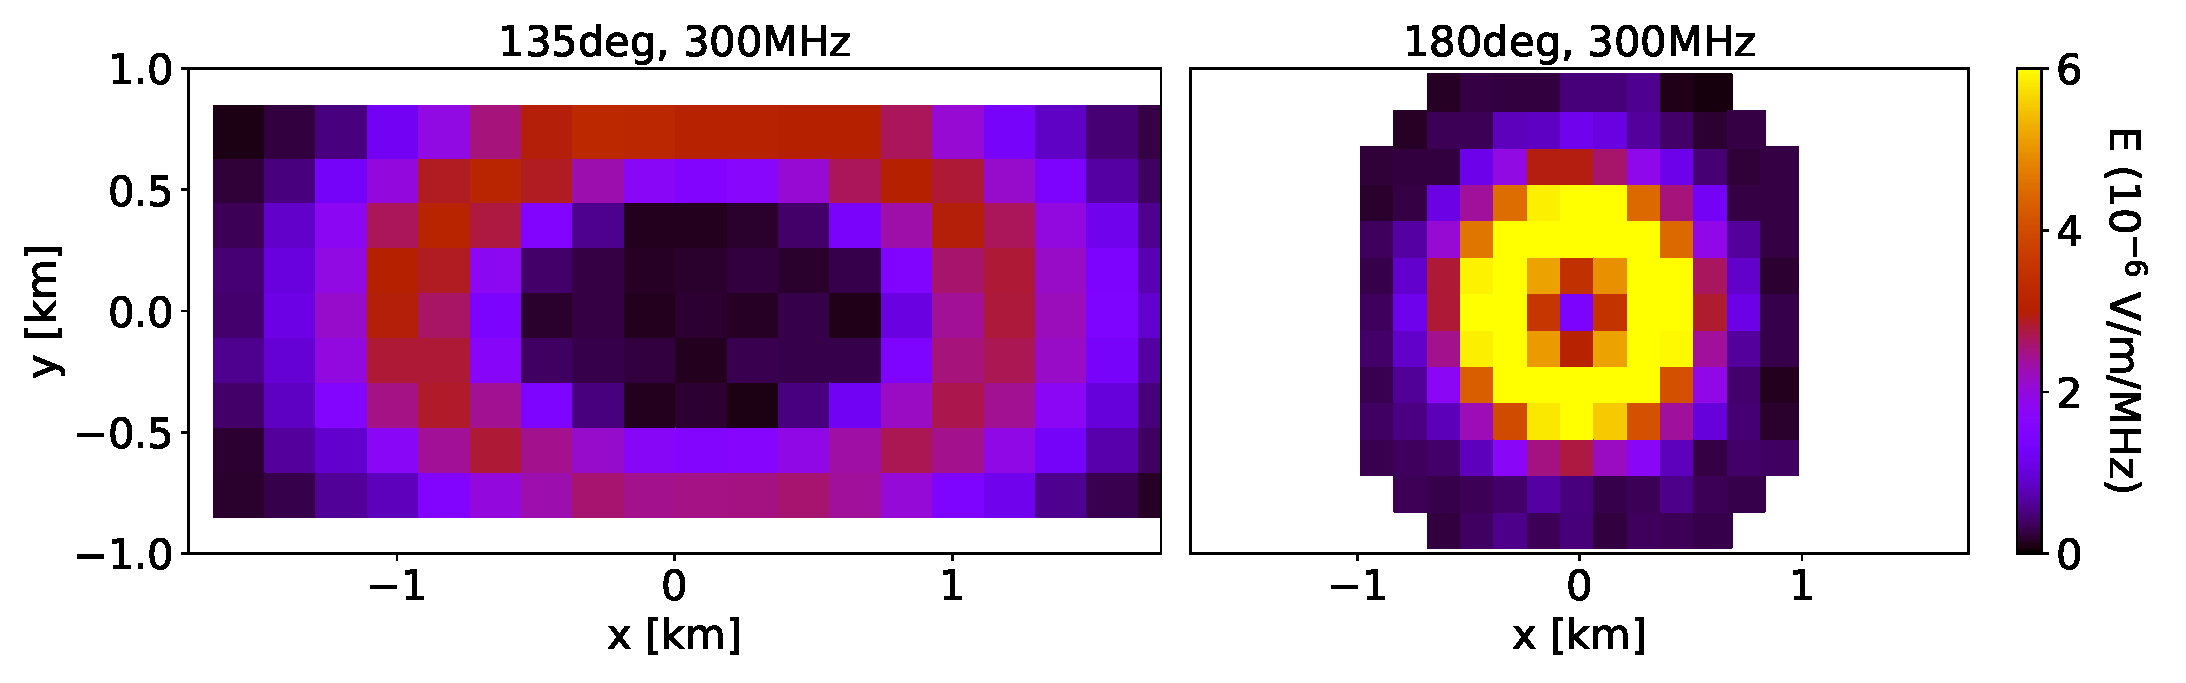
\includegraphics[width=.8\linewidth]{figures/Radio_UG/Comparativa_0_45deg}
	\caption{Componente a $300\,\mathrm{MHz}$ del campo eléctrico generado por una cascada inclinada (vertical) hacia arriba iniciada por un protón de $1\,\mathrm{EeV}$ interaccionando a nivel del suelo, observada a $36\,\mathrm{km}$ de altura.}
	\label{Comparativa_0_45deg}
\end{figure}


\begin{figure}[H]
	\centering
	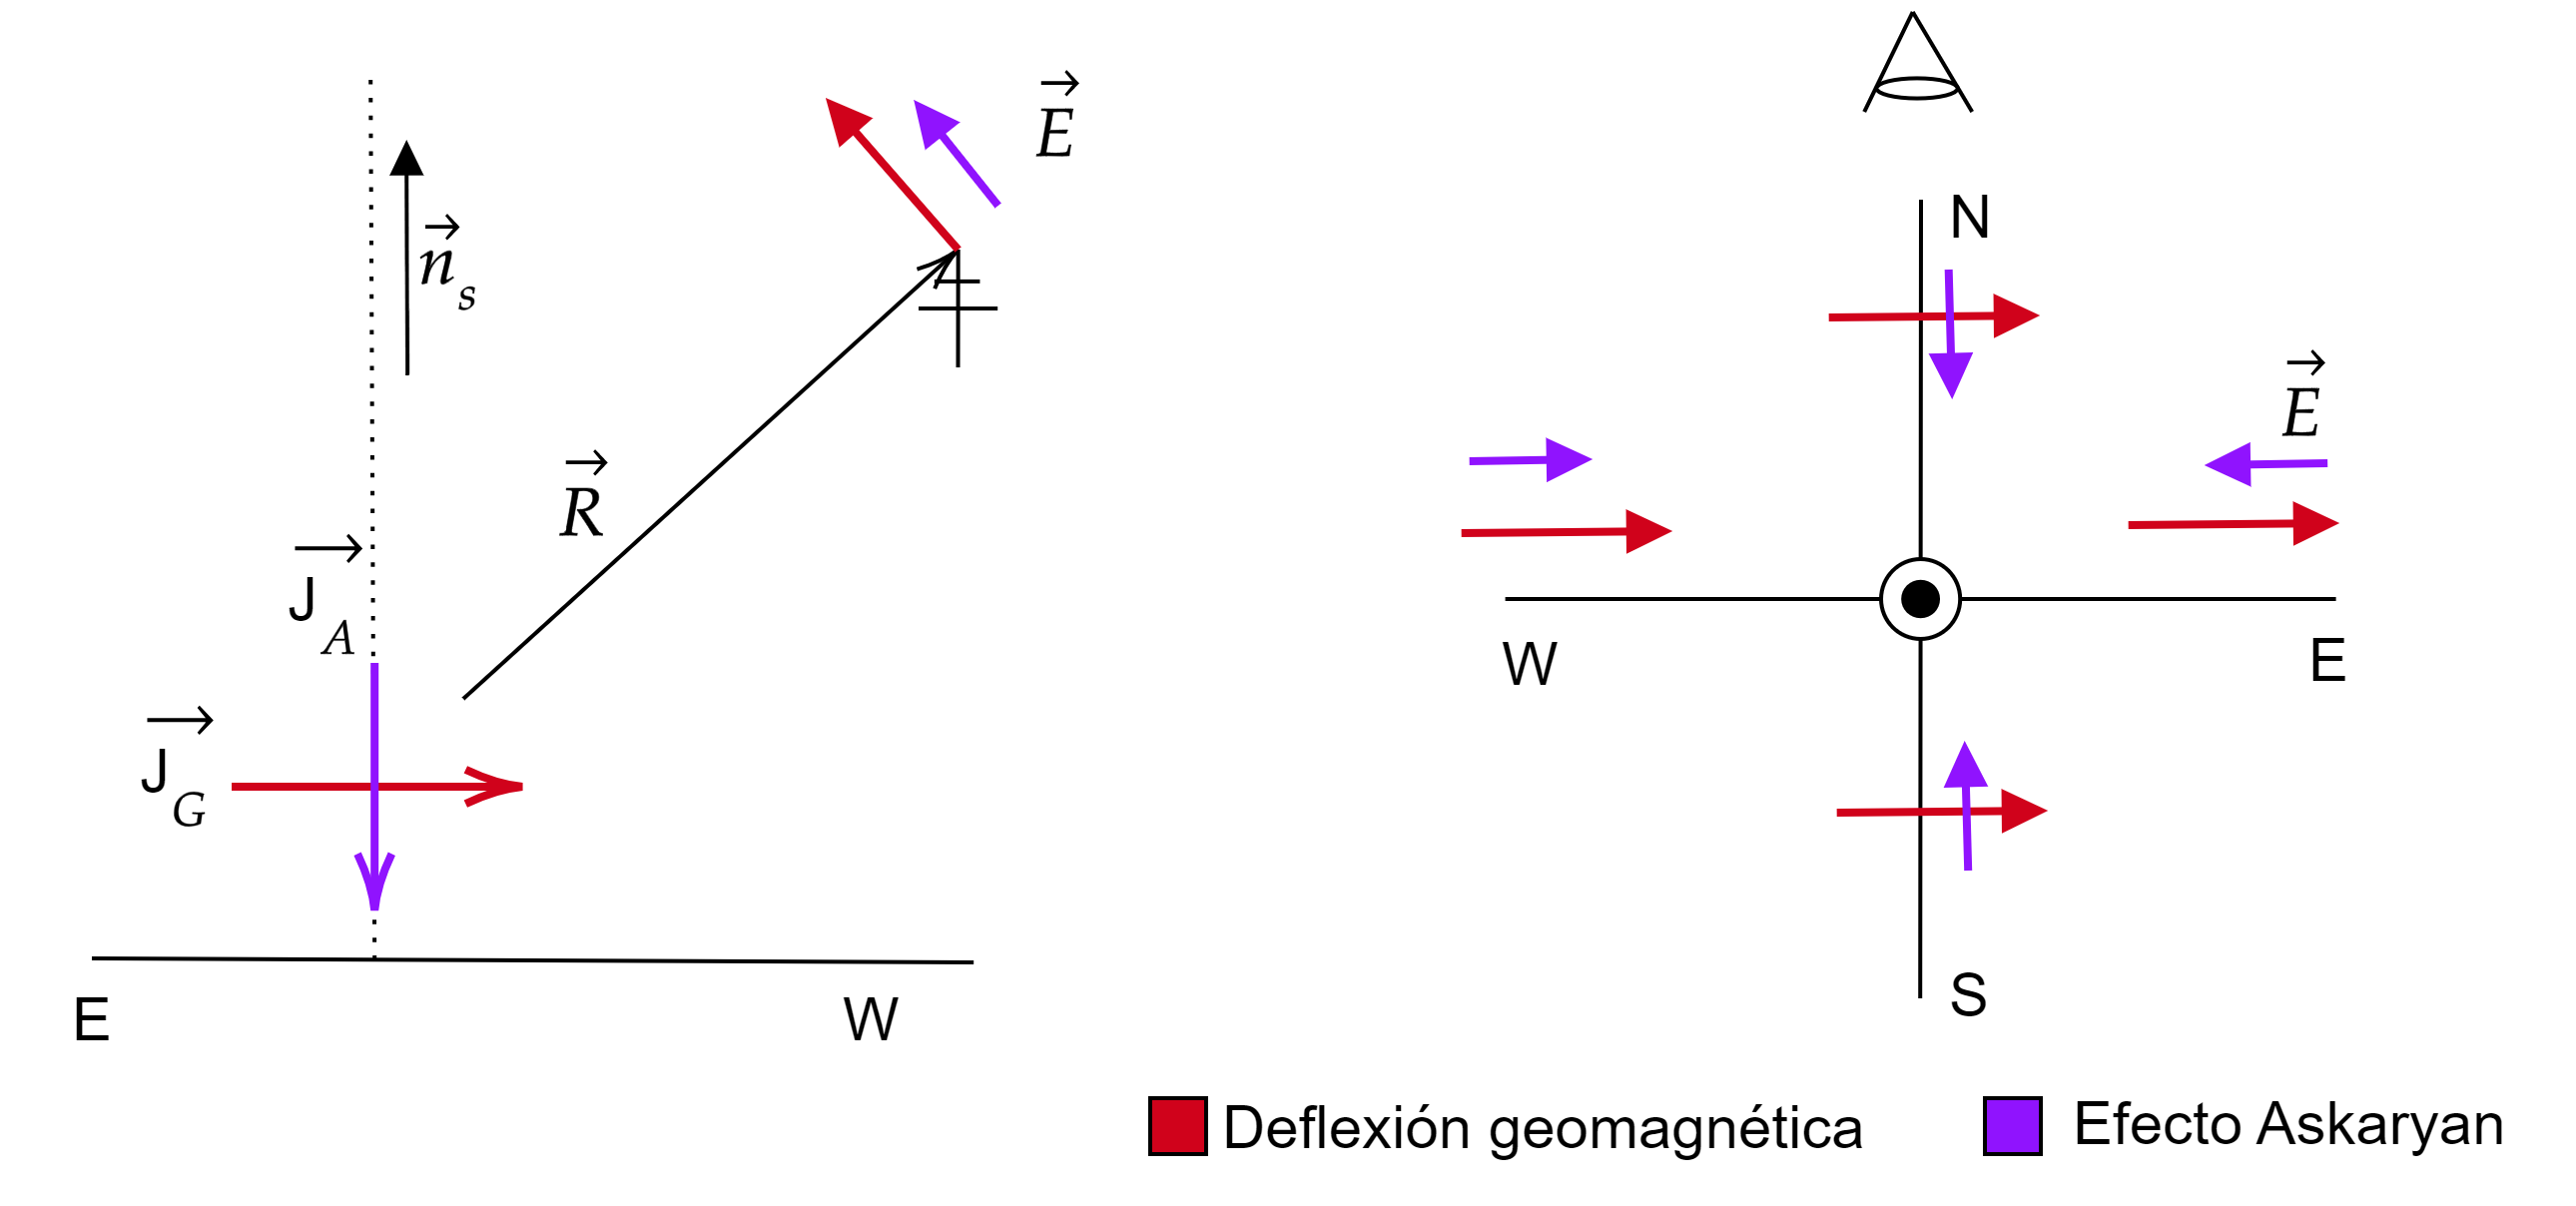
\includegraphics[width=.7\linewidth]{figures/Radio_UG/Polarizacion_UG}
	\caption{Contribuciones a la radiación electromagnética observada por encima del máximo en cascadas hacia arriba.}
	\label{Polarizacion_UG}
\end{figure}
Por todo lo anterior, esperaremos que la emisión en radio asociada a cascadas atmosféricas muy inclinadas y hacia arriba esté marcada por la presencia de una \textit{elipse} \v{C}erenkov cuyas dimensiones aumentarán con la altura de observación. Además, las dos contribuciones fundamentales a la emisión son tales que el campo eléctrico observado será superior en posiciones al oeste del eje de la cascada.

Con esta breve discusión previa, podemos pasar a estudiar un caso más realista y de mayor interés. Para caracterizar la emisión de radiación en los eventos asociados a las desintegraciones de leptones $\tau$, hemos partido de las siguientes consideraciones:

\begin{itemize}
	\item El leptón $\tau$ posee numerosos modos de desintegración. Su elevada masa ($\sim 1,8\,\mathrm{GeV}$) permite que, en más de un $60\%$ de las ocasiones, la desintegración sea hadrónica ($\tau^-\rightarrow\text{Had}+\nu_\tau$). En menor proporción la desintegración puede ocurrir a leptones ($\tau^-\rightarrow e^-\bar{\nu}_e\nu_\tau$, $\tau^-\rightarrow \mu^-\bar{\nu}_\mu\nu_\tau$ y sus conjugados). Como vimos en la sec. \ref{sec22}, la naturaleza leptónica o hadrónica de las partículas que inician la cascada no introduce una dependencia fuerte en el número máximo de partículas producidas en el desarrollo. Por ello, y por simplicidad en las simulaciones\footnote{ AIRES no considera leptones $\tau$ en las simulaciones (v. 2.6)}, partiremos de protones como partículas primarias interaccionando a $0\,\mathrm{km}$ de altura. Esta aproximación no restará realismo a los resultados, además de que las cascadas con componente hadrónica serán las más frecuentes en esta clase de eventos dadas las desintegraciones del $\tau$.
	
	\item En cascadas muy inclinadas hacia arriba e iniciadas a $0\,\mathrm{km}$ de altura, el máximo del desarrollo se alcanza rápidamente, en las proximidades del nivel del suelo (resultados discutidos en la sec. \ref{sec22}). Estudiaremos el caso de cascadas hacia arriba con $\theta=95^\circ$ en las que la posición del máximo encontrada en las simulaciones fue:
	\begin{equation}
		X_{v}^{max}=965\,\mathrm{g/cm^2}\label{ec51}
	\end{equation} 
Para un ángulo de $95^\circ$, el máximo del desarrollo (i.e., el vértice del cono \v{C}erenkov) se alcanzaría a una altura de aproximadamente $600\,\mathrm{m}$ sobre el nivel del suelo, muy por debajo de las alturas de observación que consideraremos.
\end{itemize}

Resumiendo, simularemos la emisión en radio en cascadas atmosféricas a $\theta=95^\circ$ iniciadas por protones interaccionando a $0\,\mathrm{km}$ de altura. Por simplicidad, hemos tomado en todas las simulaciones un campo magnético terrestre totalmente paralelo al suelo y de intensidad $50\,\mathrm{\mu T}$, y hemos escogido una dirección de desarrollo hacia el norte magnético (i.e., azimut $\phi=0$). Además, trabajaremos en el dominio de frecuencias para poder obtener resultados claros en los que no haya que considerar la evolución temporal de la señal. 

Naturalmente, el objetivo fundamental de la observación de la radiación emitida en cascadas atmosféricas debe ser la extracción de información sobre la partícula primaria, fundamentalmente acerca de su naturaleza, energía y dirección de llegada. Para estudiar precisamente cómo dicha información estaría contenida en el campo eléctrico observado, hemos realizado simulaciones para tres valores de energía del primario ($10\,\mathrm{PeV}$, $100\,\mathrm{PeV}$, $1\,\mathrm{EeV}$) y situando las alturas de observación a 5, 36 y 100 $\mathrm{km}$ de altura (siendo las dos primeras especialmente adecuadas para los experimentos BEACON y PUEO respectivamente). Los resultados obtenidos para las componentes de Fourier a $100$, $300$ y $500\,\mathrm{MHz}$ del campo eléctrico se presentan en las Figs. \ref{85deg_varh_536100} (variando altura de observación)  y \ref{85deg_varE} (variando la energía del primario).

Como ya habíamos adelantado, lo primero que observamos son los máximos de campo eléctrico distribuidos en la elipse \v{C}erenkov, que debido a la gran inclinación del eje de la cascada alcanza grandes dimensiones, que a su vez aumentan con la altura de observación (desde $\sim30\times5\,\mathrm{km^2}$ a $5\,\mathrm{km}$ de altura hasta $\sim500\times50\,\mathrm{km^2}$ a $100\,\mathrm{km}$). Además, observamos claramente cómo la señal registrada al oeste del eje de la cascada es más intensa, debido precisamente a los mecanismos de deflexión geomagnética y efecto Askaryan contribuyendo de manera \textit{constructiva}. En el caso concreto que hemos simulado, tanto la inclinación como la orientación del eje del desarrollo hacia el norte magnético hacen que la contribución geomagnética (que depende del producto $\hat{\vect{n}}_s\times\vect{B}$) no domine sobre la contribución Askaryan, haciendo que el efecto predicho sea especialmente visible. Además, el \textit{anillo} aparece cada vez mejor definido al aumentar la frecuencia a la que observamos, un fenómeno que ya habíamos encontrado en la caracterización general de la radiación emitida en cascadas (Fig. \ref{freqfieldsgrounds})

En lo que respecta a la extracción de información acerca de la naturaleza del primario, es evidente que la \textit{elipse} \v{C}erenkov y su orientación y dimensiones están claramente relacionadas con la dirección de llegada de la partícula primaria. Por ello, la extracción de esta clase de información podría realizarse observando directamente esta estructura, o una parte de la misma, en un array de antenas de dimensión suficiente. 
\begin{figure}[H]
		\centering
		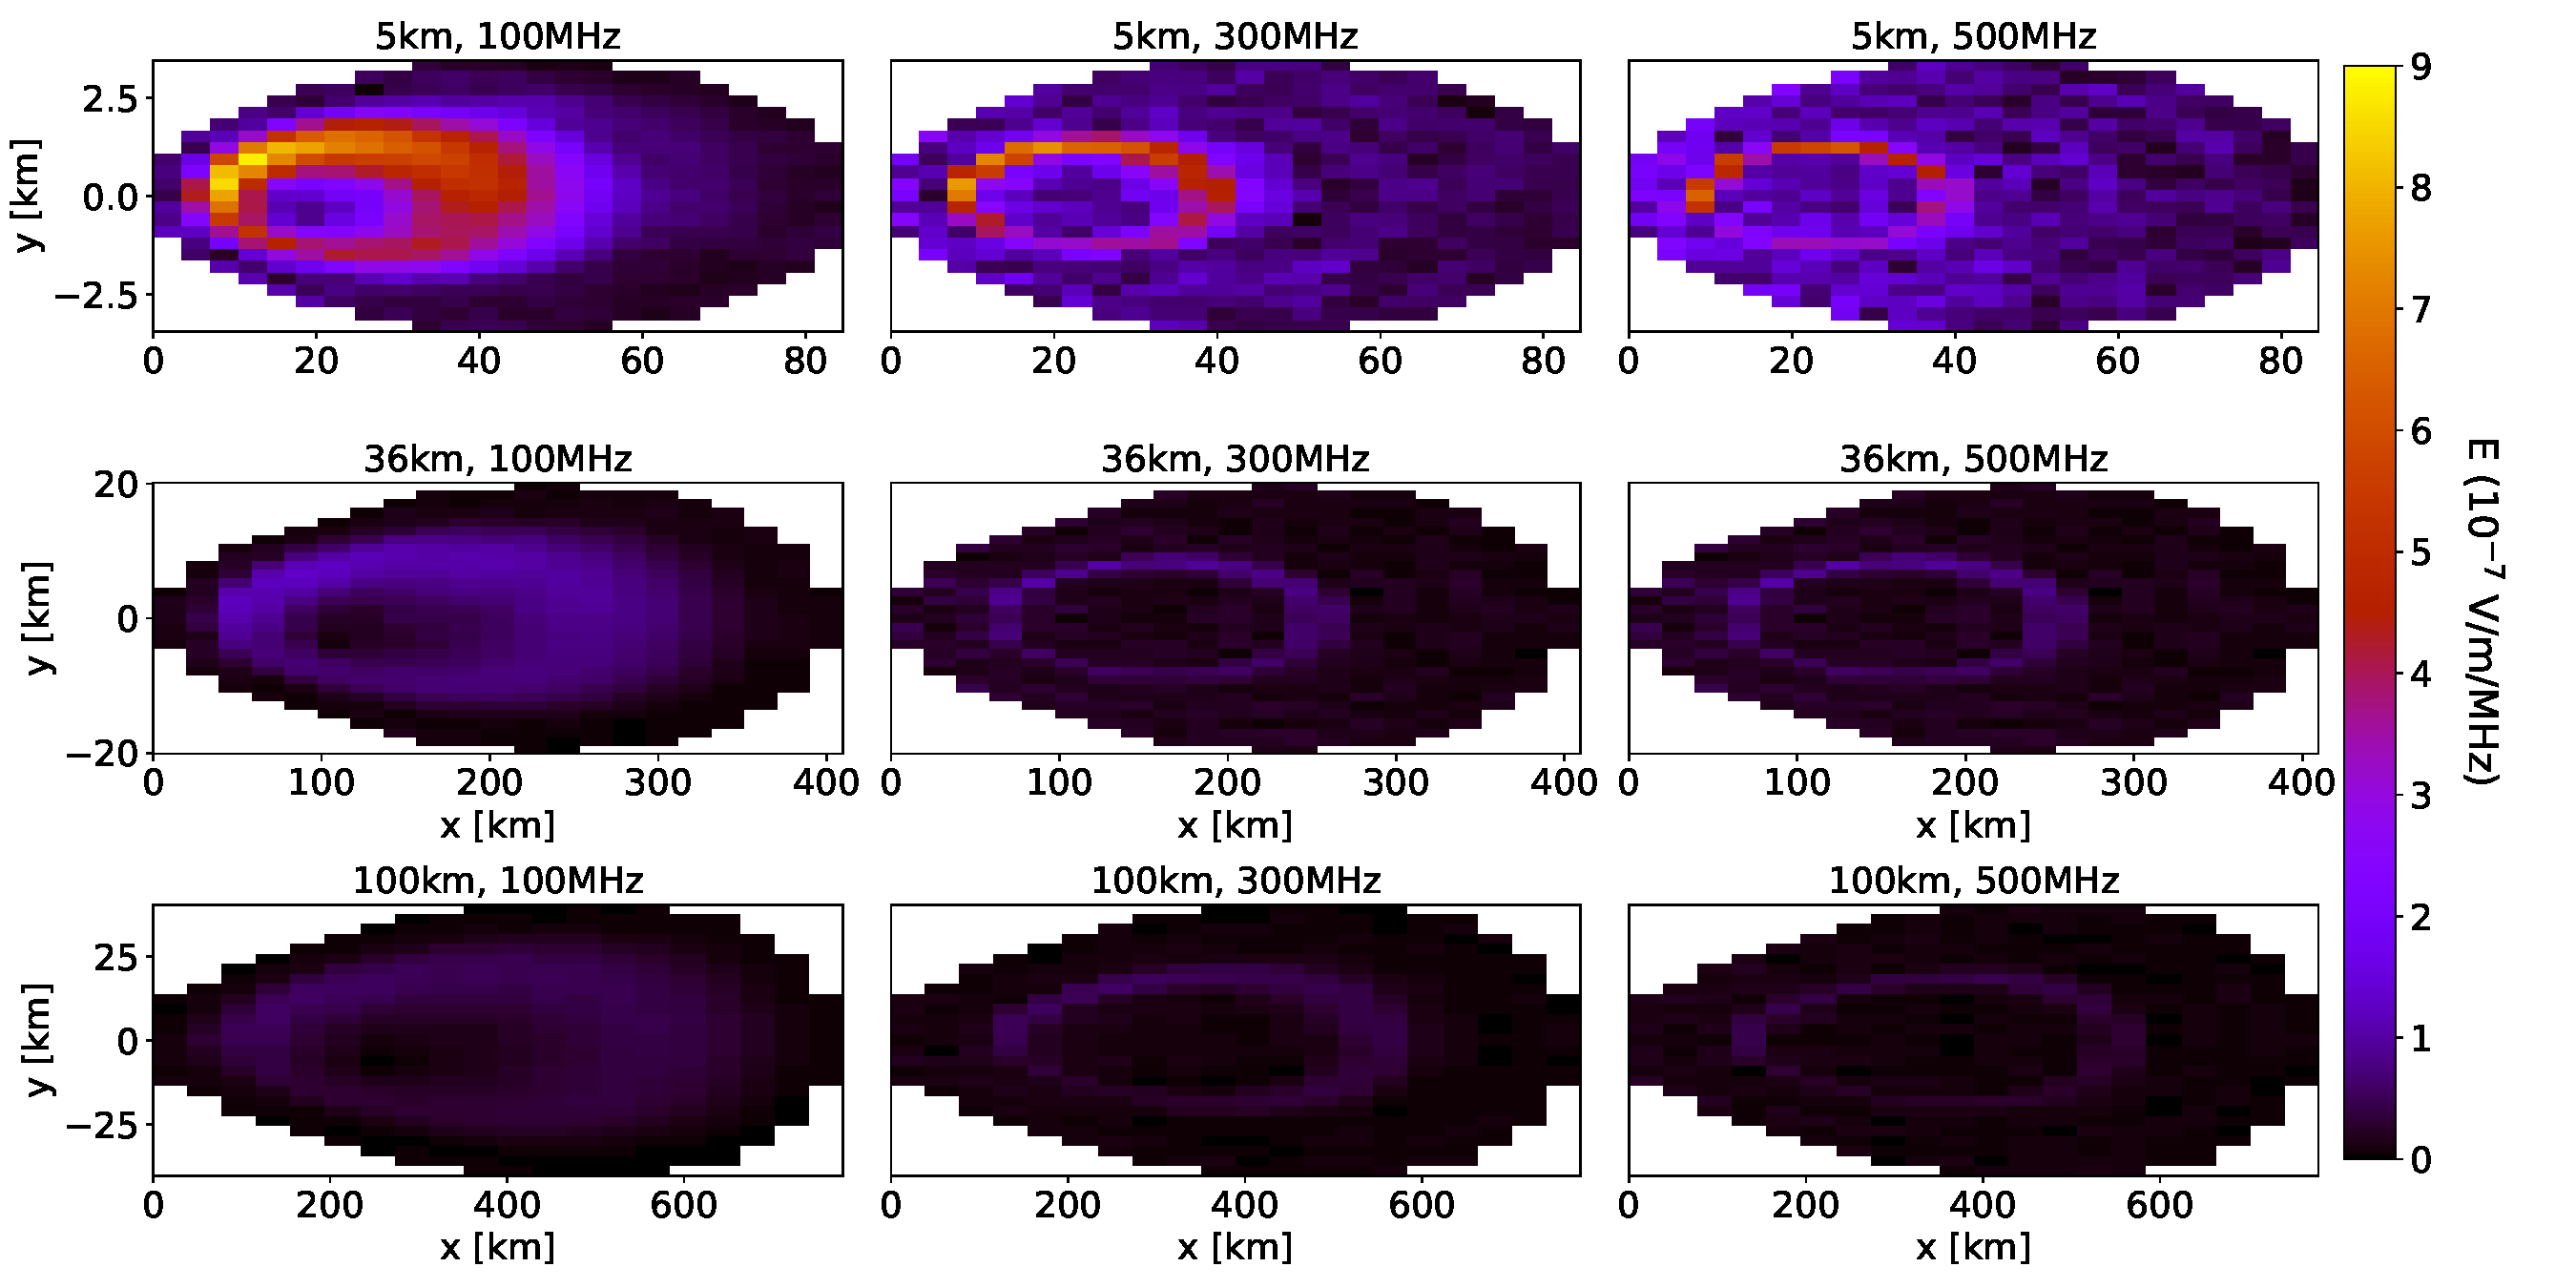
\includegraphics[width=.95\linewidth]{figures/Radio_UG/85deg_varh_5_36_100}
		\caption{Componentes de Fourier del campo eléctrico observado a diversas alturas. El origen de coordenadas $xy$ es arbitrario, se ha escogido para apreciar fácilmente las dimensiones del \textit{anillo} \v{C}erenkov.}
		\label{85deg_varh_536100}
	\end{figure}

	\begin{figure}[H]
	\centering
	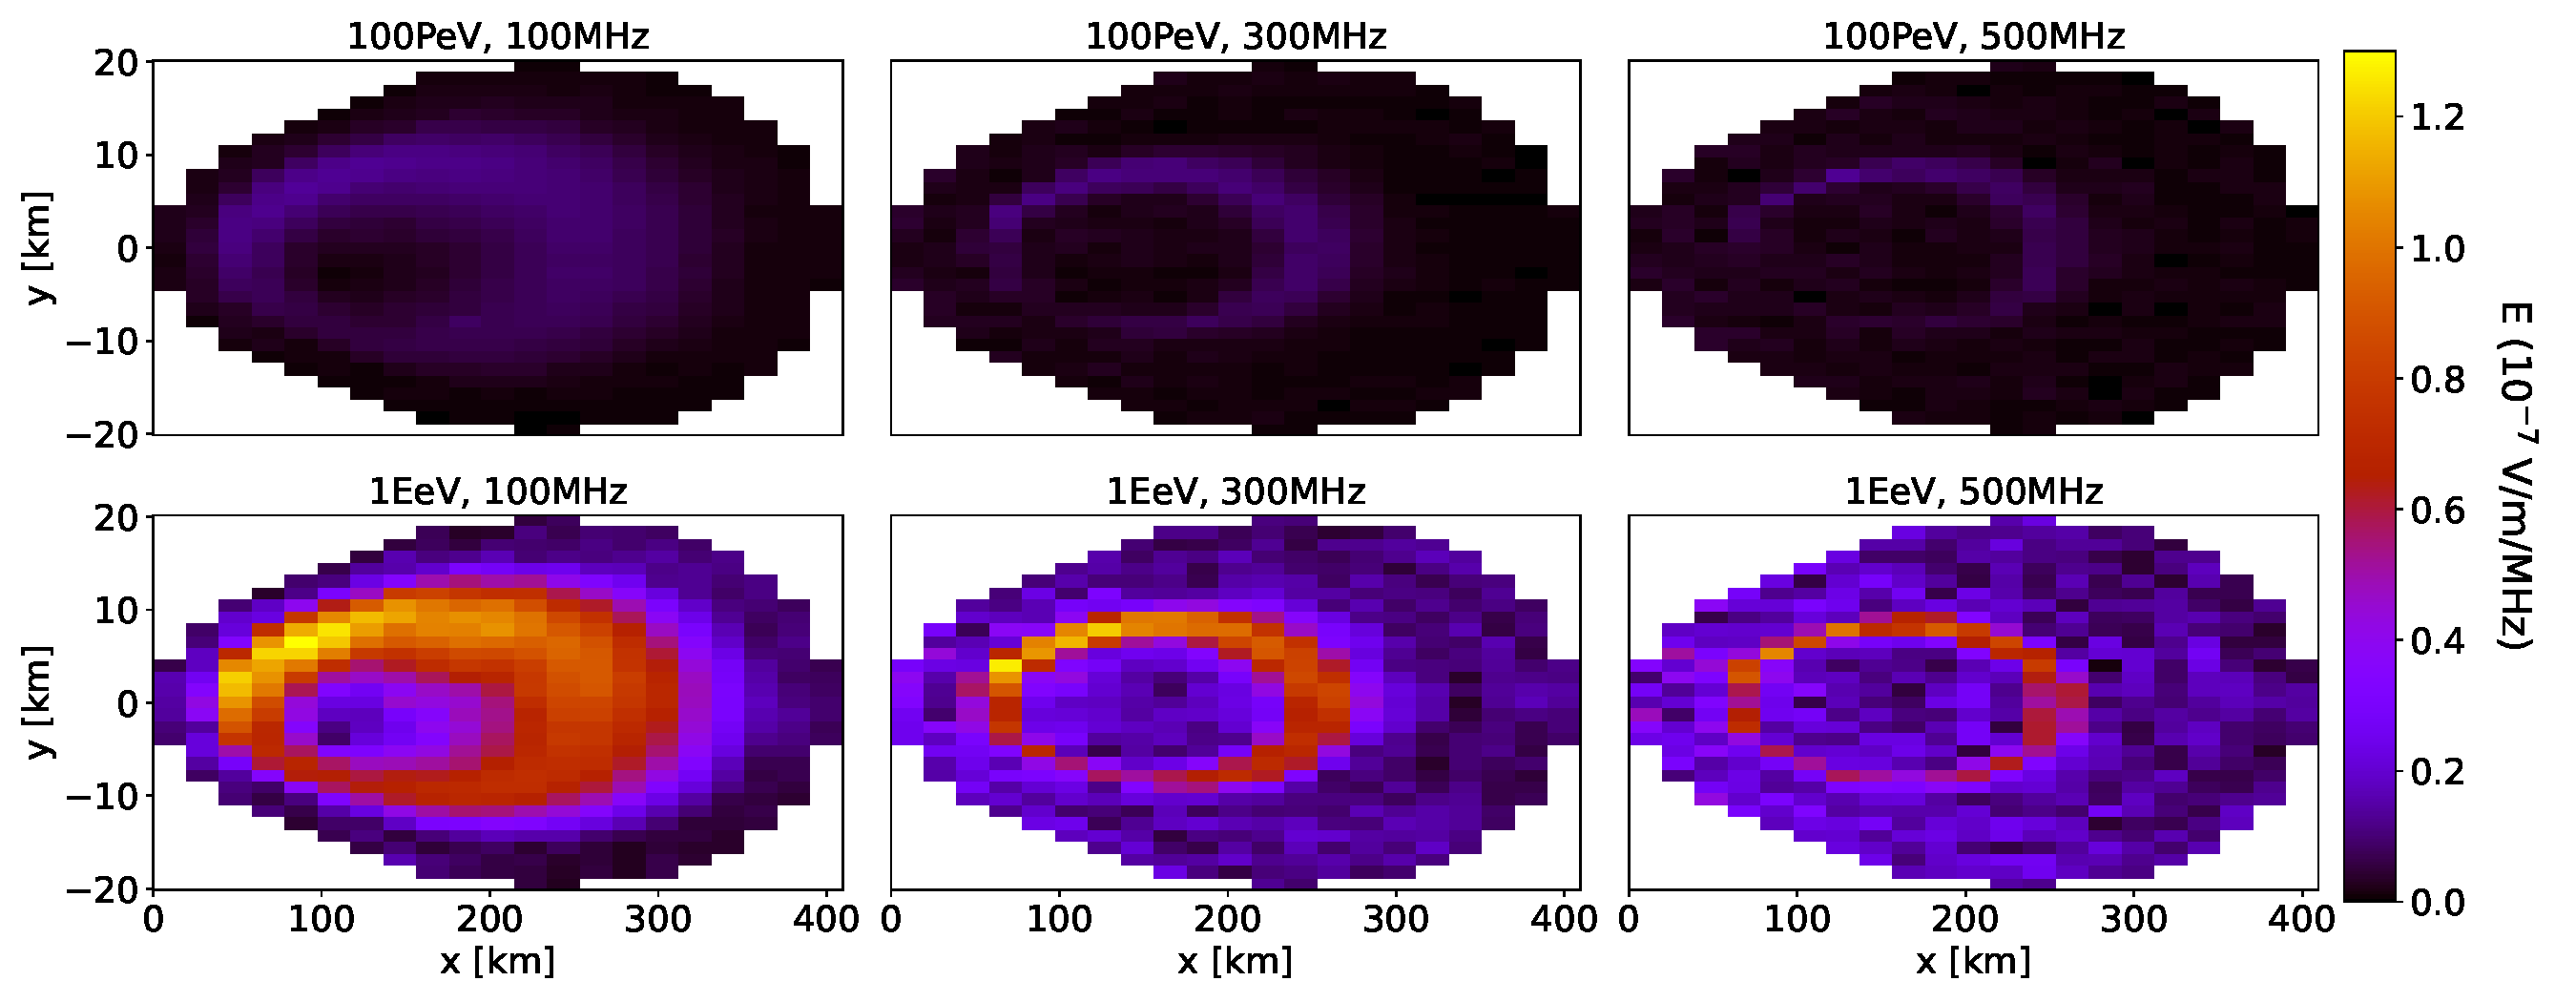
\includegraphics[width=.95\linewidth]{figures/Radio_UG/85deg_varE}
	\caption{Componentes de Fourier del campo eléctrico observado a $36\,\mathrm{km}$ de altura, para diferente energía del protón primario. Omitimos los gráficos para $E_0=10\,\mathrm{PeV}$, cuya señal es inapreciable en esta escala. El origen de coordenadas $xy$ es arbitrario.}
	\label{85deg_varE}
\end{figure}
Esta clase de enfoque podría ser viable en experimentos a altitudes no muy elevadas con detectores desplegados sobre el suelo (e.g. BEACON), aunque a mayores alturas tanto las dimensiones del cono \v{C}erenkov como la imposibilidad de contar con detectores \textit{extensos} ni perfectamente \textit{estáticos} (en globos o incluso en satélites) obliga a emplear otras técnicas, entre las que pueden encontrarse, entre otras, el estudio del tiempo de llegada de la señal al detector (i.e., el máximo de señal ocurrirá ligeramente antes en la zona del detector orientada hacia la dirección de llegada del primario).  

En cualquier caso, debemos quedarnos de lo anterior con que tanto el estudio de la forma de la elipse \v{C}erenkov registrada en detectores sobre el suelo como los retardos de la señal (entre otras técnicas) permitirían extraer información acerca de la dirección de llegada del primario. Por otra parte, el propio patrón de la radiación emitida contiene información acerca de la naturaleza de la partícula primaria. Por ejemplo, en el caso de cascadas hacia abajo en las que es posible contar con arrays de detectores sensibles a la totalidad del anillo \v{C}erenkov, las dimensiones del mismo permitirían estimar la posición del vértice del cono, i.e., del máximo del desarrollo $X_{max}$, que contiene información acerca de la masa del primario\footnote{ Por ejemplo, el máximo de cascadas iniciadas por núcleos ocurre típicamente a mayor altura en la atmósfera que para el caso de protones primarios, debido a las diferentes secciones eficaces de interacción con aire.}. Por su parte, en el caso mucho más concreto que nos ocupa, la identificación del primario sería prácticamente inmediata, ya que la observación de una cascada atmosférica iniciada \textit{por debajo} del horizonte revelaría, casi de manera inequívoca, un origen en la interacción de un neutrino tau en el interior de la Tierra.

Más allá de la estructura \textit{espacial} de la señal registrada, es evidente que la intensidad del campo eléctrico observado tiene una dependencia importante tanto con la altura del detector como con la energía de la partícula primaria. El interés de esta última cuestión es evidente al ser una de las magnitudes clave que se desea conocer de la partícula primaria; mientras que la dependencia con la altura de la posición de observación puede permitir extraer información acerca de la localización del máximo del desarrollo, de nuevo abriendo la posibilidad de identificar eventos iniciados por neutrinos tau interaccionando en el interior de la Tierra.

Para estudiar en algo más de detalle el efecto de estas dos últimas cuestiones, estudiaremos el valor máximo registrado para el campo eléctrico en las simulaciones que se han llevado a cabo. En primer lugar, podemos considerar la variación de dichos valores en función de la energía de la partícula primaria. Los valores correspondientes se presentan en la Fig. \ref{EmaxvsE}. A pesar de estar limitados por el número de simulaciones realizadas, podemos ver claramente que existe una tendencia lineal relacionando la amplitud máxima del campo eléctrico con la energía del primario. La interpretación de este comportamiento se halla en un hecho que ya mencionamos durante la caracterización del desarrollo de cascadas atmosféricas hacia arriba: el número de partículas cargadas producidas en el máximo del desarrollo es aproximadamente proporcional a la energía del primario \eqref{ec25}.
Puesto que la amplitud del campo eléctrico estará determinada fundamentalmente por la contribución de las partículas cargadas en el máximo (sobre todo $e^\pm$), el comportamiento que observamos en la Fig. \ref{EmaxvsE} debe entenderse como consecuencia directa de la dependencia lineal del número máximo de partículas con la energía:
\begin{equation}
	\left|\vect{E}\right|_{max}\propto N_{e}^{max}\propto E_0 \label{ec42}
\end{equation}
\clearpage
\begin{figure}[H]
	\centering
	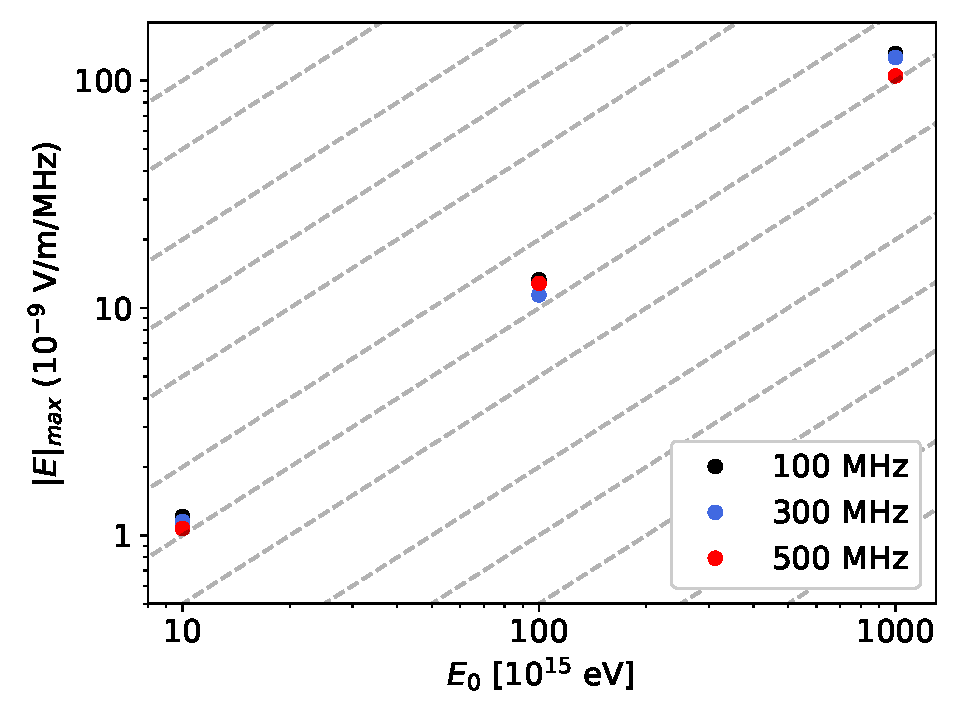
\includegraphics[width=.5\linewidth]{figures/Radio_UG/85deg_varE_36km_Emax_vs_E}
	\caption{Valor máximo de las componentes del campo eléctrico registradas a $36\,\mathrm{km}$ de altura en función de la energía del primario. Las líneas discontinuas indican el comportamiento $\left|\vect{E}\right|_{max}\propto E_0$.}
	\label{EmaxvsE}
\end{figure}
Por otra parte, para estudiar la dependencia del máximo observado con la altura del detector, hemos representado en la Fig. \ref{Emaxvsd} la variación de dichos valores con la distancia $d$  desde el nivel del suelo (que aproximadamente se corresponde con la posición del máximo del desarrollo) hasta el nivel de observación impuesto en las simulaciones, medida a lo largo del eje de la cascada (ec. \ref{ec28}). Esta elección se debe a que, para un ángulo $\theta=95^\circ$, la dependencia de la altura con la distancia a la fuente ($d$) no es lineal \eqref{ec28}.
\begin{figure}[H]
	\centering
	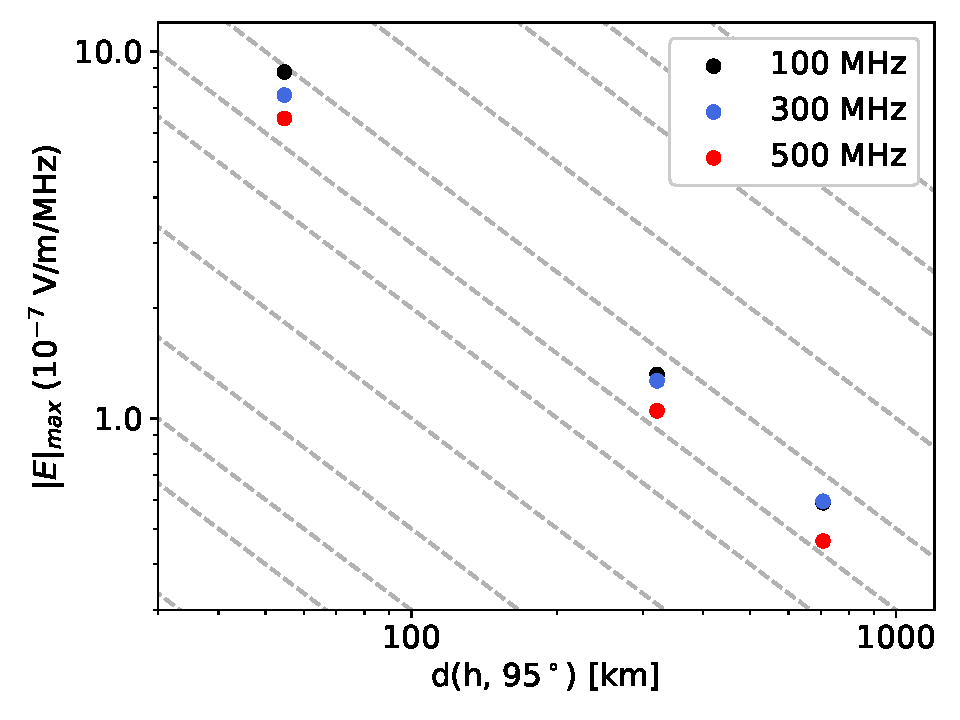
\includegraphics[width=.5\linewidth]{figures/Radio_UG/85deg_1EeV_varh_Emax_vs_d}
	\caption{Valor máximo de las componentes del campo eléctrico registradas en función de la distancia a lo largo del eje de la cascada. Las líneas discontinuas indican el comportamiento $\left|\vect{E}\right|_{max}\propto 1/d$.}
	\label{Emaxvsd}
\end{figure}

Como vemos inmediatamente, la amplitud máxima del campo eléctrico registrado decrece como la inversa de la distancia a la fuente. Naturalmente, no esperábamos un comportamiento distinto al estar observando campos de radiación.

Resumiendo, tanto el patrón de radiación emitida en cascadas atmosféricas (i.e., la forma del anillo \v{C}erenkov) como la misma intensidad del campo eléctrico y los tiempos de llegada de la señal pueden permitir extraer información acerca de la partícula primaria. Fundamentalmente, la estructura del anillo \v{C}erenkov y los retardos pueden ayudar a identificar la dirección de llegada del primario, mientras que la intensidad de la señal está relacionada con su energía y con la distancia al máximo del desarrollo, de nuevo relacionada con la dirección de llegada. Además, en los eventos que nos interesan, la determinación de la dirección de llegada implicaría con gran seguridad la identificación del origen de la cascada en un neutrino tau interaccionando en el interior de la Tierra.

Como vemos, la estructura del patrón de radiación contiene información muy valiosa acerca del primario. Sin embargo, en detectores a grandes alturas la observación de una fracción significativa de dicho patrón no es especialmente viable (con la excepción de experimentos basados en detectores sobre el terreno a gran elevación). Además, consideraciones como \eqref{ec42}, Fig. \ref{EmaxvsE} sólo son válidas si se observa el máximo de la emisión, algo que no ocurrirá en general en detectores de tamaño reducido. Esta clase de cuestiones pueden afrontarse con técnicas de análisis más detalladas, cuya explicación en detalle nos obligaría a abandonar el enfoque descriptivo de este trabajo. De manera muy breve, podemos mencionar que las simulaciones de la emisión de radiación con códigos como ZHAireS son fundamentales a la hora de extraer información de datos experimentales, ya que a partir de ellas puede realizarse una comparación entre los valores medidos y los simulados para diversas energías y naturaleza del primario. De esa manera, la información puede extraerse a partir de las condiciones iniciales que, en la simulación, reproduzcan fielmente la observación.

Por otra parte, existen observables que pueden complementar e incluso resultar más ventajosos que la amplitud del campo eléctrico a la hora de trabajar con datos reales. Por ejemplo, la polarización puede aportar información \textit{extra} acerca de la posición del máximo (e.g. mediante estudios detallados de las contribuciones geomagnética y Askaryan), mientras que el estudio del flujo integrado de energía recibida\footnote{ Integral temporal de la intensidad de la señal, $\int\left|E\right|^2dt$} permite trabajar con un observable más estable frente a fluctuaciones y facilita la distinción entre señal y ruido ambiente.

De lo anterior, debemos quedarnos con que mediante el estudio de observables \textit{sencillos} hemos sido capaces de describir la radiación electromagnética emitida en cascadas atmosféricas hacia arriba, y hemos visto que dicha emisión contiene gran cantidad de información acerca de la naturaleza de la partícula primaria, gracias a la que podrían llegar a identificarse (con las técnicas adecuadas) eventos iniciados por neutrinos de altas energías y origen astrofísico.
	\clearpage %cleardoublepage pode meter paxinas en branco. Non e obrigatorio. Tampouco para a 
	\section{Conclusiones}
	La observación de neutrinos de muy altas energías y origen astrofísico se ha convertido en uno de los objetivos científicos fundamentales dentro del marco de la astronomía de multi-mensajeros y la Física de Astropartículas, debido a la gran ocasión que su detección y la medición de sus propiedades (dirección de llegada, espectro de energías, ...) nos ofrece para aumentar nuestro conocimiento sobre los fenómenos más energéticos del Universo.
	
	Dentro de las numerosas propuestas experimentales encaminadas al estudio de neutrinos de muy altas energías, las técnicas de radiodetección han experimentado un crecimiento significativo en los últimos años, debido tanto a su potencial para obtener información acerca de la partícula primaria como por la relativa facilidad para desplegar detectores cubriendo grandes áreas y/o alcanzando altas exposiciones. Además, la posibilidad de disponer de antenas desplegadas a grandes alturas permite ser sensibles a las interacciones de neutrinos tau en el interior de la Tierra, aumentando enormemente las posibilidades de observación.
	
	En este trabajo, hemos estudiado tanto el desarrollo de las cascadas de partículas atmosféricas que aparecerían en eventos iniciados por neutrinos tau de origen astrofísico como la radiación electromagnética asociada que se observaría a diversas alturas, entre las que hemos incluido las previstas para experimentos futuros como BEACON y PUEO. Gracias a la caracterización de las cascadas atmosféricas hacia arriba de gran inclinación, que además hemos interpretado en términos \textit{microscópicos}, hemos podido comprobar el efecto que magnitudes como la energía del primario y su dirección tienen en el desarrollo de la cascada. Por otra parte, gracias a simulaciones partiendo de principios básicos, hemos conseguido estudiar la radiación electromagnética asociada a estos eventos, cuya dependencia con los parámetros y evolución de la cascada permiten relacionar el campo eléctrico observado con las propiedades clave de la partícula primaria. A partir de consideraciones sencillas, hemos comprobado la posibilidad de extraer dicha información a través del estudio de la emisión en radiofrecuencias.
	
	En los próximos años, la realización de experimentos basados en este principio de detección y el estudio de la información recogida con las técnicas de análisis adecuadas, que podrá ser complementada con los datos recogidos por experimentos sensibles a otros aspectos del desarrollo de cascadas, abrirá por tanto la posibilidad de aumentar en gran medida nuestro conocimiento sobre el Universo a las energías más altas exploradas hasta la fecha, desde la escala de los fenómenos astrofísicos más violentos conocidos hasta la de las mismas interacciones fundamentales y su estructura a energías cada vez mayores.
	%%%%%%%Bibliografía
	\clearpage
	\fancyhead{}
	\appendix
	\phantomsection
	\markboth{REFERENCIAS}{REFERENCIAS}  
	\addcontentsline{toc}{section}{Referencias} 
	\nocite{*}
	\bibliography{TFMbib}
	\bibliographystyle{apalike}

	
\end{document}